\PassOptionsToPackage{unicode=true}{hyperref} % options for packages loaded elsewhere
\PassOptionsToPackage{hyphens}{url}
%
\documentclass[]{article}
\usepackage{lmodern}
\usepackage{amssymb,amsmath}
\usepackage{ifxetex,ifluatex}
\usepackage{fixltx2e} % provides \textsubscript
\ifnum 0\ifxetex 1\fi\ifluatex 1\fi=0 % if pdftex
  \usepackage[T1]{fontenc}
  \usepackage[utf8]{inputenc}
  \usepackage{textcomp} % provides euro and other symbols
\else % if luatex or xelatex
  \usepackage{unicode-math}
  \defaultfontfeatures{Ligatures=TeX,Scale=MatchLowercase}
\fi
% use upquote if available, for straight quotes in verbatim environments
\IfFileExists{upquote.sty}{\usepackage{upquote}}{}
% use microtype if available
\IfFileExists{microtype.sty}{%
\usepackage[]{microtype}
\UseMicrotypeSet[protrusion]{basicmath} % disable protrusion for tt fonts
}{}
\IfFileExists{parskip.sty}{%
\usepackage{parskip}
}{% else
\setlength{\parindent}{0pt}
\setlength{\parskip}{6pt plus 2pt minus 1pt}
}
\usepackage{hyperref}
\hypersetup{
            pdftitle={Using citizen science to parse climatic and landcover influences on bird occupancy within a tropical biodiversity hotspot},
            pdfauthor={Vijay Ramesh; Pratik R. Gupte; Morgan W. Tingley; VV Robin; Ruth DeFries},
            pdfborder={0 0 0},
            breaklinks=true}
\urlstyle{same}  % don't use monospace font for urls
\usepackage[margin=1in]{geometry}
\usepackage{color}
\usepackage{fancyvrb}
\newcommand{\VerbBar}{|}
\newcommand{\VERB}{\Verb[commandchars=\\\{\}]}
\DefineVerbatimEnvironment{Highlighting}{Verbatim}{commandchars=\\\{\}}
% Add ',fontsize=\small' for more characters per line
\newenvironment{Shaded}{}{}
\newcommand{\AlertTok}[1]{\textcolor[rgb]{1.00,0.00,0.00}{#1}}
\newcommand{\AnnotationTok}[1]{\textcolor[rgb]{0.00,0.50,0.00}{#1}}
\newcommand{\AttributeTok}[1]{#1}
\newcommand{\BaseNTok}[1]{#1}
\newcommand{\BuiltInTok}[1]{#1}
\newcommand{\CharTok}[1]{\textcolor[rgb]{0.00,0.50,0.50}{#1}}
\newcommand{\CommentTok}[1]{\textcolor[rgb]{0.00,0.50,0.00}{#1}}
\newcommand{\CommentVarTok}[1]{\textcolor[rgb]{0.00,0.50,0.00}{#1}}
\newcommand{\ConstantTok}[1]{#1}
\newcommand{\ControlFlowTok}[1]{\textcolor[rgb]{0.00,0.00,1.00}{#1}}
\newcommand{\DataTypeTok}[1]{#1}
\newcommand{\DecValTok}[1]{#1}
\newcommand{\DocumentationTok}[1]{\textcolor[rgb]{0.00,0.50,0.00}{#1}}
\newcommand{\ErrorTok}[1]{\textcolor[rgb]{1.00,0.00,0.00}{\textbf{#1}}}
\newcommand{\ExtensionTok}[1]{#1}
\newcommand{\FloatTok}[1]{#1}
\newcommand{\FunctionTok}[1]{#1}
\newcommand{\ImportTok}[1]{#1}
\newcommand{\InformationTok}[1]{\textcolor[rgb]{0.00,0.50,0.00}{#1}}
\newcommand{\KeywordTok}[1]{\textcolor[rgb]{0.00,0.00,1.00}{#1}}
\newcommand{\NormalTok}[1]{#1}
\newcommand{\OperatorTok}[1]{#1}
\newcommand{\OtherTok}[1]{\textcolor[rgb]{1.00,0.25,0.00}{#1}}
\newcommand{\PreprocessorTok}[1]{\textcolor[rgb]{1.00,0.25,0.00}{#1}}
\newcommand{\RegionMarkerTok}[1]{#1}
\newcommand{\SpecialCharTok}[1]{\textcolor[rgb]{0.00,0.50,0.50}{#1}}
\newcommand{\SpecialStringTok}[1]{\textcolor[rgb]{0.00,0.50,0.50}{#1}}
\newcommand{\StringTok}[1]{\textcolor[rgb]{0.00,0.50,0.50}{#1}}
\newcommand{\VariableTok}[1]{#1}
\newcommand{\VerbatimStringTok}[1]{\textcolor[rgb]{0.00,0.50,0.50}{#1}}
\newcommand{\WarningTok}[1]{\textcolor[rgb]{0.00,0.50,0.00}{\textbf{#1}}}
\usepackage{longtable,booktabs}
% Fix footnotes in tables (requires footnote package)
\IfFileExists{footnote.sty}{\usepackage{footnote}\makesavenoteenv{longtable}}{}
\usepackage{graphicx,grffile}
\makeatletter
\def\maxwidth{\ifdim\Gin@nat@width>\linewidth\linewidth\else\Gin@nat@width\fi}
\def\maxheight{\ifdim\Gin@nat@height>\textheight\textheight\else\Gin@nat@height\fi}
\makeatother
% Scale images if necessary, so that they will not overflow the page
% margins by default, and it is still possible to overwrite the defaults
% using explicit options in \includegraphics[width, height, ...]{}
\setkeys{Gin}{width=\maxwidth,height=\maxheight,keepaspectratio}
\setlength{\emergencystretch}{3em}  % prevent overfull lines
\providecommand{\tightlist}{%
  \setlength{\itemsep}{0pt}\setlength{\parskip}{0pt}}
\setcounter{secnumdepth}{5}
% Redefines (sub)paragraphs to behave more like sections
\ifx\paragraph\undefined\else
\let\oldparagraph\paragraph
\renewcommand{\paragraph}[1]{\oldparagraph{#1}\mbox{}}
\fi
\ifx\subparagraph\undefined\else
\let\oldsubparagraph\subparagraph
\renewcommand{\subparagraph}[1]{\oldsubparagraph{#1}\mbox{}}
\fi

% set default figure placement to htbp
\makeatletter
\def\fps@figure{htbp}
\makeatother


\title{Using citizen science to parse climatic and landcover influences on bird occupancy within a tropical biodiversity hotspot}
\author{Vijay Ramesh \and Pratik R. Gupte \and Morgan W. Tingley \and VV Robin \and Ruth DeFries}
\date{2020-12-18}

\begin{document}
\maketitle

{
\setcounter{tocdepth}{2}
\tableofcontents
}
\hypertarget{introduction}{%
\section{Introduction}\label{introduction}}

This is the readable version containing analysis that models associations between environmental predictors (climate and landcover) and citizen science observations of birds across the Nilgiri and Anamalai Hills of the Western Ghats Biodiversity Hotspot.

Methods and format are derived from \href{https://cornelllabofornithology.github.io/ebird-best-practices/}{Strimas-Mackey et al.}.

\hypertarget{attribution}{%
\subsection{Attribution}\label{attribution}}

Please contact the following in case of interest in the project.

\begin{itemize}
\tightlist
\item
  Vijay Ramesh (lead author)

  \begin{itemize}
  \tightlist
  \item
    PhD student, Columbia University
  \end{itemize}
\item
  Pratik Gupte (repo maintainer)

  \begin{itemize}
  \tightlist
  \item
    PhD student, University of Groningen
  \end{itemize}
\end{itemize}

\hypertarget{data-access}{%
\subsection{Data access}\label{data-access}}

The data used in this work are available from \href{http://ebird.org/data/download}{eBird}.

\hypertarget{data-processing}{%
\subsection{Data processing}\label{data-processing}}

The data processing for this project is described in the following sections. Navigate through them using the links in the sidebar.

\hypertarget{main-text-figure-1}{%
\subsection{Main Text Figure 1}\label{main-text-figure-1}}

\begin{figure}
\centering
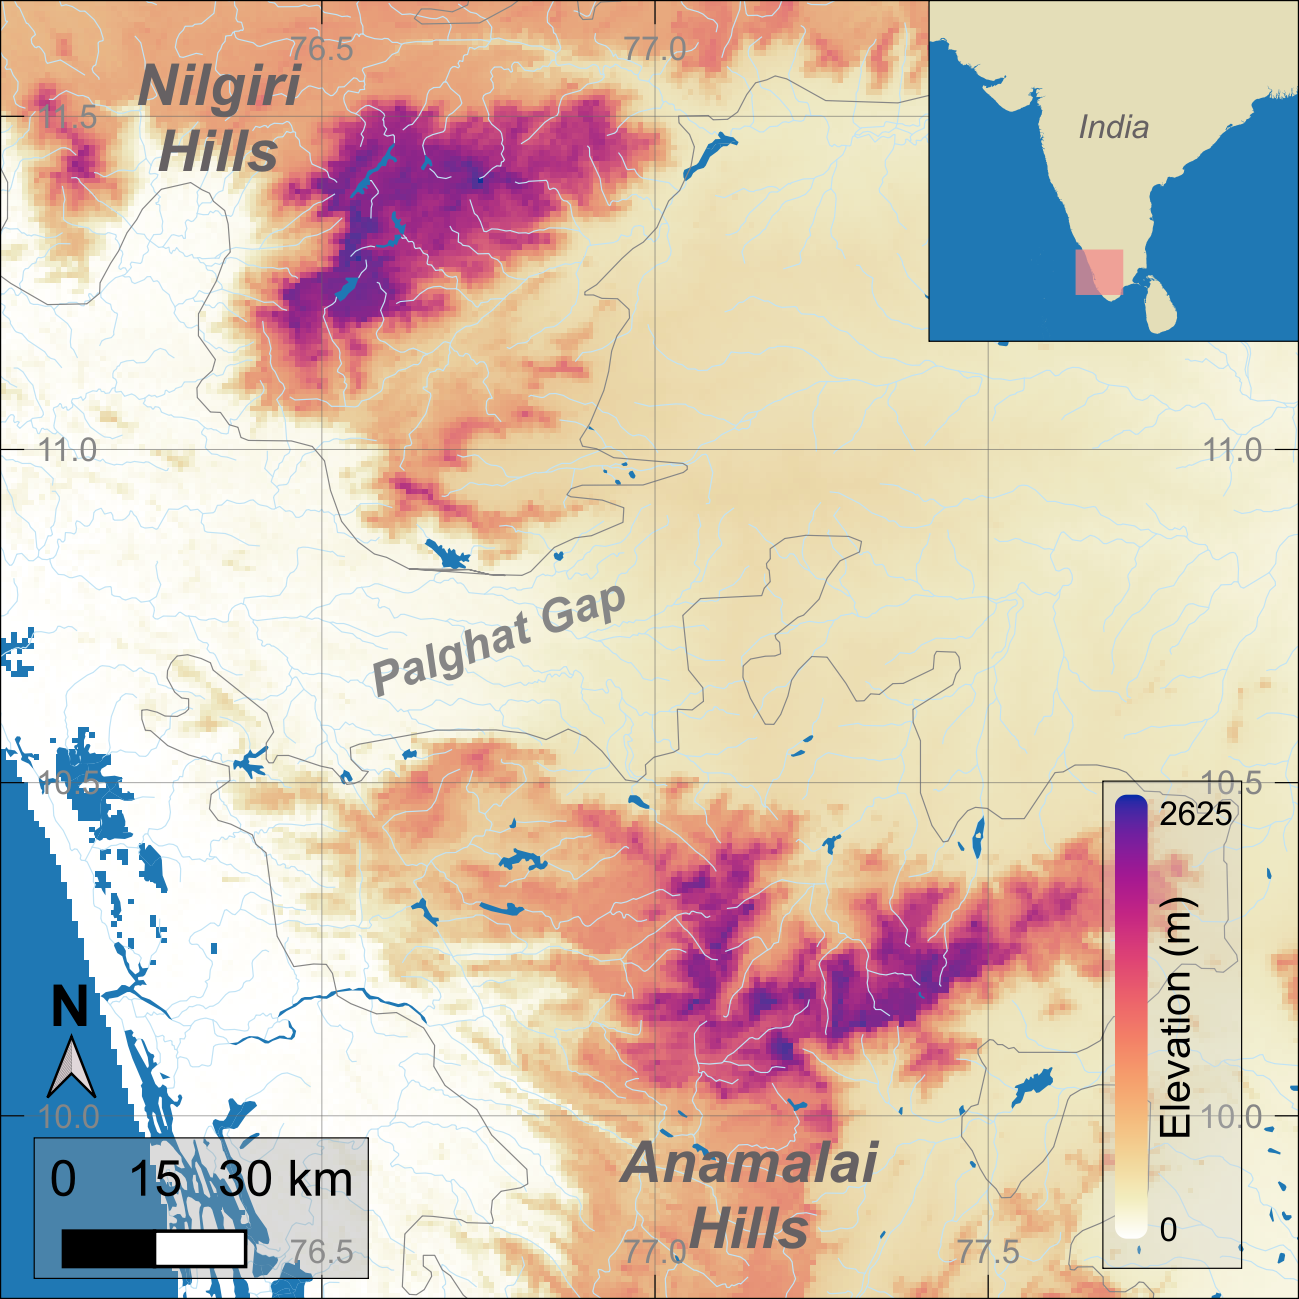
\includegraphics{figs/fig_01_elevation.png}
\caption{A shaded relief of the study area - the Nilgiri and the Anamalai hills are shown in this figure. This map was made using the SRTM digital elevation model at a spatial resolution of 1km and data from Natural Earth were used to outline boundaries of water bodies.}
\end{figure}

\hypertarget{preparing-ebird-data}{%
\section{Preparing eBird Data}\label{preparing-ebird-data}}

\hypertarget{prepare-libraries-and-data-sources}{%
\subsection{Prepare libraries and data sources}\label{prepare-libraries-and-data-sources}}

\begin{Shaded}
\begin{Highlighting}[]

\CommentTok{# load libs}
\KeywordTok{library}\NormalTok{(tidyverse)}
\KeywordTok{library}\NormalTok{(readr)}
\KeywordTok{library}\NormalTok{(sf)}
\KeywordTok{library}\NormalTok{(auk)}
\KeywordTok{library}\NormalTok{(readxl)}

\CommentTok{# custom sum function}
\NormalTok{sum.no.na <-}\StringTok{ }\ControlFlowTok{function}\NormalTok{(x) \{}
  \KeywordTok{sum}\NormalTok{(x, }\DataTypeTok{na.rm =}\NormalTok{ T)}
\NormalTok{\}}

\CommentTok{# set file paths for auk functions}
\NormalTok{f_in_ebd <-}\StringTok{ }\KeywordTok{file.path}\NormalTok{(}\StringTok{"data/ebd_IN_relApr-2020.txt"}\NormalTok{)}
\NormalTok{f_in_sampling <-}\StringTok{ }\KeywordTok{file.path}\NormalTok{(}\StringTok{"data/ebd_sampling_relApr-2020.txt"}\NormalTok{)}
\end{Highlighting}
\end{Shaded}

\hypertarget{filter-data}{%
\subsection{Filter data}\label{filter-data}}

\begin{Shaded}
\begin{Highlighting}[]
\CommentTok{# add species of interest}
\NormalTok{specieslist <-}\StringTok{ }\KeywordTok{read.csv}\NormalTok{(}\StringTok{"data/species_list.csv"}\NormalTok{)}
\NormalTok{speciesOfInterest <-}\StringTok{ }\KeywordTok{as.character}\NormalTok{(specieslist}\OperatorTok{$}\NormalTok{scientific_name)}
\end{Highlighting}
\end{Shaded}

\begin{Shaded}
\begin{Highlighting}[]

\CommentTok{# run filters using auk packages}
\NormalTok{ebd_filters <-}\StringTok{ }\KeywordTok{auk_ebd}\NormalTok{(f_in_ebd, f_in_sampling) }\OperatorTok
\StringTok{  }\KeywordTok{auk_species}\NormalTok{(speciesOfInterest) }\OperatorTok
\StringTok{  }\KeywordTok{auk_country}\NormalTok{(}\DataTypeTok{country =} \StringTok{"IN"}\NormalTok{) }\OperatorTok
\StringTok{  }\KeywordTok{auk_state}\NormalTok{(}\KeywordTok{c}\NormalTok{(}\StringTok{"IN-KL"}\NormalTok{, }\StringTok{"IN-TN"}\NormalTok{, }\StringTok{"IN-KA"}\NormalTok{)) }\OperatorTok\StringTok{ }\CommentTok{# Restricting geography to TamilNadu, Kerala & Karnataka}
\StringTok{  }\KeywordTok{auk_date}\NormalTok{(}\KeywordTok{c}\NormalTok{(}\StringTok{"2013-01-01"}\NormalTok{, }\StringTok{"2019-12-31"}\NormalTok{)) }\OperatorTok
\StringTok{  }\KeywordTok{auk_complete}\NormalTok{()}

\CommentTok{# check filters}
\NormalTok{ebd_filters}
\end{Highlighting}
\end{Shaded}

Below code need not be run if it has been filtered once already and the above path leads to the right dataset. NB: This is a computation heavy process, run with caution.

\begin{Shaded}
\begin{Highlighting}[]

\CommentTok{# specify output location and perform filter}
\NormalTok{f_out_ebd <-}\StringTok{ "data/eBirdDataWG_filtered.txt"}
\NormalTok{f_out_sampling <-}\StringTok{ "data/eBirdSamplingDataWG_filtered.txt"}
\end{Highlighting}
\end{Shaded}

\begin{Shaded}
\begin{Highlighting}[]
\NormalTok{ebd_filtered <-}\StringTok{ }\KeywordTok{auk_filter}\NormalTok{(ebd_filters,}
  \DataTypeTok{file =}\NormalTok{ f_out_ebd,}
  \DataTypeTok{file_sampling =}\NormalTok{ f_out_sampling, }\DataTypeTok{overwrite =} \OtherTok{TRUE}
\NormalTok{)}
\end{Highlighting}
\end{Shaded}

\hypertarget{process-filtered-data}{%
\subsection{Process filtered data}\label{process-filtered-data}}

\begin{Shaded}
\begin{Highlighting}[]
\CommentTok{# read in the data}
\NormalTok{ebd <-}\StringTok{ }\KeywordTok{read_ebd}\NormalTok{(f_out_ebd)}
\end{Highlighting}
\end{Shaded}

\begin{Shaded}
\begin{Highlighting}[]
\CommentTok{# fill zeroes}
\NormalTok{zf <-}\StringTok{ }\KeywordTok{auk_zerofill}\NormalTok{(f_out_ebd, f_out_sampling)}
\NormalTok{new_zf <-}\StringTok{ }\KeywordTok{collapse_zerofill}\NormalTok{(zf) }\CommentTok{# Creates a new zero-filled dataframe with a 0 marked for each checklist when the bird was not observed}
\end{Highlighting}
\end{Shaded}

\begin{Shaded}
\begin{Highlighting}[]
\CommentTok{# choose columns of interest}
\NormalTok{columnsOfInterest <-}\StringTok{ }\KeywordTok{c}\NormalTok{(}
  \StringTok{"checklist_id"}\NormalTok{, }\StringTok{"scientific_name"}\NormalTok{, }\StringTok{"common_name"}\NormalTok{,}
  \StringTok{"observation_count"}\NormalTok{, }\StringTok{"locality"}\NormalTok{, }\StringTok{"locality_id"}\NormalTok{,}
  \StringTok{"locality_type"}\NormalTok{, }\StringTok{"latitude"}\NormalTok{, }\StringTok{"longitude"}\NormalTok{,}
  \StringTok{"observation_date"}\NormalTok{, }\StringTok{"time_observations_started"}\NormalTok{,}
  \StringTok{"observer_id"}\NormalTok{, }\StringTok{"sampling_event_identifier"}\NormalTok{,}
  \StringTok{"protocol_type"}\NormalTok{, }\StringTok{"duration_minutes"}\NormalTok{,}
  \StringTok{"effort_distance_km"}\NormalTok{, }\StringTok{"effort_area_ha"}\NormalTok{,}
  \StringTok{"number_observers"}\NormalTok{, }\StringTok{"species_observed"}\NormalTok{,}
  \StringTok{"reviewed"}
\NormalTok{)}

\CommentTok{# make list of presence and absence data and choose cols of interest}
\NormalTok{data <-}\StringTok{ }\KeywordTok{list}\NormalTok{(ebd, new_zf) }\OperatorTok
\StringTok{  }\KeywordTok{map}\NormalTok{(}\ControlFlowTok{function}\NormalTok{(x) \{}
\NormalTok{    x }\OperatorTok\StringTok{ }\KeywordTok{select}\NormalTok{(}\KeywordTok{one_of}\NormalTok{(columnsOfInterest))}
\NormalTok{  \})}

\CommentTok{# remove zerofills to save working memory}
\KeywordTok{rm}\NormalTok{(zf, new_zf)}
\KeywordTok{gc}\NormalTok{()}

\CommentTok{# check presence and absence in absences df, remove essentially the presences df}
\NormalTok{data[[}\DecValTok{2}\NormalTok{]] <-}\StringTok{ }\NormalTok{data[[}\DecValTok{2}\NormalTok{]] }\OperatorTok\StringTok{ }\KeywordTok{filter}\NormalTok{(species_observed }\OperatorTok{==}\StringTok{ }\NormalTok{F)}
\end{Highlighting}
\end{Shaded}

\hypertarget{spatial-filter}{%
\subsection{Spatial filter}\label{spatial-filter}}

\begin{Shaded}
\begin{Highlighting}[]

\CommentTok{# load shapefiles of hill ranges}
\KeywordTok{library}\NormalTok{(sf)}
\NormalTok{hills <-}\StringTok{ }\KeywordTok{st_read}\NormalTok{(}\StringTok{"data/spatial/hillsShapefile/Nil_Ana_Pal.shp"}\NormalTok{)}

\CommentTok{# write a prelim filter by bounding box}
\NormalTok{box <-}\StringTok{ }\KeywordTok{st_bbox}\NormalTok{(hills)}

\CommentTok{# get data spatial coordinates}
\NormalTok{dataLocs <-}\StringTok{ }\NormalTok{data }\OperatorTok
\StringTok{  }\KeywordTok{map}\NormalTok{(}\ControlFlowTok{function}\NormalTok{(x) \{}
    \KeywordTok{select}\NormalTok{(x, longitude, latitude) }\OperatorTok
\StringTok{      }\KeywordTok{filter}\NormalTok{(}\KeywordTok{between}\NormalTok{(longitude, box[}\StringTok{"xmin"}\NormalTok{], box[}\StringTok{"xmax"}\NormalTok{]) }\OperatorTok{&}
\StringTok{        }\KeywordTok{between}\NormalTok{(latitude, box[}\StringTok{"ymin"}\NormalTok{], box[}\StringTok{"ymax"}\NormalTok{]))}
\NormalTok{  \}) }\OperatorTok
\StringTok{  }\KeywordTok{bind_rows}\NormalTok{() }\OperatorTok
\StringTok{  }\KeywordTok{distinct}\NormalTok{() }\OperatorTok
\StringTok{  }\KeywordTok{st_as_sf}\NormalTok{(}\DataTypeTok{coords =} \KeywordTok{c}\NormalTok{(}\StringTok{"longitude"}\NormalTok{, }\StringTok{"latitude"}\NormalTok{)) }\OperatorTok
\StringTok{  }\KeywordTok{st_set_crs}\NormalTok{(}\DecValTok{4326}\NormalTok{) }\OperatorTok
\StringTok{  }\KeywordTok{st_intersection}\NormalTok{(hills)}

\CommentTok{# get simplified data and drop geometry}
\NormalTok{dataLocs <-}\StringTok{ }\KeywordTok{mutate}\NormalTok{(dataLocs, }\DataTypeTok{spatialKeep =}\NormalTok{ T) }\OperatorTok
\StringTok{  }\KeywordTok{bind_cols}\NormalTok{(., }\KeywordTok{as_tibble}\NormalTok{(}\KeywordTok{st_coordinates}\NormalTok{(dataLocs))) }\OperatorTok
\StringTok{  }\KeywordTok{st_drop_geometry}\NormalTok{()}

\CommentTok{# bind to data and then filter}
\NormalTok{data <-}\StringTok{ }\NormalTok{data }\OperatorTok
\StringTok{  }\KeywordTok{map}\NormalTok{(}\ControlFlowTok{function}\NormalTok{(x) \{}
    \KeywordTok{left_join}\NormalTok{(x, dataLocs, }\DataTypeTok{by =} \KeywordTok{c}\NormalTok{(}\StringTok{"longitude"}\NormalTok{ =}\StringTok{ "X"}\NormalTok{, }\StringTok{"latitude"}\NormalTok{ =}\StringTok{ "Y"}\NormalTok{)) }\OperatorTok
\StringTok{      }\KeywordTok{filter}\NormalTok{(spatialKeep }\OperatorTok{==}\StringTok{ }\NormalTok{T) }\OperatorTok
\StringTok{      }\KeywordTok{select}\NormalTok{(}\OperatorTok{-}\NormalTok{Id, }\OperatorTok{-}\NormalTok{spatialKeep)}
\NormalTok{  \})}
\end{Highlighting}
\end{Shaded}

\begin{Shaded}
\begin{Highlighting}[]
\CommentTok{# save a temp data file}
\KeywordTok{save}\NormalTok{(data, }\DataTypeTok{file =} \StringTok{"data/data_temp.rdata"}\NormalTok{)}
\end{Highlighting}
\end{Shaded}

\hypertarget{handle-presence-data}{%
\subsection{Handle presence data}\label{handle-presence-data}}

\begin{Shaded}
\begin{Highlighting}[]

\CommentTok{# in the first set, replace X, for presences, with 1}
\NormalTok{data[[}\DecValTok{1}\NormalTok{]] <-}\StringTok{ }\NormalTok{data[[}\DecValTok{1}\NormalTok{]] }\OperatorTok
\StringTok{  }\KeywordTok{mutate}\NormalTok{(}\DataTypeTok{observation_count =} \KeywordTok{ifelse}\NormalTok{(observation_count }\OperatorTok{==}\StringTok{ "X"}\NormalTok{,}
    \StringTok{"1"}\NormalTok{, observation_count}
\NormalTok{  ))}

\CommentTok{# remove records where duration is 0}
\NormalTok{data <-}\StringTok{ }\KeywordTok{map}\NormalTok{(data, }\ControlFlowTok{function}\NormalTok{(x) }\KeywordTok{filter}\NormalTok{(x, duration_minutes }\OperatorTok{>}\StringTok{ }\DecValTok{0}\NormalTok{))}

\CommentTok{# group data by site and sampling event identifier}
\CommentTok{# then, summarise relevant variables as the sum}
\NormalTok{dataGrouped <-}\StringTok{ }\KeywordTok{map}\NormalTok{(data, }\ControlFlowTok{function}\NormalTok{(x) \{}
\NormalTok{  x }\OperatorTok
\StringTok{    }\KeywordTok{group_by}\NormalTok{(sampling_event_identifier) }\OperatorTok
\StringTok{    }\KeywordTok{summarise_at}\NormalTok{(}
      \KeywordTok{vars}\NormalTok{(}
\NormalTok{        duration_minutes, effort_distance_km,}
\NormalTok{        effort_area_ha}
\NormalTok{      ),}
      \KeywordTok{list}\NormalTok{(sum.no.na)}
\NormalTok{    )}
\NormalTok{\})}

\CommentTok{# bind rows combining data frames, and filter}
\NormalTok{dataGrouped <-}\StringTok{ }\KeywordTok{bind_rows}\NormalTok{(dataGrouped) }\OperatorTok
\StringTok{  }\KeywordTok{filter}\NormalTok{(}
\NormalTok{    duration_minutes }\OperatorTok{<=}\StringTok{ }\DecValTok{300}\NormalTok{,}
\NormalTok{    effort_distance_km }\OperatorTok{<=}\StringTok{ }\DecValTok{5}\NormalTok{,}
\NormalTok{    effort_area_ha }\OperatorTok{<=}\StringTok{ }\DecValTok{500}
\NormalTok{  )}

\CommentTok{# get data identifiers, such as sampling identifier etc}
\NormalTok{dataConstants <-}\StringTok{ }\NormalTok{data }\OperatorTok
\StringTok{  }\KeywordTok{bind_rows}\NormalTok{() }\OperatorTok
\StringTok{  }\KeywordTok{select}\NormalTok{(}
\NormalTok{    sampling_event_identifier, time_observations_started,}
\NormalTok{    locality, locality_type, locality_id,}
\NormalTok{    observer_id, observation_date, scientific_name,}
\NormalTok{    observation_count, protocol_type, number_observers,}
\NormalTok{    longitude, latitude}
\NormalTok{  )}

\CommentTok{# join the summarised data with the identifiers,}
\CommentTok{# using sampling_event_identifier as the key}
\NormalTok{dataGrouped <-}\StringTok{ }\KeywordTok{left_join}\NormalTok{(dataGrouped, dataConstants,}
  \DataTypeTok{by =} \StringTok{"sampling_event_identifier"}
\NormalTok{)}

\CommentTok{# remove checklists or seis with more than 10 obervers}
\KeywordTok{count}\NormalTok{(dataGrouped, number_observers }\OperatorTok{>}\StringTok{ }\DecValTok{10}\NormalTok{) }\CommentTok{# count how many have 10+ obs}
\NormalTok{dataGrouped <-}\StringTok{ }\KeywordTok{filter}\NormalTok{(dataGrouped, number_observers }\OperatorTok{<=}\StringTok{ }\DecValTok{10}\NormalTok{)}
\end{Highlighting}
\end{Shaded}

\hypertarget{add-decimal-time}{%
\subsection{Add decimal time}\label{add-decimal-time}}

\begin{Shaded}
\begin{Highlighting}[]

\CommentTok{# assign present or not, and get time in decimal hours since midnight}
\KeywordTok{library}\NormalTok{(lubridate)}
\NormalTok{time_to_decimal <-}\StringTok{ }\ControlFlowTok{function}\NormalTok{(x) \{}
\NormalTok{  x <-}\StringTok{ }\KeywordTok{hms}\NormalTok{(x, }\DataTypeTok{quiet =} \OtherTok{TRUE}\NormalTok{)}
  \KeywordTok{hour}\NormalTok{(x) }\OperatorTok{+}\StringTok{ }\KeywordTok{minute}\NormalTok{(x) }\OperatorTok{/}\StringTok{ }\DecValTok{60} \OperatorTok{+}\StringTok{ }\KeywordTok{second}\NormalTok{(x) }\OperatorTok{/}\StringTok{ }\DecValTok{3600}
\NormalTok{\}}

\CommentTok{# will cause issues if using time obs started as a linear effect and not quadratic}
\NormalTok{dataGrouped <-}\StringTok{ }\KeywordTok{mutate}\NormalTok{(dataGrouped,}
  \DataTypeTok{pres_abs =}\NormalTok{ observation_count }\OperatorTok{>=}\StringTok{ }\DecValTok{1}\NormalTok{,}
  \DataTypeTok{decimalTime =} \KeywordTok{time_to_decimal}\NormalTok{(time_observations_started)}
\NormalTok{)}

\CommentTok{# check class of dataGrouped, make sure not sf}
\NormalTok{assertthat}\OperatorTok{::}\KeywordTok{assert_that}\NormalTok{(}\OperatorTok{!}\StringTok{"sf"} \OperatorTok\StringTok{ }\KeywordTok{class}\NormalTok{(dataGrouped))}
\end{Highlighting}
\end{Shaded}

This data is saved to file.

\begin{Shaded}
\begin{Highlighting}[]

\CommentTok{# save a temp data file}
\KeywordTok{save}\NormalTok{(dataGrouped, }\DataTypeTok{file =} \StringTok{"data/data_prelim_processing.rdata"}\NormalTok{)}
\end{Highlighting}
\end{Shaded}

\hypertarget{preparing-landscape-data}{%
\section{Preparing Landscape Data}\label{preparing-landscape-data}}

Here, we prepare environmental layers which we have accessed as raster images from remote sensing platforms using Google Earth Engine.
The GEE code can be found in a separate file.
The goal here is to resample all rasters so that they have the same resolution of 1km cells.

\hypertarget{prepare-libraries}{%
\subsection{Prepare libraries}\label{prepare-libraries}}

We load some common libraries for raster processing and define a custom mode function.

\begin{Shaded}
\begin{Highlighting}[]

\CommentTok{# load libs}
\KeywordTok{library}\NormalTok{(raster)}
\KeywordTok{library}\NormalTok{(stringi)}
\KeywordTok{library}\NormalTok{(glue)}
\KeywordTok{library}\NormalTok{(gdalUtils)}
\KeywordTok{library}\NormalTok{(purrr)}

\CommentTok{# prep mode function to aggregate}
\NormalTok{funcMode <-}\StringTok{ }\ControlFlowTok{function}\NormalTok{(x, }\DataTypeTok{na.rm =}\NormalTok{ T) \{}
\NormalTok{  ux <-}\StringTok{ }\KeywordTok{unique}\NormalTok{(x)}
\NormalTok{  ux[}\KeywordTok{which.max}\NormalTok{(}\KeywordTok{tabulate}\NormalTok{(}\KeywordTok{match}\NormalTok{(x, ux)))]}
\NormalTok{\}}

\CommentTok{# a basic test}
\NormalTok{assertthat}\OperatorTok{::}\KeywordTok{assert_that}\NormalTok{(}\KeywordTok{funcMode}\NormalTok{(}\KeywordTok{c}\NormalTok{(}\DecValTok{2}\NormalTok{, }\DecValTok{2}\NormalTok{, }\DecValTok{2}\NormalTok{, }\DecValTok{2}\NormalTok{, }\DecValTok{3}\NormalTok{, }\DecValTok{3}\NormalTok{, }\DecValTok{3}\NormalTok{, }\DecValTok{4}\NormalTok{)) }\OperatorTok{==}\StringTok{ }\KeywordTok{as.character}\NormalTok{(}\DecValTok{2}\NormalTok{),}
  \DataTypeTok{msg =} \StringTok{"problem in the mode function"}
\NormalTok{) }\CommentTok{# works}
\end{Highlighting}
\end{Shaded}

\hypertarget{prepare-spatial-extent}{%
\subsection{Prepare spatial extent}\label{prepare-spatial-extent}}

We prepare a 30km buffer around the boundary of the study area. This buffer will be used to mask the landscape rasters.
The buffer procedure is done on data transformed to the UTM 43N CRS to avoid distortions.

\begin{Shaded}
\begin{Highlighting}[]
\CommentTok{# load hills}
\KeywordTok{library}\NormalTok{(sf)}
\NormalTok{hills <-}\StringTok{ }\KeywordTok{st_read}\NormalTok{(}\StringTok{"data/spatial/hillsShapefile/Nil_Ana_Pal.shp"}\NormalTok{)}
\NormalTok{hills <-}\StringTok{ }\KeywordTok{st_transform}\NormalTok{(hills, }\DecValTok{32643}\NormalTok{)}
\NormalTok{buffer <-}\StringTok{ }\KeywordTok{st_buffer}\NormalTok{(hills, }\FloatTok{3e4}\NormalTok{) }\OperatorTok
\StringTok{  }\KeywordTok{st_transform}\NormalTok{(}\DecValTok{4326}\NormalTok{)}
\end{Highlighting}
\end{Shaded}

\hypertarget{prepare-terrain-rasters}{%
\subsection{Prepare terrain rasters}\label{prepare-terrain-rasters}}

We prepare the elevation data which is an SRTM raster layer, and derive the slope and aspect from it after cropping it to the extent of the study site buffer.

\begin{Shaded}
\begin{Highlighting}[]
\CommentTok{# load elevation and crop to hills size, then mask by hills}
\NormalTok{alt <-}\StringTok{ }\KeywordTok{raster}\NormalTok{(}\StringTok{"data/spatial/Elevation/alt"}\NormalTok{)}
\NormalTok{alt.hills <-}\StringTok{ }\KeywordTok{crop}\NormalTok{(alt, }\KeywordTok{as}\NormalTok{(buffer, }\StringTok{"Spatial"}\NormalTok{))}
\KeywordTok{rm}\NormalTok{(alt)}
\KeywordTok{gc}\NormalTok{()}

\CommentTok{# get slope and aspect}
\NormalTok{slopeData <-}\StringTok{ }\KeywordTok{terrain}\NormalTok{(}\DataTypeTok{x =}\NormalTok{ alt.hills, }\DataTypeTok{opt =} \KeywordTok{c}\NormalTok{(}\StringTok{"slope"}\NormalTok{, }\StringTok{"aspect"}\NormalTok{))}
\NormalTok{elevData <-}\StringTok{ }\NormalTok{raster}\OperatorTok{::}\KeywordTok{stack}\NormalTok{(alt.hills, slopeData)}
\KeywordTok{rm}\NormalTok{(alt.hills)}
\KeywordTok{gc}\NormalTok{()}
\end{Highlighting}
\end{Shaded}

\hypertarget{prepare-chelsa-rasters}{%
\subsection{Prepare CHELSA rasters}\label{prepare-chelsa-rasters}}

We prepare the CHELSA rasters for annual temperature and annual precipitation in the same way, reading them in, cropping them to the study site buffer extent, and handling the temperature layer values which we divide by 10.

\begin{Shaded}
\begin{Highlighting}[]
\CommentTok{# list chelsa files}
\NormalTok{chelsaFiles <-}\StringTok{ }\KeywordTok{list.files}\NormalTok{(}\StringTok{"data/chelsa/"}\NormalTok{,}
  \DataTypeTok{full.names =} \OtherTok{TRUE}\NormalTok{,}
  \DataTypeTok{pattern =} \StringTok{"*.tif"}
\NormalTok{)}

\CommentTok{# gather chelsa rasters}
\NormalTok{chelsaData <-}\StringTok{ }\NormalTok{purrr}\OperatorTok{::}\KeywordTok{map}\NormalTok{(chelsaFiles, }\ControlFlowTok{function}\NormalTok{(chr) \{}
\NormalTok{  a <-}\StringTok{ }\KeywordTok{raster}\NormalTok{(chr)}
  \KeywordTok{crs}\NormalTok{(a) <-}\StringTok{ }\KeywordTok{crs}\NormalTok{(elevData)}
\NormalTok{  a <-}\StringTok{ }\KeywordTok{crop}\NormalTok{(a, }\KeywordTok{as}\NormalTok{(buffer, }\StringTok{"Spatial"}\NormalTok{))}
  \KeywordTok{return}\NormalTok{(a)}
\NormalTok{\})}

\CommentTok{# divide temperature by 10}
\NormalTok{chelsaData[[}\DecValTok{1}\NormalTok{]] <-}\StringTok{ }\NormalTok{chelsaData[[}\DecValTok{1}\NormalTok{]] }\OperatorTok{/}\StringTok{ }\DecValTok{10}

\CommentTok{# stack chelsa data}
\NormalTok{chelsaData <-}\StringTok{ }\NormalTok{raster}\OperatorTok{::}\KeywordTok{stack}\NormalTok{(chelsaData)}
\end{Highlighting}
\end{Shaded}

We stack the terrain and climatic rasters.

\begin{Shaded}
\begin{Highlighting}[]
\CommentTok{# stack rasters for efficient reprojection later}
\NormalTok{env_data <-}\StringTok{ }\KeywordTok{stack}\NormalTok{(elevData, chelsaData)}
\end{Highlighting}
\end{Shaded}

\hypertarget{resample-landcover-from-10m-to-1km}{%
\subsection{Resample landcover from 10m to 1km}\label{resample-landcover-from-10m-to-1km}}

We read in a land cover classified image and resample that using the mode function to a 1km resolution.

\begin{Shaded}
\begin{Highlighting}[]
\CommentTok{# read in landcover raster location}
\NormalTok{landcover <-}\StringTok{ "data/landUseClassification/Reprojected Image_26thJan2020_UTM_Ghats.tif"}

\CommentTok{# get extent}
\NormalTok{e <-}\StringTok{ }\KeywordTok{bbox}\NormalTok{(}\KeywordTok{raster}\NormalTok{(landcover))}

\CommentTok{# init resolution}
\NormalTok{res_init <-}\StringTok{ }\KeywordTok{res}\NormalTok{(}\KeywordTok{raster}\NormalTok{(landcover))}

\CommentTok{# res to transform to 1000m}
\NormalTok{res_final <-}\StringTok{ }\NormalTok{res_init }\OperatorTok{*}\StringTok{ }\DecValTok{100}

\CommentTok{# use gdalutils gdalwarp for resampling transform}
\CommentTok{# to 1km from 10m}
\NormalTok{gdalUtils}\OperatorTok{::}\KeywordTok{gdalwarp}\NormalTok{(}
  \DataTypeTok{srcfile =}\NormalTok{ landcover,}
  \DataTypeTok{dstfile =} \StringTok{"data/landUseClassification/lc_01000m.tif"}\NormalTok{,}
  \DataTypeTok{tr =} \KeywordTok{c}\NormalTok{(res_final), }\DataTypeTok{r =} \StringTok{"mode"}\NormalTok{, }\DataTypeTok{te =} \KeywordTok{c}\NormalTok{(e)}
\NormalTok{)}
\end{Highlighting}
\end{Shaded}

We compare the frequency of landcover classes between the original 10m and the resampled 1km raster to be certain that the resampling has not resulted in drastic misrepresentation of the frequency of any landcover type. This comparison is made using the figure below.

\hypertarget{resample-other-rasters-to-1km}{%
\subsection{Resample other rasters to 1km}\label{resample-other-rasters-to-1km}}

We now resample all other rasters to a resolution of 1km.

\hypertarget{read-in-resampled-landcover}{%
\subsubsection{Read in resampled landcover}\label{read-in-resampled-landcover}}

Here, we read in the 1km landcover raster and set 0 to NA.

\begin{Shaded}
\begin{Highlighting}[]
\NormalTok{lc_data <-}\StringTok{ }\KeywordTok{raster}\NormalTok{(}\StringTok{"data/landUseClassification/lc_01000m.tif"}\NormalTok{)}
\NormalTok{lc_data[lc_data }\OperatorTok{==}\StringTok{ }\DecValTok{0}\NormalTok{] <-}\StringTok{ }\OtherTok{NA}
\end{Highlighting}
\end{Shaded}

\hypertarget{reproject-environmental-data-using-landcover-as-a-template}{%
\subsubsection{Reproject environmental data using landcover as a template}\label{reproject-environmental-data-using-landcover-as-a-template}}

\begin{Shaded}
\begin{Highlighting}[]

\CommentTok{# resample to the corresponding landcover data}
\NormalTok{env_data_resamp <-}\StringTok{ }\KeywordTok{projectRaster}\NormalTok{(}
  \DataTypeTok{from =}\NormalTok{ env_data, }\DataTypeTok{to =}\NormalTok{ lc_data,}
  \DataTypeTok{crs =} \KeywordTok{crs}\NormalTok{(lc_data), }\DataTypeTok{res =} \KeywordTok{res}\NormalTok{(lc_data)}
\NormalTok{)}

\CommentTok{# export as raster stack}
\NormalTok{land_stack <-}\StringTok{ }\KeywordTok{stack}\NormalTok{(env_data_resamp, lc_data)}

\CommentTok{# get names}
\NormalTok{land_names <-}\StringTok{ }\KeywordTok{glue}\NormalTok{(}\StringTok{'data/spatial/landscape_resamp\{c("01")\}_km.tif'}\NormalTok{)}

\CommentTok{# write to file}
\KeywordTok{writeRaster}\NormalTok{(land_stack, }\DataTypeTok{filename =} \KeywordTok{as.character}\NormalTok{(land_names), }\DataTypeTok{overwrite =} \OtherTok{TRUE}\NormalTok{)}
\end{Highlighting}
\end{Shaded}

\hypertarget{temperature-and-rainfall-in-relation-to-elevation}{%
\subsection{Temperature and rainfall in relation to elevation}\label{temperature-and-rainfall-in-relation-to-elevation}}

\hypertarget{prepare-libraries-and-ci-function}{%
\subsubsection{Prepare libraries and CI function}\label{prepare-libraries-and-ci-function}}

\begin{Shaded}
\begin{Highlighting}[]
\CommentTok{# load libs}
\KeywordTok{library}\NormalTok{(dplyr)}
\KeywordTok{library}\NormalTok{(tidyr)}

\KeywordTok{library}\NormalTok{(scales)}
\KeywordTok{library}\NormalTok{(ggplot2)}

\CommentTok{# get ci func}
\NormalTok{ci <-}\StringTok{ }\ControlFlowTok{function}\NormalTok{(x) \{}
  \KeywordTok{qnorm}\NormalTok{(}\FloatTok{0.975}\NormalTok{) }\OperatorTok{*}\StringTok{ }\KeywordTok{sd}\NormalTok{(x, }\DataTypeTok{na.rm =}\NormalTok{ T) }\OperatorTok{/}\StringTok{ }\KeywordTok{sqrt}\NormalTok{(}\KeywordTok{length}\NormalTok{(x))}
\NormalTok{\}}
\end{Highlighting}
\end{Shaded}

\hypertarget{load-resampled-environmental-rasters}{%
\subsubsection{Load resampled environmental rasters}\label{load-resampled-environmental-rasters}}

\begin{Shaded}
\begin{Highlighting}[]
\CommentTok{# read landscape prepare for plotting}
\NormalTok{landscape <-}\StringTok{ }\KeywordTok{stack}\NormalTok{(}\StringTok{"data/spatial/landscape_resamp01_km.tif"}\NormalTok{)}

\CommentTok{# get proper names}
\NormalTok{elev_names <-}\StringTok{ }\KeywordTok{c}\NormalTok{(}\StringTok{"elev"}\NormalTok{, }\StringTok{"slope"}\NormalTok{, }\StringTok{"aspect"}\NormalTok{)}
\NormalTok{chelsa_names <-}\StringTok{ }\KeywordTok{c}\NormalTok{(}\StringTok{"bio_01"}\NormalTok{, }\StringTok{"bio_12"}\NormalTok{)}

\KeywordTok{names}\NormalTok{(landscape) <-}\StringTok{ }\KeywordTok{as.character}\NormalTok{(}\KeywordTok{glue}\NormalTok{(}\StringTok{'\{c(elev_names, chelsa_names, "landcover")\}'}\NormalTok{))}
\end{Highlighting}
\end{Shaded}

\begin{Shaded}
\begin{Highlighting}[]
\CommentTok{# make duplicate stack}
\NormalTok{land_data <-}\StringTok{ }\NormalTok{landscape[[}\KeywordTok{c}\NormalTok{(}\StringTok{"elev"}\NormalTok{, chelsa_names)]]}

\CommentTok{# convert to list}
\NormalTok{land_data <-}\StringTok{ }\KeywordTok{as.list}\NormalTok{(land_data)}

\CommentTok{# map get values over the stack}
\NormalTok{land_data <-}\StringTok{ }\NormalTok{purrr}\OperatorTok{::}\KeywordTok{map}\NormalTok{(land_data, getValues)}
\KeywordTok{names}\NormalTok{(land_data) <-}\StringTok{ }\KeywordTok{c}\NormalTok{(}\StringTok{"elev"}\NormalTok{, chelsa_names)}

\CommentTok{# conver to dataframe and round to 100m}
\NormalTok{land_data <-}\StringTok{ }\KeywordTok{bind_cols}\NormalTok{(land_data)}
\NormalTok{land_data <-}\StringTok{ }\KeywordTok{drop_na}\NormalTok{(land_data) }\OperatorTok
\StringTok{  }\KeywordTok{mutate}\NormalTok{(}\DataTypeTok{elev_round =}\NormalTok{ plyr}\OperatorTok{::}\KeywordTok{round_any}\NormalTok{(elev, }\DecValTok{200}\NormalTok{)) }\OperatorTok
\StringTok{  }\NormalTok{dplyr}\OperatorTok{::}\KeywordTok{select}\NormalTok{(}\OperatorTok{-}\NormalTok{elev) }\OperatorTok
\StringTok{  }\KeywordTok{pivot_longer}\NormalTok{(}
    \DataTypeTok{cols =} \KeywordTok{contains}\NormalTok{(}\StringTok{"bio"}\NormalTok{),}
    \DataTypeTok{names_to =} \StringTok{"clim_var"}
\NormalTok{  ) }\OperatorTok
\StringTok{  }\KeywordTok{group_by}\NormalTok{(elev_round, clim_var) }\OperatorTok
\StringTok{  }\KeywordTok{summarise_all}\NormalTok{(}\DataTypeTok{.funs =} \KeywordTok{list}\NormalTok{(}\OperatorTok{~}\StringTok{ }\KeywordTok{mean}\NormalTok{(.), }\OperatorTok{~}\StringTok{ }\KeywordTok{ci}\NormalTok{(.)))}
\end{Highlighting}
\end{Shaded}

Figure code is hidden in versions rendered as HTML or PDF.

\hypertarget{land-cover-type-in-relation-to-elevation}{%
\subsection{Land cover type in relation to elevation}\label{land-cover-type-in-relation-to-elevation}}

\begin{Shaded}
\begin{Highlighting}[]
\CommentTok{# get data from landscape rasters}
\NormalTok{lc_elev <-}\StringTok{ }\KeywordTok{tibble}\NormalTok{(}
  \DataTypeTok{elev =} \KeywordTok{getValues}\NormalTok{(landscape[[}\StringTok{"elev"}\NormalTok{]]),}
  \DataTypeTok{landcover =} \KeywordTok{getValues}\NormalTok{(landscape[[}\StringTok{"landcover"}\NormalTok{]])}
\NormalTok{)}

\CommentTok{# process data for proportions}
\NormalTok{lc_elev <-}\StringTok{ }\NormalTok{lc_elev }\OperatorTok
\StringTok{  }\KeywordTok{filter}\NormalTok{(}\OperatorTok{!}\KeywordTok{is.na}\NormalTok{(landcover), }\OperatorTok{!}\KeywordTok{is.na}\NormalTok{(elev)) }\OperatorTok
\StringTok{  }\KeywordTok{mutate}\NormalTok{(}\DataTypeTok{elev =}\NormalTok{ plyr}\OperatorTok{::}\KeywordTok{round_any}\NormalTok{(elev, }\DecValTok{100}\NormalTok{)) }\OperatorTok
\StringTok{  }\KeywordTok{count}\NormalTok{(elev, landcover) }\OperatorTok
\StringTok{  }\KeywordTok{group_by}\NormalTok{(elev) }\OperatorTok
\StringTok{  }\KeywordTok{mutate}\NormalTok{(}\DataTypeTok{prop =}\NormalTok{ n }\OperatorTok{/}\StringTok{ }\KeywordTok{sum}\NormalTok{(n))}

\CommentTok{# fill out lc elev}
\NormalTok{lc_elev_canon <-}\StringTok{ }\KeywordTok{crossing}\NormalTok{(}
  \DataTypeTok{elev =} \KeywordTok{unique}\NormalTok{(lc_elev}\OperatorTok{$}\NormalTok{elev),}
  \DataTypeTok{landcover =} \KeywordTok{unique}\NormalTok{(lc_elev}\OperatorTok{$}\NormalTok{landcover)}
\NormalTok{)}

\CommentTok{# bind with lcelev}
\NormalTok{lc_elev <-}\StringTok{ }\KeywordTok{full_join}\NormalTok{(lc_elev, lc_elev_canon)}

\CommentTok{# convert NA to zero}
\NormalTok{lc_elev <-}\StringTok{ }\KeywordTok{replace_na}\NormalTok{(lc_elev, }\DataTypeTok{replace =} \KeywordTok{list}\NormalTok{(}\DataTypeTok{n =} \DecValTok{0}\NormalTok{, }\DataTypeTok{prop =} \DecValTok{0}\NormalTok{))}
\end{Highlighting}
\end{Shaded}

Figure code is hidden in versions rendered as HTML and PDF.

\hypertarget{main-text-figure-2}{%
\subsection{Main Text Figure 2}\label{main-text-figure-2}}

\begin{Shaded}
\begin{Highlighting}[]
\KeywordTok{library}\NormalTok{(patchwork)}
\end{Highlighting}
\end{Shaded}

\begin{figure}
\centering
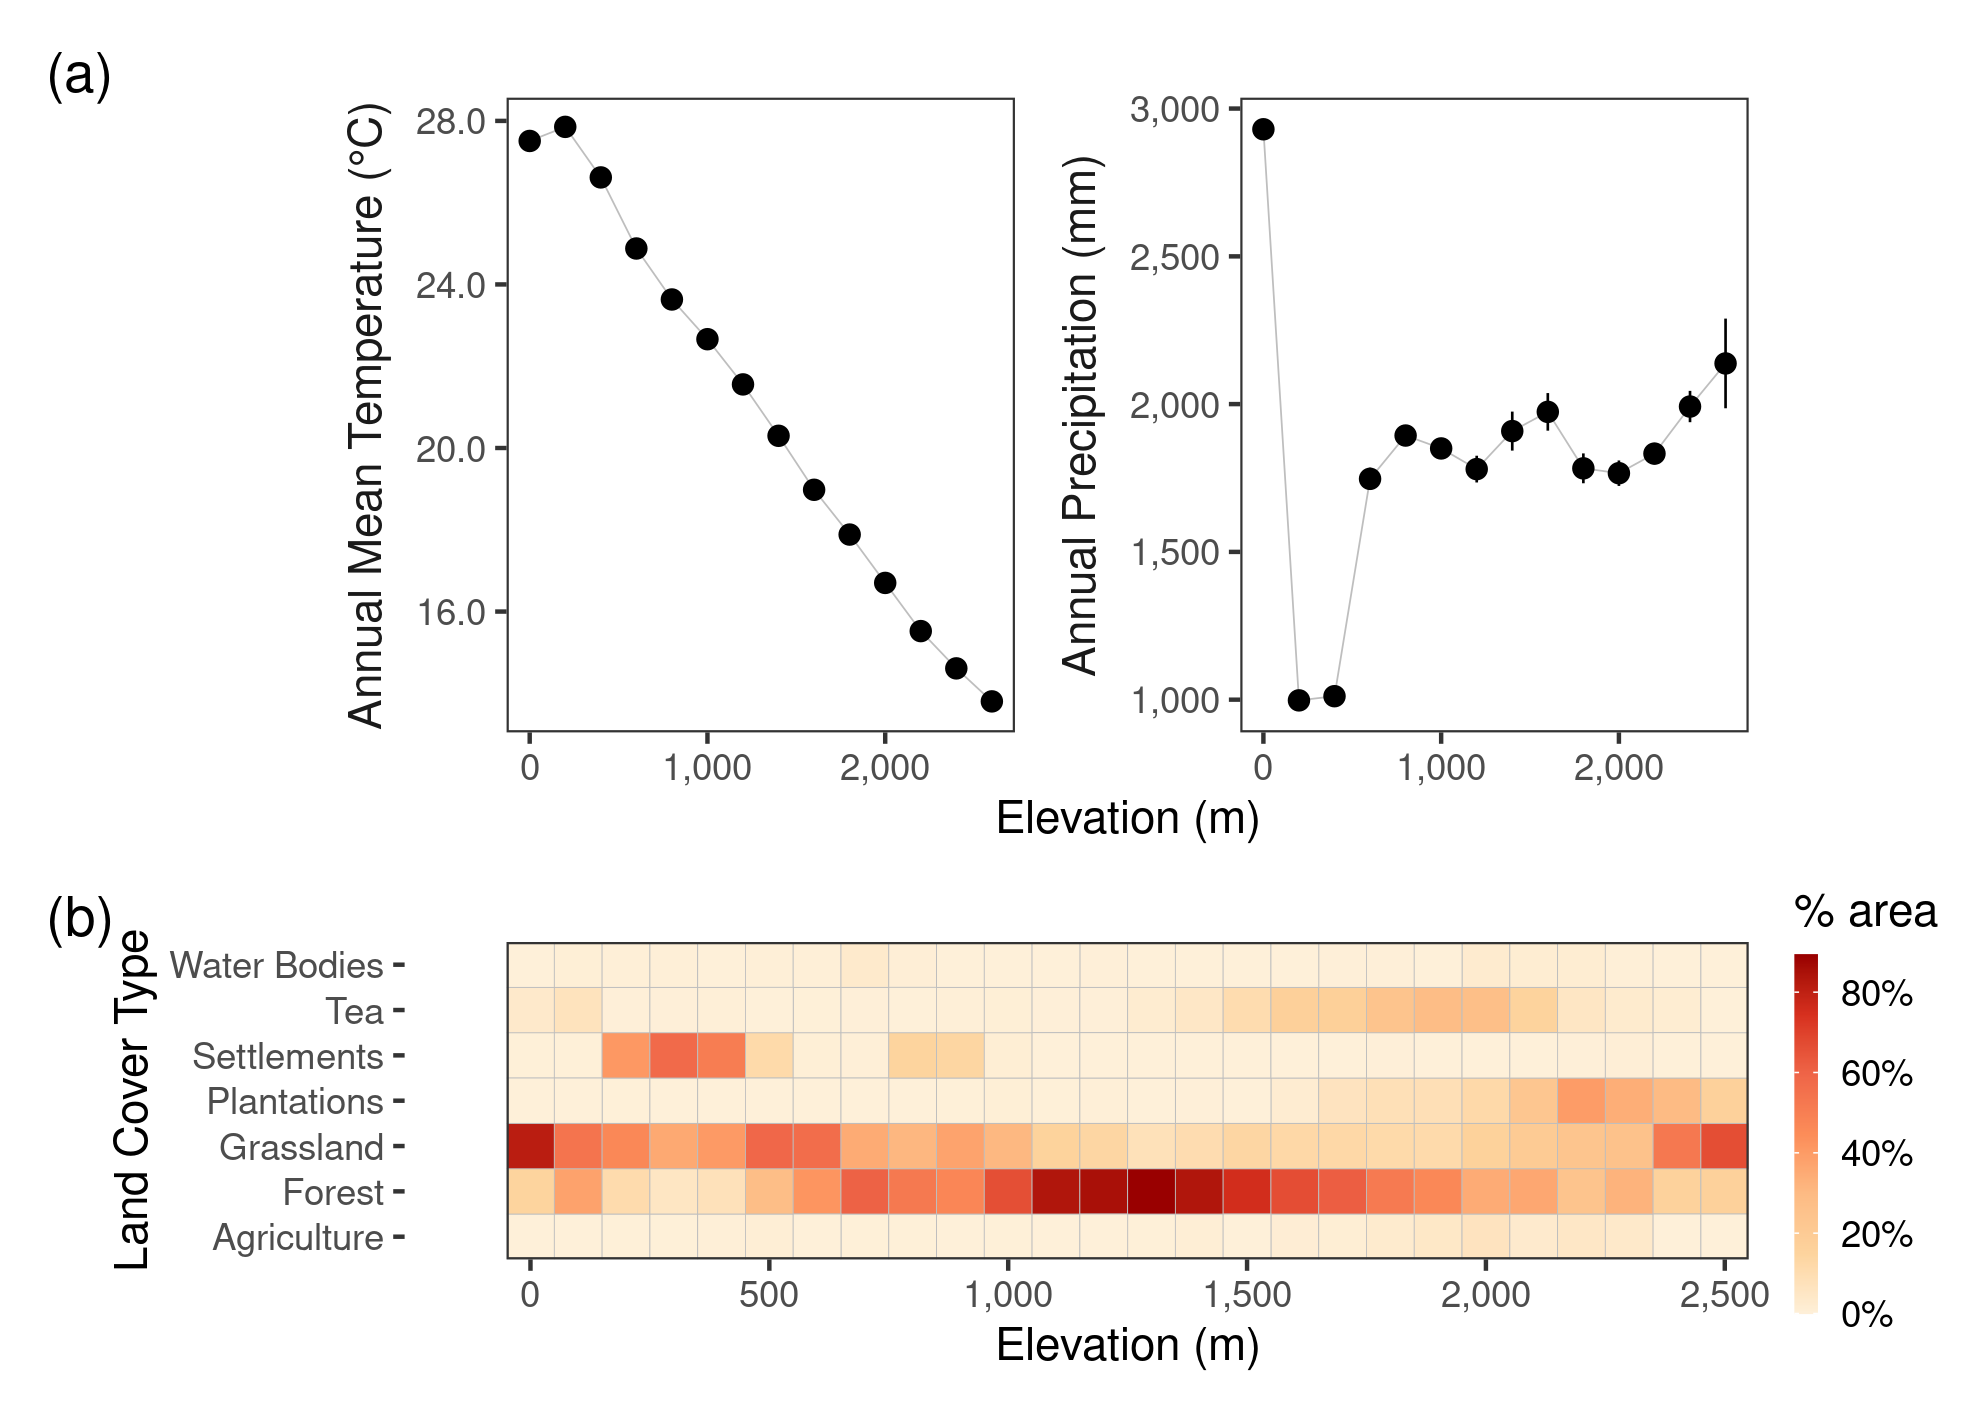
\includegraphics{figs/fig_02_clim_lc_elev.png}
\caption{Annual Mean Temperature varied from \textasciitilde{}28C in the plains to \textless{}14C at higher elevations. Annual precipitation increased at lower elevations (in the plains) to \textasciitilde{}3000mm and ranged between 1500mm and 2200mm at mid- and high elevations across the Nilgiri and the Anamalai hills. (b) The proportion of land cover types varied across the study area as shown in this panel (1 = agriculture; 2 = forest; 3 = grassland; 4 = plantations; 5 = settlements; 6 = tea; 7 = water bodies).}
\end{figure}

\hypertarget{examining-spatial-sampling-bias}{%
\section{Examining Spatial Sampling Bias}\label{examining-spatial-sampling-bias}}

The goal of this section is to determine how far each checklist location is from the nearest road, and how far each site is from its nearest neighbour. This involves finding the pairwise distance between a large number of unique checklist locations to a vast number of roads, as well as to each other.

Parts of this section are thus implemented in Python, using the R-Python interface package, \texttt{reticulate}.

\hypertarget{prepare-libraries-1}{%
\subsection{Prepare libraries}\label{prepare-libraries-1}}

\begin{Shaded}
\begin{Highlighting}[]
\CommentTok{# load libraries}
\KeywordTok{library}\NormalTok{(reticulate)}
\KeywordTok{library}\NormalTok{(sf)}
\KeywordTok{library}\NormalTok{(dplyr)}
\KeywordTok{library}\NormalTok{(scales)}
\KeywordTok{library}\NormalTok{(readr)}
\KeywordTok{library}\NormalTok{(purrr)}

\KeywordTok{library}\NormalTok{(ggplot2)}
\KeywordTok{library}\NormalTok{(ggthemes)}
\KeywordTok{library}\NormalTok{(ggspatial)}
\KeywordTok{library}\NormalTok{(scico)}

\CommentTok{# round any function}
\NormalTok{round_any <-}\StringTok{ }\ControlFlowTok{function}\NormalTok{(x, }\DataTypeTok{accuracy =} \DecValTok{20000}\NormalTok{) \{}
  \KeywordTok{round}\NormalTok{(x }\OperatorTok{/}\StringTok{ }\NormalTok{accuracy) }\OperatorTok{*}\StringTok{ }\NormalTok{accuracy}
\NormalTok{\}}
\CommentTok{# ci function}
\NormalTok{ci <-}\StringTok{ }\ControlFlowTok{function}\NormalTok{(x) \{}
  \KeywordTok{qnorm}\NormalTok{(}\FloatTok{0.975}\NormalTok{) }\OperatorTok{*}\StringTok{ }\KeywordTok{sd}\NormalTok{(x, }\DataTypeTok{na.rm =} \OtherTok{TRUE}\NormalTok{) }\OperatorTok{/}\StringTok{ }\KeywordTok{sqrt}\NormalTok{(}\KeywordTok{length}\NormalTok{(x))}
\NormalTok{\}}

\CommentTok{# set python path}
\KeywordTok{use_python}\NormalTok{(}\StringTok{"/usr/bin/python3"}\NormalTok{)}
\end{Highlighting}
\end{Shaded}

Importing python libraries. These libraries need to be installed before use.

\begin{Shaded}
\begin{Highlighting}[]
\CommentTok{# import classic python libs}
\ImportTok{import}\NormalTok{ itertools}
\ImportTok{from}\NormalTok{ operator }\ImportTok{import}\NormalTok{ itemgetter}
\ImportTok{import}\NormalTok{ numpy }\ImportTok{as}\NormalTok{ np}
\ImportTok{import}\NormalTok{ matplotlib.pyplot }\ImportTok{as}\NormalTok{ plt}
\ImportTok{import}\NormalTok{ math}

\CommentTok{# libs for dataframes}
\ImportTok{import}\NormalTok{ pandas }\ImportTok{as}\NormalTok{ pd}

\CommentTok{# import libs for geodata}
\ImportTok{from}\NormalTok{ shapely.ops }\ImportTok{import}\NormalTok{ nearest_points}
\ImportTok{import}\NormalTok{ geopandas }\ImportTok{as}\NormalTok{ gpd}
\ImportTok{import}\NormalTok{ rasterio}

\CommentTok{# import ckdtree}
\ImportTok{from}\NormalTok{ scipy.spatial }\ImportTok{import}\NormalTok{ cKDTree}
\ImportTok{from}\NormalTok{ shapely.geometry }\ImportTok{import}\NormalTok{ Point, MultiPoint, LineString, MultiLineString}
\end{Highlighting}
\end{Shaded}

\hypertarget{prepare-data-for-processing}{%
\subsection{Prepare data for processing}\label{prepare-data-for-processing}}

First we read in the roads shapefile, which is obtained from the Open Street Map database.
Then we read in the checklsit covariates, and extract the unique coordinate pairs.
All data are reprojected to be in the UTM 43N system.

We define a custom Python function to separate multi-feature geometries (here, roads which are in parts) into single feature geometries.
Then we define a function to use the K-dimensional trees method from \texttt{scipy} to find the distance between two geometries, here, the distance between the locations and the nearest road.
We define another function to find the distance between checklist locations and all other checklist locations.

We use these functions to find the distance between each checklist location and the nearest road and the next nearest site.

\hypertarget{python-functions-and-distance-calculations}{%
\subsubsection{Python functions and distance calculations}\label{python-functions-and-distance-calculations}}

\begin{Shaded}
\begin{Highlighting}[]
\CommentTok{# read in roads shapefile}
\NormalTok{roads }\OperatorTok{=}\NormalTok{ gpd.read_file(}\StringTok{"data/spatial/roads_studysite_2019/roads_studysite_2019.shp"}\NormalTok{)}
\NormalTok{roads.head()}

\CommentTok{# read in checklist covariates for conversion to gpd}
\CommentTok{# get unique coordinates, assign them to the df}
\CommentTok{# convert df to geo-df}
\NormalTok{chkCovars }\OperatorTok{=}\NormalTok{ pd.read_csv(}\StringTok{"data/eBirdChecklistVars.csv"}\NormalTok{)}
\NormalTok{unique_locs }\OperatorTok{=}\NormalTok{ chkCovars.drop_duplicates(subset}\OperatorTok{=}\NormalTok{[}\StringTok{'longitude'}\NormalTok{,}
                                         \StringTok{'latitude'}\NormalTok{])[[}\StringTok{'longitude'}\NormalTok{, }\StringTok{'latitude'}\NormalTok{]]}
\NormalTok{unique_locs[}\StringTok{'coordId'}\NormalTok{] }\OperatorTok{=}\NormalTok{ np.arange(}\DecValTok{1}\NormalTok{, unique_locs.shape[}\DecValTok{0}\NormalTok{]}\OperatorTok{+}\DecValTok{1}\NormalTok{)}
\NormalTok{chkCovars }\OperatorTok{=}\NormalTok{ chkCovars.merge(unique_locs, on}\OperatorTok{=}\NormalTok{[}\StringTok{'longitude'}\NormalTok{, }\StringTok{'latitude'}\NormalTok{])}

\NormalTok{unique_locs }\OperatorTok{=}\NormalTok{ gpd.GeoDataFrame(}
\NormalTok{unique_locs, }
\NormalTok{geometry }\OperatorTok{=}\NormalTok{ gpd.points_from_xy(unique_locs.longitude, unique_locs.latitude))}
\NormalTok{unique_locs.crs }\OperatorTok{=}\NormalTok{ \{}\StringTok{'init'}\NormalTok{ :}\StringTok{'epsg:4326'}\NormalTok{\}}

\CommentTok{# reproject spatials to 43n epsg 32643}

\NormalTok{roads }\OperatorTok{=}\NormalTok{ roads.to_crs(\{}\StringTok{'init'}\NormalTok{: }\StringTok{'epsg:32643'}\NormalTok{\})}
\NormalTok{unique_locs }\OperatorTok{=}\NormalTok{ unique_locs.to_crs(\{}\StringTok{'init'}\NormalTok{: }\StringTok{'epsg:32643'}\NormalTok{\})}


\CommentTok{# function to simplify multilinestrings}
\KeywordTok{def}\NormalTok{ simplify_roads(complex_roads):}
\NormalTok{    simpleRoads }\OperatorTok{=}\NormalTok{ []}
    \ControlFlowTok{for}\NormalTok{ i }\KeywordTok{in} \BuiltInTok{range}\NormalTok{(}\BuiltInTok{len}\NormalTok{(complex_roads.geometry)):}
\NormalTok{        feature }\OperatorTok{=}\NormalTok{ complex_roads.geometry.iloc[i]}
        \ControlFlowTok{if}\NormalTok{ feature.geom_type }\OperatorTok{==} \StringTok{"LineString"}\NormalTok{:}
\NormalTok{            simpleRoads.append(feature)}
        \ControlFlowTok{elif}\NormalTok{ feature.geom_type }\OperatorTok{==} \StringTok{"MultiLineString"}\NormalTok{:}
            \ControlFlowTok{for}\NormalTok{ road_level2 }\KeywordTok{in}\NormalTok{ feature:}
\NormalTok{                simpleRoads.append(road_level2)}
    \ControlFlowTok{return}\NormalTok{ simpleRoads}


\CommentTok{# function to use ckdtrees to find the nearest road}
\KeywordTok{def}\NormalTok{ ckdnearest(gdfA, gdfB):}
\NormalTok{    A }\OperatorTok{=}\NormalTok{ np.concatenate(}
\NormalTok{    [np.array(geom.coords) }\ControlFlowTok{for}\NormalTok{ geom }\KeywordTok{in}\NormalTok{ gdfA.geometry.to_list()])}
\NormalTok{    simplified_features }\OperatorTok{=}\NormalTok{ simplify_roads(gdfB)}
\NormalTok{    B }\OperatorTok{=}\NormalTok{ [np.array(geom.coords) }\ControlFlowTok{for}\NormalTok{ geom }\KeywordTok{in}\NormalTok{ simplified_features]}
\NormalTok{    B }\OperatorTok{=}\NormalTok{ np.concatenate(B)}
\NormalTok{    ckd_tree }\OperatorTok{=}\NormalTok{ cKDTree(B)}
\NormalTok{    dist, idx }\OperatorTok{=}\NormalTok{ ckd_tree.query(A, k}\OperatorTok{=}\DecValTok{1}\NormalTok{)}
    \ControlFlowTok{return}\NormalTok{ dist}


\CommentTok{# function to use ckdtrees for nearest other checklist point}
\KeywordTok{def}\NormalTok{ ckdnearest_point(gdfA, gdfB):}
\NormalTok{    A }\OperatorTok{=}\NormalTok{ np.concatenate(}
\NormalTok{    [np.array(geom.coords) }\ControlFlowTok{for}\NormalTok{ geom }\KeywordTok{in}\NormalTok{ gdfA.geometry.to_list()])}
    \CommentTok{#simplified_features = simplify_roads(gdfB)}
\NormalTok{    B }\OperatorTok{=}\NormalTok{ np.concatenate(}
\NormalTok{    [np.array(geom.coords) }\ControlFlowTok{for}\NormalTok{ geom }\KeywordTok{in}\NormalTok{ gdfB.geometry.to_list()])}
    \CommentTok{#B = np.concatenate(B)}
\NormalTok{    ckd_tree }\OperatorTok{=}\NormalTok{ cKDTree(B)}
\NormalTok{    dist, idx }\OperatorTok{=}\NormalTok{ ckd_tree.query(A, k}\OperatorTok{=}\NormalTok{[}\DecValTok{2}\NormalTok{])}
    \ControlFlowTok{return}\NormalTok{ dist}


\CommentTok{# get distance to nearest road}
\NormalTok{unique_locs[}\StringTok{'dist_road'}\NormalTok{] }\OperatorTok{=}\NormalTok{ ckdnearest(unique_locs, roads)}

\CommentTok{# get distance to nearest other site}
\NormalTok{unique_locs[}\StringTok{'nnb'}\NormalTok{] }\OperatorTok{=}\NormalTok{ ckdnearest_point(unique_locs, unique_locs)}

\CommentTok{# write to file}
\NormalTok{unique_locs }\OperatorTok{=}\NormalTok{ pd.DataFrame(unique_locs.drop(columns}\OperatorTok{=}\StringTok{'geometry'}\NormalTok{))}
\NormalTok{unique_locs[}\StringTok{'dist_road'}\NormalTok{] }\OperatorTok{=}\NormalTok{ unique_locs[}\StringTok{'dist_road'}\NormalTok{]}
\NormalTok{unique_locs[}\StringTok{'nnb'}\NormalTok{] }\OperatorTok{=}\NormalTok{ unique_locs[}\StringTok{'nnb'}\NormalTok{]}
\NormalTok{unique_locs.to_csv(path_or_buf }\OperatorTok{=} \StringTok{"data/locs_dist_to_road.csv"}\NormalTok{, index}\OperatorTok{=}\VariableTok{False}\NormalTok{)}

\CommentTok{# merge unique locs with chkCovars}
\NormalTok{chkCovars }\OperatorTok{=}\NormalTok{ chkCovars.merge(unique_locs, on}\OperatorTok{=}\NormalTok{[}\StringTok{'latitude'}\NormalTok{, }
                                             \StringTok{'longitude'}\NormalTok{, }\StringTok{'coordId'}\NormalTok{])}
\end{Highlighting}
\end{Shaded}

\hypertarget{spatially-explicit-filter-on-checklists}{%
\subsubsection{Spatially explicit filter on checklists}\label{spatially-explicit-filter-on-checklists}}

We filter the checklists by the boundary of the study area. This is \emph{not} the extent.

\begin{Shaded}
\begin{Highlighting}[]
\CommentTok{# extract data from python}
\NormalTok{chkCovars <-}\StringTok{ }\NormalTok{py}\OperatorTok{$}\NormalTok{chkCovars}
\NormalTok{chkCovars <-}\StringTok{ }\KeywordTok{st_as_sf}\NormalTok{(chkCovars, }\DataTypeTok{coords =} \KeywordTok{c}\NormalTok{(}\StringTok{"longitude"}\NormalTok{, }\StringTok{"latitude"}\NormalTok{)) }\OperatorTok
\StringTok{  `}\DataTypeTok{st_crs<-}\StringTok{`}\NormalTok{(}\DecValTok{4326}\NormalTok{) }\OperatorTok
\StringTok{  }\KeywordTok{st_transform}\NormalTok{(}\DecValTok{32643}\NormalTok{)}

\CommentTok{# read wg}
\NormalTok{wg <-}\StringTok{ }\KeywordTok{st_read}\NormalTok{(}\StringTok{"data/spatial/hillsShapefile/Nil_Ana_Pal.shp"}\NormalTok{) }\OperatorTok
\StringTok{  }\KeywordTok{st_transform}\NormalTok{(}\DecValTok{32643}\NormalTok{)}

\CommentTok{# spatial subset}
\NormalTok{chkCovars <-}\StringTok{ }\NormalTok{chkCovars }\OperatorTok
\StringTok{  }\KeywordTok{mutate}\NormalTok{(}\DataTypeTok{id =} \DecValTok{1}\OperatorTok{:}\KeywordTok{nrow}\NormalTok{(.)) }\OperatorTok
\StringTok{  }\KeywordTok{filter}\NormalTok{(id }\OperatorTok\StringTok{ }\KeywordTok{unlist}\NormalTok{(}\KeywordTok{st_contains}\NormalTok{(wg, chkCovars)))}
\end{Highlighting}
\end{Shaded}

\hypertarget{main-text-figure-3}{%
\subsection{Main Text Figure 3}\label{main-text-figure-3}}

\hypertarget{prepare-histogram-of-distance-to-roads}{%
\subsubsection{Prepare histogram of distance to roads}\label{prepare-histogram-of-distance-to-roads}}

Figure code is hidden in versions rendered as HTML or PDF.

\hypertarget{table-distance-to-roads}{%
\subsubsection{Table: Distance to roads}\label{table-distance-to-roads}}

\begin{Shaded}
\begin{Highlighting}[]
\CommentTok{# write the mean and ci95 to file}
\NormalTok{chkCovars }\OperatorTok
\StringTok{  }\KeywordTok{st_drop_geometry}\NormalTok{() }\OperatorTok
\StringTok{  }\KeywordTok{select}\NormalTok{(dist_road, nnb) }\OperatorTok
\StringTok{  }\NormalTok{tidyr}\OperatorTok{::}\KeywordTok{pivot_longer}\NormalTok{(}
    \DataTypeTok{cols =} \KeywordTok{c}\NormalTok{(}\StringTok{"dist_road"}\NormalTok{, }\StringTok{"nnb"}\NormalTok{),}
    \DataTypeTok{names_to =} \StringTok{"variable"}
\NormalTok{  ) }\OperatorTok
\StringTok{  }\KeywordTok{group_by}\NormalTok{(variable) }\OperatorTok
\StringTok{  }\KeywordTok{summarise_at}\NormalTok{(}
    \KeywordTok{vars}\NormalTok{(value),}
    \KeywordTok{list}\NormalTok{(}\OperatorTok{~}\StringTok{ }\KeywordTok{mean}\NormalTok{(.), }\OperatorTok{~}\StringTok{ }\KeywordTok{sd}\NormalTok{(.), }\OperatorTok{~}\StringTok{ }\KeywordTok{min}\NormalTok{(.), }\OperatorTok{~}\StringTok{ }\KeywordTok{max}\NormalTok{(.))}
\NormalTok{  ) }\OperatorTok
\StringTok{  }\KeywordTok{write_csv}\NormalTok{(}\StringTok{"data/results/distance_roads_sites.csv"}\NormalTok{)}
\end{Highlighting}
\end{Shaded}

\textbackslash{}begin\{table\}

\textbackslash{}caption\{(\#tab:show\_dist\_roads\_nnb)Distance to roads: Summary statistics\}
\centering

\begin{tabular}[t]{l|r|r|r|r}
\hline
variable & mean & sd & min & max\\
\hline
dist\_road & 390 & 859 & 0.279 & 7637\\
\hline
nnb & 297 & 553 & 0.137 & 12850\\
\hline
\end{tabular}

\textbackslash{}end\{table\}

\hypertarget{distance-to-nearest-neighbouring-site}{%
\subsection{Distance to nearest neighbouring site}\label{distance-to-nearest-neighbouring-site}}

\begin{Shaded}
\begin{Highlighting}[]
\CommentTok{# get unique locations}
\NormalTok{locs <-}\StringTok{ }\NormalTok{py}\OperatorTok{$}\NormalTok{unique_locs}
\end{Highlighting}
\end{Shaded}

Figure code is hidden in versions rendered as HTML and PDF.

\hypertarget{main-text-figure-3-1}{%
\subsection{Main Text Figure 3}\label{main-text-figure-3-1}}

\begin{Shaded}
\begin{Highlighting}[]
\NormalTok{roads <-}\StringTok{ }\KeywordTok{st_read}\NormalTok{(}\StringTok{"data/spatial/roads_studysite_2019/roads_studysite_2019.shp"}\NormalTok{) }\OperatorTok
\StringTok{  }\KeywordTok{st_transform}\NormalTok{(}\DecValTok{32643}\NormalTok{)}
\NormalTok{points <-}\StringTok{ }\NormalTok{chkCovars }\OperatorTok
\StringTok{  }\KeywordTok{bind_cols}\NormalTok{(}\KeywordTok{as_tibble}\NormalTok{(}\KeywordTok{st_coordinates}\NormalTok{(.))) }\OperatorTok
\StringTok{  }\KeywordTok{st_drop_geometry}\NormalTok{() }\OperatorTok
\StringTok{  }\KeywordTok{mutate}\NormalTok{(}\DataTypeTok{X =} \KeywordTok{round_any}\NormalTok{(X, }\DecValTok{2500}\NormalTok{), }\DataTypeTok{Y =} \KeywordTok{round_any}\NormalTok{(Y, }\DecValTok{2500}\NormalTok{))}

\NormalTok{points <-}\StringTok{ }\KeywordTok{count}\NormalTok{(points, X, Y)}

\CommentTok{# add land}
\KeywordTok{library}\NormalTok{(rnaturalearth)}
\NormalTok{land <-}\StringTok{ }\KeywordTok{ne_countries}\NormalTok{(}
  \DataTypeTok{scale =} \DecValTok{50}\NormalTok{, }\DataTypeTok{type =} \StringTok{"countries"}\NormalTok{, }\DataTypeTok{continent =} \StringTok{"asia"}\NormalTok{,}
  \DataTypeTok{country =} \StringTok{"india"}\NormalTok{,}
  \DataTypeTok{returnclass =} \KeywordTok{c}\NormalTok{(}\StringTok{"sf"}\NormalTok{)}
\NormalTok{) }\OperatorTok
\StringTok{  }\KeywordTok{st_transform}\NormalTok{(}\DecValTok{32643}\NormalTok{)}

\NormalTok{bbox <-}\StringTok{ }\KeywordTok{st_bbox}\NormalTok{(wg)}
\end{Highlighting}
\end{Shaded}

Figure code is hidden in versions rendered as HTML and PDF.

\begin{figure}
\centering
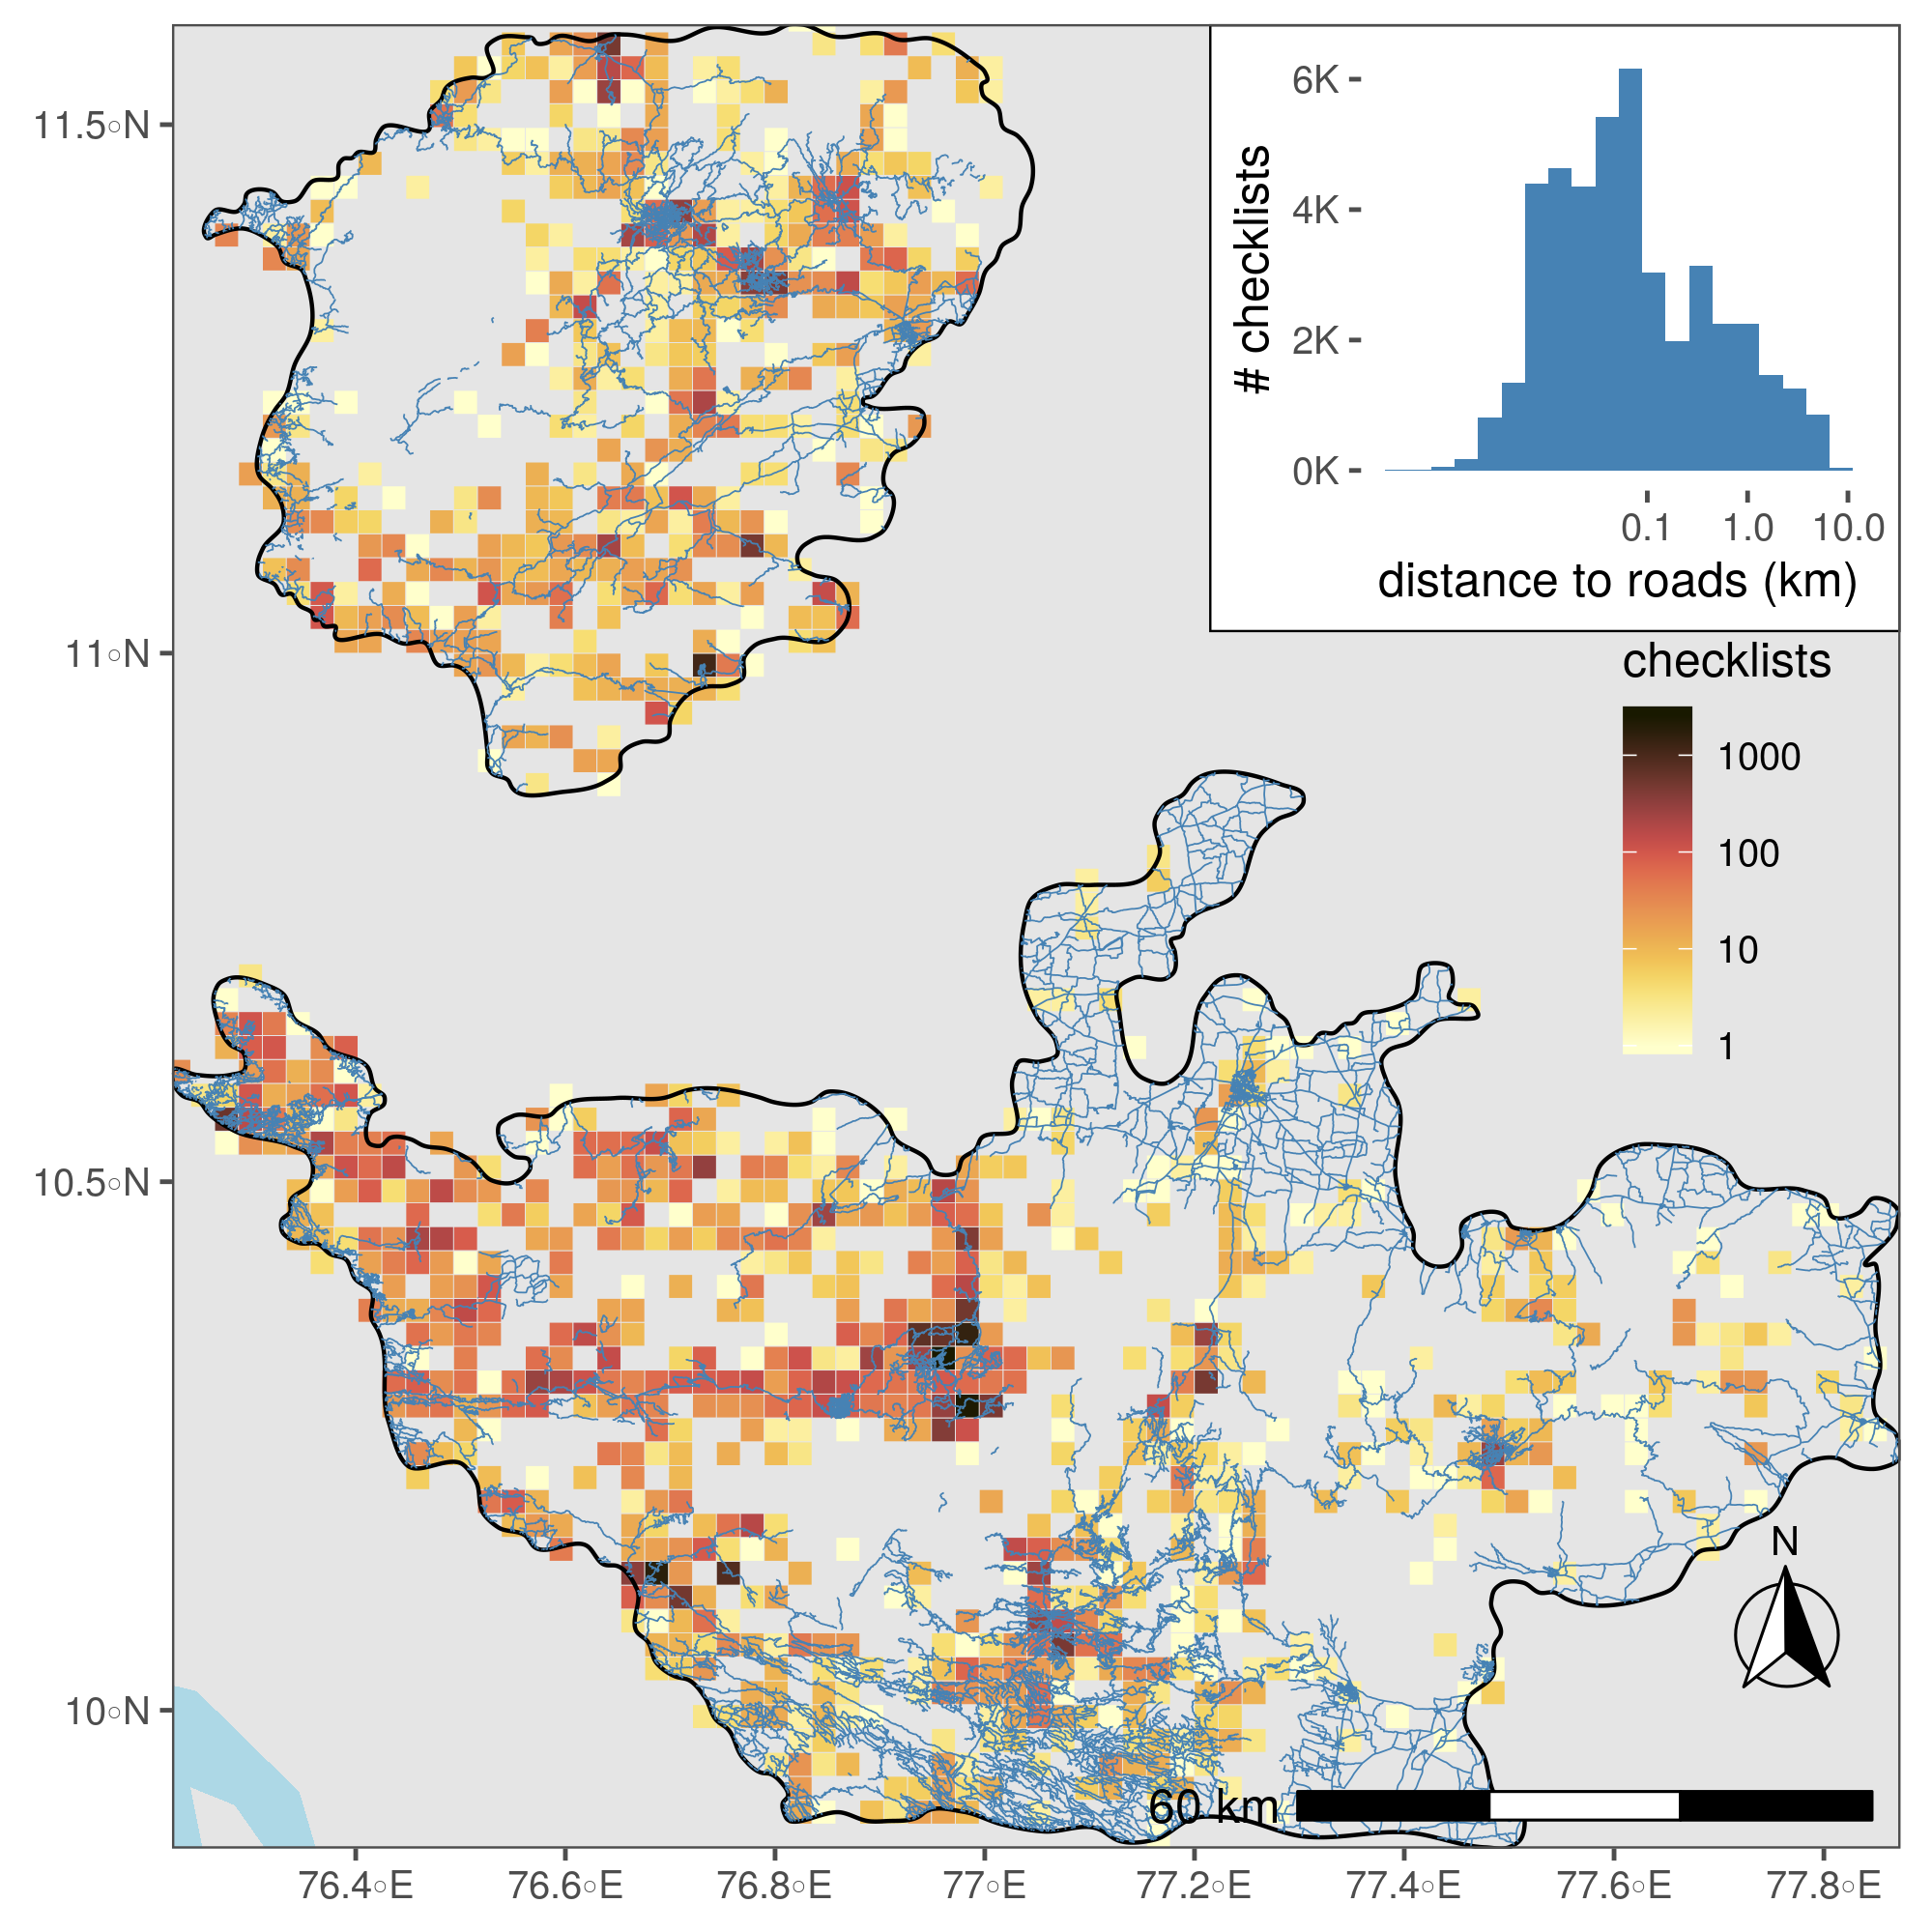
\includegraphics{figs/fig_03_distance_to_roads.png}
\caption{Spatial sampling bias of eBird observations across the Nilgiri and the Anamalai hills. A large proportion of localities/sites were next to roads and were on average only \textasciitilde{}300m from another locality/site.}
\end{figure}

\hypertarget{preparing-observer-expertise-scores}{%
\section{Preparing Observer Expertise Scores}\label{preparing-observer-expertise-scores}}

\hypertarget{prepare-libraries-2}{%
\subsection{Prepare libraries}\label{prepare-libraries-2}}

\begin{Shaded}
\begin{Highlighting}[]

\CommentTok{# load libs}
\KeywordTok{library}\NormalTok{(data.table)}
\KeywordTok{library}\NormalTok{(readxl)}
\KeywordTok{library}\NormalTok{(magrittr)}
\KeywordTok{library}\NormalTok{(stringr)}
\KeywordTok{library}\NormalTok{(dplyr)}
\KeywordTok{library}\NormalTok{(tidyr)}
\KeywordTok{library}\NormalTok{(auk)}

\CommentTok{# get decimal time function}
\KeywordTok{library}\NormalTok{(lubridate)}
\NormalTok{time_to_decimal <-}\StringTok{ }\ControlFlowTok{function}\NormalTok{(x) \{}
\NormalTok{  x <-}\StringTok{ }\NormalTok{lubridate}\OperatorTok{::}\KeywordTok{hms}\NormalTok{(x, }\DataTypeTok{quiet =} \OtherTok{TRUE}\NormalTok{)}
\NormalTok{  lubridate}\OperatorTok{::}\KeywordTok{hour}\NormalTok{(x) }\OperatorTok{+}\StringTok{ }\NormalTok{lubridate}\OperatorTok{::}\KeywordTok{minute}\NormalTok{(x) }\OperatorTok{/}\StringTok{ }\DecValTok{60} \OperatorTok{+}\StringTok{ }\NormalTok{lubridate}\OperatorTok{::}\KeywordTok{second}\NormalTok{(x) }\OperatorTok{/}\StringTok{ }\DecValTok{3600}
\NormalTok{\}}
\end{Highlighting}
\end{Shaded}

\hypertarget{prepare-data}{%
\subsection{Prepare data}\label{prepare-data}}

Here, we go through the data preparation process again because we might want to assess observer expertise over a larger area than the study site.

\begin{Shaded}
\begin{Highlighting}[]
\CommentTok{# Read in shapefile of study area to subset by bounding box}
\KeywordTok{library}\NormalTok{(sf)}
\NormalTok{wg <-}\StringTok{ }\KeywordTok{st_read}\NormalTok{(}\StringTok{"data/spatial/hillsShapefile/Nil_Ana_Pal.shp"}\NormalTok{) }\OperatorTok
\StringTok{  }\KeywordTok{st_transform}\NormalTok{(}\DecValTok{32643}\NormalTok{)}

\CommentTok{# set file paths for auk functions}
\NormalTok{f_in_ebd <-}\StringTok{ }\KeywordTok{file.path}\NormalTok{(}\StringTok{"data/eBirdDataWG_filtered.txt"}\NormalTok{)}
\NormalTok{f_in_sampling <-}\StringTok{ }\KeywordTok{file.path}\NormalTok{(}\StringTok{"data/eBirdSamplingDataWG_filtered.txt"}\NormalTok{)}

\CommentTok{# run filters using auk packages}
\NormalTok{ebd_filters <-}\StringTok{ }\KeywordTok{auk_ebd}\NormalTok{(f_in_ebd, f_in_sampling) }\OperatorTok
\StringTok{  }\KeywordTok{auk_country}\NormalTok{(}\DataTypeTok{country =} \StringTok{"IN"}\NormalTok{) }\OperatorTok
\StringTok{  }\KeywordTok{auk_state}\NormalTok{(}\KeywordTok{c}\NormalTok{(}\StringTok{"IN-KL"}\NormalTok{, }\StringTok{"IN-TN"}\NormalTok{, }\StringTok{"IN-KA"}\NormalTok{)) }\OperatorTok
\StringTok{  }\CommentTok{# Restricting geography to TamilNadu, Kerala & Karnataka}
\StringTok{  }\KeywordTok{auk_date}\NormalTok{(}\KeywordTok{c}\NormalTok{(}\StringTok{"2013-01-01"}\NormalTok{, }\StringTok{"2019-12-31"}\NormalTok{)) }\OperatorTok
\StringTok{  }\KeywordTok{auk_complete}\NormalTok{()}

\CommentTok{# check filters}
\NormalTok{ebd_filters}

\CommentTok{# specify output location and perform filter}
\NormalTok{f_out_ebd <-}\StringTok{ "data/ebird_for_expertise.txt"}
\NormalTok{f_out_sampling <-}\StringTok{ "data/ebird_sampling_for_expertise.txt"}

\NormalTok{ebd_filtered <-}\StringTok{ }\KeywordTok{auk_filter}\NormalTok{(ebd_filters,}
  \DataTypeTok{file =}\NormalTok{ f_out_ebd,}
  \DataTypeTok{file_sampling =}\NormalTok{ f_out_sampling, }\DataTypeTok{overwrite =} \OtherTok{TRUE}
\NormalTok{)}
\end{Highlighting}
\end{Shaded}

\begin{Shaded}
\begin{Highlighting}[]
\CommentTok{## Process filtered data}
\CommentTok{# read in the data}
\NormalTok{ebd <-}\StringTok{ }\KeywordTok{fread}\NormalTok{(f_out_ebd)}
\NormalTok{names <-}\StringTok{ }\KeywordTok{names}\NormalTok{(ebd) }\OperatorTok
\StringTok{  }\NormalTok{stringr}\OperatorTok{::}\KeywordTok{str_to_lower}\NormalTok{() }\OperatorTok
\StringTok{  }\NormalTok{stringr}\OperatorTok{::}\KeywordTok{str_replace_all}\NormalTok{(}\StringTok{" "}\NormalTok{, }\StringTok{"_"}\NormalTok{)}

\KeywordTok{setnames}\NormalTok{(ebd, names)}
\CommentTok{# choose columns of interest}
\NormalTok{columnsOfInterest <-}\StringTok{ }\KeywordTok{c}\NormalTok{(}
  \StringTok{"checklist_id"}\NormalTok{, }\StringTok{"scientific_name"}\NormalTok{, }\StringTok{"observation_count"}\NormalTok{,}
  \StringTok{"locality"}\NormalTok{, }\StringTok{"locality_id"}\NormalTok{, }\StringTok{"locality_type"}\NormalTok{, }\StringTok{"latitude"}\NormalTok{,}
  \StringTok{"longitude"}\NormalTok{, }\StringTok{"observation_date"}\NormalTok{,}
  \StringTok{"time_observations_started"}\NormalTok{, }\StringTok{"observer_id"}\NormalTok{,}
  \StringTok{"sampling_event_identifier"}\NormalTok{, }\StringTok{"protocol_type"}\NormalTok{,}
  \StringTok{"duration_minutes"}\NormalTok{, }\StringTok{"effort_distance_km"}\NormalTok{, }\StringTok{"effort_area_ha"}\NormalTok{,}
  \StringTok{"number_observers"}\NormalTok{, }\StringTok{"species_observed"}\NormalTok{, }\StringTok{"reviewed"}
\NormalTok{)}

\NormalTok{ebd <-}\StringTok{ }\KeywordTok{setDF}\NormalTok{(ebd) }\OperatorTok
\StringTok{  }\KeywordTok{as_tibble}\NormalTok{() }\OperatorTok
\StringTok{  }\NormalTok{dplyr}\OperatorTok{::}\KeywordTok{select}\NormalTok{(}\KeywordTok{one_of}\NormalTok{(columnsOfInterest))}

\KeywordTok{setDT}\NormalTok{(ebd)}
\end{Highlighting}
\end{Shaded}

\hypertarget{spatially-explicit-filter-on-checklists-1}{%
\subsection{Spatially explicit filter on checklists}\label{spatially-explicit-filter-on-checklists-1}}

\begin{Shaded}
\begin{Highlighting}[]
\CommentTok{# get checklist locations}
\NormalTok{ebd_locs <-}\StringTok{ }\NormalTok{ebd[, .(longitude, latitude)]}
\NormalTok{ebd_locs <-}\StringTok{ }\KeywordTok{setDF}\NormalTok{(ebd_locs) }\OperatorTok\StringTok{ }\KeywordTok{distinct}\NormalTok{()}
\NormalTok{ebd_locs <-}\StringTok{ }\KeywordTok{st_as_sf}\NormalTok{(ebd_locs,}
  \DataTypeTok{coords =} \KeywordTok{c}\NormalTok{(}\StringTok{"longitude"}\NormalTok{, }\StringTok{"latitude"}\NormalTok{)}
\NormalTok{) }\OperatorTok
\StringTok{  `}\DataTypeTok{st_crs<-}\StringTok{`}\NormalTok{(}\DecValTok{4326}\NormalTok{) }\OperatorTok
\StringTok{  }\KeywordTok{bind_cols}\NormalTok{(}\KeywordTok{as_tibble}\NormalTok{(}\KeywordTok{st_coordinates}\NormalTok{(.))) }\OperatorTok
\StringTok{  }\KeywordTok{st_transform}\NormalTok{(}\DecValTok{32643}\NormalTok{) }\OperatorTok
\StringTok{  }\KeywordTok{mutate}\NormalTok{(}\DataTypeTok{id =} \DecValTok{1}\OperatorTok{:}\KeywordTok{nrow}\NormalTok{(.))}

\CommentTok{# check whether to include}
\NormalTok{to_keep <-}\StringTok{ }\KeywordTok{unlist}\NormalTok{(}\KeywordTok{st_contains}\NormalTok{(wg, ebd_locs))}

\CommentTok{# filter locs}
\NormalTok{ebd_locs <-}\StringTok{ }\KeywordTok{filter}\NormalTok{(ebd_locs, id }\OperatorTok\StringTok{ }\NormalTok{to_keep) }\OperatorTok
\StringTok{  }\KeywordTok{bind_cols}\NormalTok{(}\KeywordTok{as_tibble}\NormalTok{(}\KeywordTok{st_coordinates}\NormalTok{(}\KeywordTok{st_as_sf}\NormalTok{(.)))) }\OperatorTok
\StringTok{  }\KeywordTok{st_drop_geometry}\NormalTok{()}
\end{Highlighting}
\end{Shaded}

\begin{Shaded}
\begin{Highlighting}[]
\NormalTok{ebd <-}\StringTok{ }\NormalTok{ebd[longitude }\OperatorTok\StringTok{ }\NormalTok{ebd_locs}\OperatorTok{$}\NormalTok{X }\OperatorTok{&}\StringTok{ }\NormalTok{latitude }\OperatorTok\StringTok{ }\NormalTok{ebd_locs}\OperatorTok{$}\NormalTok{Y, ]}
\end{Highlighting}
\end{Shaded}

\hypertarget{prepare-species-of-interest}{%
\subsection{Prepare species of interest}\label{prepare-species-of-interest}}

\begin{Shaded}
\begin{Highlighting}[]
\CommentTok{# read in species list}
\NormalTok{specieslist <-}\StringTok{ }\KeywordTok{read.csv}\NormalTok{(}\StringTok{"data/species_list.csv"}\NormalTok{)}

\CommentTok{# set species of interest}
\NormalTok{soi <-}\StringTok{ }\NormalTok{specieslist}\OperatorTok{$}\NormalTok{scientific_name}

\NormalTok{ebdSpSum <-}\StringTok{ }\NormalTok{ebd[, .(}
  \DataTypeTok{nSp =}\NormalTok{ .N,}
  \DataTypeTok{totSoiSeen =} \KeywordTok{length}\NormalTok{(}\KeywordTok{intersect}\NormalTok{(scientific_name, soi))}
\NormalTok{),}
\NormalTok{by =}\StringTok{ }\KeywordTok{list}\NormalTok{(sampling_event_identifier)}
\NormalTok{]}

\CommentTok{# write to file and link with checklsit id later}
\KeywordTok{fwrite}\NormalTok{(ebdSpSum, }\DataTypeTok{file =} \StringTok{"data/dataChecklistSpecies.csv"}\NormalTok{)}
\end{Highlighting}
\end{Shaded}

\hypertarget{prepare-checklists-for-observer-score}{%
\subsection{Prepare checklists for observer score}\label{prepare-checklists-for-observer-score}}

\begin{Shaded}
\begin{Highlighting}[]
\CommentTok{# 1. add new columns of decimal time and julian date}
\NormalTok{ebd[, }\StringTok{`}\DataTypeTok{:=}\StringTok{`}\NormalTok{(}
  \DataTypeTok{decimalTime =} \KeywordTok{time_to_decimal}\NormalTok{(time_observations_started),}
  \DataTypeTok{julianDate =} \KeywordTok{yday}\NormalTok{(}\KeywordTok{as.POSIXct}\NormalTok{(observation_date))}
\NormalTok{)]}

\NormalTok{ebdEffChk <-}\StringTok{ }\KeywordTok{setDF}\NormalTok{(ebd) }\OperatorTok
\StringTok{  }\KeywordTok{mutate}\NormalTok{(}\DataTypeTok{year =} \KeywordTok{year}\NormalTok{(observation_date)) }\OperatorTok
\StringTok{  }\KeywordTok{distinct}\NormalTok{(}
\NormalTok{    sampling_event_identifier, observer_id,}
\NormalTok{    year,}
\NormalTok{    duration_minutes, effort_distance_km, effort_area_ha,}
\NormalTok{    longitude, latitude,}
\NormalTok{    locality, locality_id,}
\NormalTok{    decimalTime, julianDate, number_observers}
\NormalTok{  ) }\OperatorTok
\StringTok{  }\CommentTok{# drop rows with NAs in cols used in the model}
\StringTok{  }\NormalTok{tidyr}\OperatorTok{::}\KeywordTok{drop_na}\NormalTok{(}
\NormalTok{    sampling_event_identifier, observer_id,}
\NormalTok{    duration_minutes, decimalTime, julianDate}
\NormalTok{  ) }\OperatorTok

\StringTok{  }\CommentTok{# drop years below 2013}
\StringTok{  }\KeywordTok{filter}\NormalTok{(year }\OperatorTok{>=}\StringTok{ }\DecValTok{2013}\NormalTok{)}

\CommentTok{# 3. join to covariates and remove large groups (> 10)}
\NormalTok{ebdChkSummary <-}\StringTok{ }\KeywordTok{inner_join}\NormalTok{(ebdEffChk, ebdSpSum)}

\CommentTok{# remove ebird data}
\KeywordTok{rm}\NormalTok{(ebd)}
\KeywordTok{gc}\NormalTok{()}
\end{Highlighting}
\end{Shaded}

\hypertarget{get-landcover}{%
\subsection{Get landcover}\label{get-landcover}}

Read in land cover type data resampled at 1km resolution.

\begin{Shaded}
\begin{Highlighting}[]
\CommentTok{# read in 1km landcover and set 0 to NA}
\KeywordTok{library}\NormalTok{(raster)}
\NormalTok{landcover <-}\StringTok{ }\NormalTok{raster}\OperatorTok{::}\KeywordTok{raster}\NormalTok{(}\StringTok{"data/landUseClassification/lc_01000m.tif"}\NormalTok{)}
\NormalTok{landcover[landcover }\OperatorTok{==}\StringTok{ }\DecValTok{0}\NormalTok{] <-}\StringTok{ }\OtherTok{NA}

\CommentTok{# get locs in utm coords}
\NormalTok{locs <-}\StringTok{ }\KeywordTok{distinct}\NormalTok{(}
\NormalTok{  ebdChkSummary, sampling_event_identifier, longitude, latitude,}
\NormalTok{  locality, locality_id}
\NormalTok{)}
\NormalTok{locs <-}\StringTok{ }\KeywordTok{st_as_sf}\NormalTok{(locs, }\DataTypeTok{coords =} \KeywordTok{c}\NormalTok{(}\StringTok{"longitude"}\NormalTok{, }\StringTok{"latitude"}\NormalTok{)) }\OperatorTok
\StringTok{  `}\DataTypeTok{st_crs<-}\StringTok{`}\NormalTok{(}\DecValTok{4326}\NormalTok{) }\OperatorTok
\StringTok{  }\KeywordTok{st_transform}\NormalTok{(}\DecValTok{32643}\NormalTok{) }\OperatorTok
\StringTok{  }\KeywordTok{st_coordinates}\NormalTok{()}

\CommentTok{# get for unique points}
\NormalTok{landcoverVec <-}\StringTok{ }\NormalTok{raster}\OperatorTok{::}\KeywordTok{extract}\NormalTok{(}
  \DataTypeTok{x =}\NormalTok{ landcover,}
  \DataTypeTok{y =}\NormalTok{ locs}
\NormalTok{)}

\CommentTok{# assign to df and overwrite}
\KeywordTok{setDT}\NormalTok{(ebdChkSummary)[, landcover }\OperatorTok{:}\ErrorTok{=}\StringTok{ }\NormalTok{landcoverVec]}
\end{Highlighting}
\end{Shaded}

\hypertarget{filter-checklist-data}{%
\subsection{Filter checklist data}\label{filter-checklist-data}}

\begin{Shaded}
\begin{Highlighting}[]
\CommentTok{# change names for easy handling}
\KeywordTok{setnames}\NormalTok{(ebdChkSummary, }\KeywordTok{c}\NormalTok{(}
  \StringTok{"sei"}\NormalTok{, }\StringTok{"observer"}\NormalTok{, }\StringTok{"year"}\NormalTok{, }\StringTok{"duration"}\NormalTok{, }\StringTok{"distance"}\NormalTok{,}
  \StringTok{"area"}\NormalTok{, }\StringTok{"longitude"}\NormalTok{, }\StringTok{"latitude"}\NormalTok{, }\StringTok{"locality"}\NormalTok{,}
  \StringTok{"locality_id"}\NormalTok{, }\StringTok{"decimalTime"}\NormalTok{,}
  \StringTok{"julianDate"}\NormalTok{, }\StringTok{"nObs"}\NormalTok{, }\StringTok{"nSp"}\NormalTok{, }\StringTok{"nSoi"}\NormalTok{, }\StringTok{"landcover"}
\NormalTok{))}

\CommentTok{# count data points per observer}
\NormalTok{obscount <-}\StringTok{ }\KeywordTok{count}\NormalTok{(ebdChkSummary, observer) }\OperatorTok
\StringTok{  }\KeywordTok{filter}\NormalTok{(n }\OperatorTok{>=}\StringTok{ }\DecValTok{10}\NormalTok{)}

\CommentTok{# make factor variables and remove obs not in obscount}
\CommentTok{# also remove 0 durations}
\NormalTok{ebdChkSummary <-}\StringTok{ }\NormalTok{ebdChkSummary }\OperatorTok
\StringTok{  }\KeywordTok{mutate}\NormalTok{(}
    \DataTypeTok{distance =} \KeywordTok{ifelse}\NormalTok{(}\KeywordTok{is.na}\NormalTok{(distance), }\DecValTok{0}\NormalTok{, distance),}
    \DataTypeTok{duration =} \KeywordTok{if_else}\NormalTok{(}\KeywordTok{is.na}\NormalTok{(duration), }\FloatTok{0.0}\NormalTok{, }\KeywordTok{as.double}\NormalTok{(duration))}
\NormalTok{  ) }\OperatorTok
\StringTok{  }\KeywordTok{filter}\NormalTok{(}
\NormalTok{    observer }\OperatorTok\StringTok{ }\NormalTok{obscount}\OperatorTok{$}\NormalTok{observer,}
\NormalTok{    duration }\OperatorTok{>}\StringTok{ }\DecValTok{0}\NormalTok{,}
\NormalTok{    duration }\OperatorTok{<=}\StringTok{ }\DecValTok{300}\NormalTok{,}
\NormalTok{    nSoi }\OperatorTok{>=}\StringTok{ }\DecValTok{0}\NormalTok{,}
\NormalTok{    distance }\OperatorTok{<=}\StringTok{ }\DecValTok{5}\NormalTok{,}
    \OperatorTok{!}\KeywordTok{is.na}\NormalTok{(nSoi)}
\NormalTok{  ) }\OperatorTok
\StringTok{  }\KeywordTok{mutate}\NormalTok{(}
    \DataTypeTok{landcover =} \KeywordTok{as.factor}\NormalTok{(landcover),}
    \DataTypeTok{observer =} \KeywordTok{as.factor}\NormalTok{(observer)}
\NormalTok{  ) }\OperatorTok
\StringTok{  }\KeywordTok{drop_na}\NormalTok{(landcover)}


\CommentTok{# save to file for later reuse}
\KeywordTok{fwrite}\NormalTok{(ebdChkSummary, }\DataTypeTok{file =} \StringTok{"data/eBirdChecklistVars.csv"}\NormalTok{)}
\end{Highlighting}
\end{Shaded}

\hypertarget{model-observer-expertise}{%
\subsection{Model observer expertise}\label{model-observer-expertise}}

Our observer expertise model aims to include the random intercept effect of observer identity, with a random slope effect of duration. This models the different rate of species accumulation by different observers, as well as their different starting points.

\begin{Shaded}
\begin{Highlighting}[]
\CommentTok{# uses either a subset or all data}
\KeywordTok{library}\NormalTok{(lmerTest)}

\CommentTok{# here we specify a glmm with random effects for observer}
\CommentTok{# time is considered a fixed log predictor and a random slope}
\NormalTok{modObsExp <-}\StringTok{ }\KeywordTok{glmer}\NormalTok{(nSoi }\OperatorTok{~}\StringTok{ }\KeywordTok{sqrt}\NormalTok{(duration) }\OperatorTok{+}
\StringTok{  }\NormalTok{landcover }\OperatorTok{+}
\StringTok{  }\KeywordTok{sqrt}\NormalTok{(decimalTime) }\OperatorTok{+}
\StringTok{  }\KeywordTok{I}\NormalTok{((}\KeywordTok{sqrt}\NormalTok{(decimalTime))}\OperatorTok{^}\DecValTok{2}\NormalTok{) }\OperatorTok{+}
\StringTok{  }\KeywordTok{log}\NormalTok{(julianDate) }\OperatorTok{+}
\StringTok{  }\KeywordTok{I}\NormalTok{((}\KeywordTok{log}\NormalTok{(julianDate)}\OperatorTok{^}\DecValTok{2}\NormalTok{)) }\OperatorTok{+}
\StringTok{  }\NormalTok{(}\DecValTok{1} \OperatorTok{|}\StringTok{ }\NormalTok{observer) }\OperatorTok{+}\StringTok{ }\NormalTok{(}\DecValTok{0} \OperatorTok{+}\StringTok{ }\NormalTok{duration }\OperatorTok{|}\StringTok{ }\NormalTok{observer),}
\DataTypeTok{data =}\NormalTok{ ebdChkSummary, }\DataTypeTok{family =} \StringTok{"poisson"}
\NormalTok{)}
\end{Highlighting}
\end{Shaded}

\begin{Shaded}
\begin{Highlighting}[]
\CommentTok{# make dir if absent}
\ControlFlowTok{if}\NormalTok{ (}\OperatorTok{!}\KeywordTok{dir.exists}\NormalTok{(}\StringTok{"data/modOutput"}\NormalTok{)) \{}
  \KeywordTok{dir.create}\NormalTok{(}\StringTok{"data/modOutput"}\NormalTok{)}
\NormalTok{\}}

\CommentTok{# write model output to text file}
\NormalTok{\{}
  \KeywordTok{writeLines}\NormalTok{(R.utils}\OperatorTok{::}\KeywordTok{captureOutput}\NormalTok{(}\KeywordTok{list}\NormalTok{(}\KeywordTok{Sys.time}\NormalTok{(), }\KeywordTok{summary}\NormalTok{(modObsExp))),}
    \DataTypeTok{con =} \StringTok{"data/modOutput/modOutExpertise.txt"}
\NormalTok{  )}
\NormalTok{\}}
\end{Highlighting}
\end{Shaded}

\begin{Shaded}
\begin{Highlighting}[]
\CommentTok{# make df with means}
\NormalTok{observer <-}\StringTok{ }\KeywordTok{unique}\NormalTok{(ebdChkSummary}\OperatorTok{$}\NormalTok{observer)}

\CommentTok{# predict at 60 mins on the most common landcover}
\NormalTok{dfPredict <-}\StringTok{ }\NormalTok{ebdChkSummary }\OperatorTok
\StringTok{  }\KeywordTok{summarise_at}\NormalTok{(}\KeywordTok{vars}\NormalTok{(duration, decimalTime, julianDate), }\KeywordTok{list}\NormalTok{(}\OperatorTok{~}\StringTok{ }\KeywordTok{mean}\NormalTok{(.))) }\OperatorTok
\StringTok{  }\KeywordTok{mutate}\NormalTok{(}\DataTypeTok{duration =} \DecValTok{60}\NormalTok{, }\DataTypeTok{landcover =} \KeywordTok{as.factor}\NormalTok{(}\DecValTok{6}\NormalTok{)) }\OperatorTok
\StringTok{  }\NormalTok{tidyr}\OperatorTok{::}\KeywordTok{crossing}\NormalTok{(observer)}

\CommentTok{# run predict from model on it}
\NormalTok{dfPredict <-}\StringTok{ }\KeywordTok{mutate}\NormalTok{(dfPredict,}
  \DataTypeTok{score =} \KeywordTok{predict}\NormalTok{(modObsExp,}
    \DataTypeTok{newdata =}\NormalTok{ dfPredict,}
    \DataTypeTok{type =} \StringTok{"response"}\NormalTok{,}
    \DataTypeTok{allow.new.levels =} \OtherTok{TRUE}
\NormalTok{  )}
\NormalTok{) }\OperatorTok
\StringTok{  }\KeywordTok{mutate}\NormalTok{(}\DataTypeTok{score =}\NormalTok{ scales}\OperatorTok{::}\KeywordTok{rescale}\NormalTok{(score))}
\end{Highlighting}
\end{Shaded}

\begin{Shaded}
\begin{Highlighting}[]
\KeywordTok{fwrite}\NormalTok{(dfPredict }\OperatorTok\StringTok{ }\NormalTok{dplyr}\OperatorTok{::}\KeywordTok{select}\NormalTok{(observer, score),}
  \DataTypeTok{file =} \StringTok{"data/dataObsExpScore.csv"}
\NormalTok{)}
\end{Highlighting}
\end{Shaded}

\hypertarget{adding-covariates-to-checklist-data}{%
\section{Adding Covariates to Checklist Data}\label{adding-covariates-to-checklist-data}}

\hypertarget{prepare-libraries-and-data}{%
\subsection{Prepare libraries and data}\label{prepare-libraries-and-data}}

\begin{Shaded}
\begin{Highlighting}[]

\CommentTok{# load libs}
\KeywordTok{library}\NormalTok{(dplyr)}
\KeywordTok{library}\NormalTok{(readr)}
\KeywordTok{library}\NormalTok{(stringr)}
\KeywordTok{library}\NormalTok{(purrr)}
\KeywordTok{library}\NormalTok{(raster)}
\KeywordTok{library}\NormalTok{(glue)}
\KeywordTok{library}\NormalTok{(velox)}
\KeywordTok{library}\NormalTok{(tidyr)}
\KeywordTok{library}\NormalTok{(sf)}

\CommentTok{# load saved data object}
\KeywordTok{load}\NormalTok{(}\StringTok{"data/data_prelim_processing.rdata"}\NormalTok{)}
\end{Highlighting}
\end{Shaded}

\hypertarget{spatial-subsampling}{%
\subsection{Spatial subsampling}\label{spatial-subsampling}}

\begin{Shaded}
\begin{Highlighting}[]
\CommentTok{# grid based spatial thinning}
\NormalTok{gridsize <-}\StringTok{ }\DecValTok{1000} \CommentTok{# grid size in metres}
\NormalTok{effort_distance_max <-}\StringTok{ }\DecValTok{1000} \CommentTok{# removing checklists with this distance}

\CommentTok{# make grids across the study site}
\NormalTok{hills <-}\StringTok{ }\KeywordTok{st_read}\NormalTok{(}\StringTok{"data/spatial/hillsShapefile/Nil_Ana_Pal.shp"}\NormalTok{) }\OperatorTok
\StringTok{  }\KeywordTok{st_transform}\NormalTok{(}\DecValTok{32643}\NormalTok{)}
\NormalTok{grid <-}\StringTok{ }\KeywordTok{st_make_grid}\NormalTok{(hills, }\DataTypeTok{cellsize =}\NormalTok{ gridsize)}

\CommentTok{# split data by species}
\NormalTok{data_spatial_thin <-}\StringTok{ }\KeywordTok{split}\NormalTok{(}\DataTypeTok{x =}\NormalTok{ dataGrouped, }\DataTypeTok{f =}\NormalTok{ dataGrouped}\OperatorTok{$}\NormalTok{scientific_name)}

\CommentTok{# spatial thinning on each species retains}
\CommentTok{# site with maximum visits per grid cell}
\NormalTok{data_spatial_thin <-}\StringTok{ }\KeywordTok{map}\NormalTok{(data_spatial_thin, }\ControlFlowTok{function}\NormalTok{(df) \{}

  \CommentTok{# count visits per locality}
\NormalTok{  df <-}\StringTok{ }\KeywordTok{group_by}\NormalTok{(df, locality) }\OperatorTok
\StringTok{    }\KeywordTok{mutate}\NormalTok{(}\DataTypeTok{tot_effort =} \KeywordTok{length}\NormalTok{(sampling_event_identifier)) }\OperatorTok
\StringTok{    }\KeywordTok{ungroup}\NormalTok{()}

  \CommentTok{# remove sites with distances above spatial independence}
\NormalTok{  df <-}\StringTok{ }\NormalTok{df }\OperatorTok
\StringTok{    }\KeywordTok{filter}\NormalTok{(effort_distance_km }\OperatorTok{<=}\StringTok{ }\NormalTok{effort_distance_max) }\OperatorTok
\StringTok{    }\KeywordTok{st_as_sf}\NormalTok{(}\DataTypeTok{coords =} \KeywordTok{c}\NormalTok{(}\StringTok{"longitude"}\NormalTok{, }\StringTok{"latitude"}\NormalTok{)) }\OperatorTok
\StringTok{    `}\DataTypeTok{st_crs<-}\StringTok{`}\NormalTok{(}\DecValTok{4326}\NormalTok{) }\OperatorTok
\StringTok{    }\KeywordTok{st_transform}\NormalTok{(}\DecValTok{32643}\NormalTok{) }\OperatorTok
\StringTok{    }\KeywordTok{mutate}\NormalTok{(}\DataTypeTok{coordId =} \DecValTok{1}\OperatorTok{:}\KeywordTok{nrow}\NormalTok{(.)) }\OperatorTok
\StringTok{    }\KeywordTok{bind_cols}\NormalTok{(}\KeywordTok{as_tibble}\NormalTok{(}\KeywordTok{st_coordinates}\NormalTok{(.)))}

  \CommentTok{# whcih cell has which coords}
\NormalTok{  grid_contents <-}\StringTok{ }\KeywordTok{st_contains}\NormalTok{(grid, df) }\OperatorTok
\StringTok{    }\KeywordTok{as_tibble}\NormalTok{() }\OperatorTok
\StringTok{    }\KeywordTok{rename}\NormalTok{(}\DataTypeTok{cell =}\NormalTok{ row.id, }\DataTypeTok{coordId =}\NormalTok{ col.id)}

  \CommentTok{# what's the max point in each grid}
\NormalTok{  points_max <-}\StringTok{ }\KeywordTok{left_join}\NormalTok{(df }\OperatorTok\StringTok{ }\KeywordTok{st_drop_geometry}\NormalTok{(),}
\NormalTok{    grid_contents,}
    \DataTypeTok{by =} \StringTok{"coordId"}
\NormalTok{  ) }\OperatorTok
\StringTok{    }\KeywordTok{group_by}\NormalTok{(cell) }\OperatorTok
\StringTok{    }\KeywordTok{filter}\NormalTok{(tot_effort }\OperatorTok{==}\StringTok{ }\KeywordTok{max}\NormalTok{(tot_effort))}

  \KeywordTok{return}\NormalTok{(points_max)}
\NormalTok{\})}

\CommentTok{# remove old data}
\KeywordTok{rm}\NormalTok{(dataGrouped)}
\end{Highlighting}
\end{Shaded}

\hypertarget{temporal-subsampling}{%
\subsection{Temporal subsampling}\label{temporal-subsampling}}

Get 10 random (if available) observations of each species at each locality.

\begin{Shaded}
\begin{Highlighting}[]
\CommentTok{# subsample data for random 10 observations}
\NormalTok{dataSubsample <-}\StringTok{ }\KeywordTok{map}\NormalTok{(data_spatial_thin, }\ControlFlowTok{function}\NormalTok{(df) \{}
\NormalTok{  df <-}\StringTok{ }\KeywordTok{ungroup}\NormalTok{(df)}
\NormalTok{  df_to_locality <-}\StringTok{ }\KeywordTok{split}\NormalTok{(}\DataTypeTok{x =}\NormalTok{ df, }\DataTypeTok{f =}\NormalTok{ df}\OperatorTok{$}\NormalTok{locality)}
\NormalTok{  df_samples <-}\StringTok{ }\KeywordTok{map_if}\NormalTok{(}
    \DataTypeTok{.x =}\NormalTok{ df_to_locality,}
    \DataTypeTok{.p =} \ControlFlowTok{function}\NormalTok{(x) \{}
      \KeywordTok{nrow}\NormalTok{(x) }\OperatorTok{>}\StringTok{ }\DecValTok{10}
\NormalTok{    \},}
    \DataTypeTok{.f =} \ControlFlowTok{function}\NormalTok{(x) }\KeywordTok{sample_n}\NormalTok{(x, }\DecValTok{10}\NormalTok{, }\DataTypeTok{replace =} \OtherTok{FALSE}\NormalTok{)}
\NormalTok{  )}

  \KeywordTok{return}\NormalTok{(}\KeywordTok{bind_rows}\NormalTok{(df_samples))}
\NormalTok{\})}

\CommentTok{# bind all rows for data frame}
\NormalTok{dataSubsample <-}\StringTok{ }\KeywordTok{bind_rows}\NormalTok{(dataSubsample)}

\CommentTok{# remove previous data}
\KeywordTok{rm}\NormalTok{(data_spatial_thin)}
\end{Highlighting}
\end{Shaded}

\hypertarget{add-checklist-calibration-index}{%
\subsection{Add checklist calibration index}\label{add-checklist-calibration-index}}

\begin{Shaded}
\begin{Highlighting}[]
\CommentTok{# read in obs score and extract numbers}
\NormalTok{expertiseScore <-}\StringTok{ }\KeywordTok{read_csv}\NormalTok{(}\StringTok{"data/dataObsExpScore.csv"}\NormalTok{) }\OperatorTok
\StringTok{  }\KeywordTok{mutate}\NormalTok{(}\DataTypeTok{numObserver =} \KeywordTok{str_extract}\NormalTok{(observer, }\StringTok{"}\CharTok{\textbackslash{}\textbackslash{}}\StringTok{d+"}\NormalTok{)) }\OperatorTok
\StringTok{  }\NormalTok{dplyr}\OperatorTok{::}\KeywordTok{select}\NormalTok{(}\OperatorTok{-}\NormalTok{observer)}

\CommentTok{# group seis consist of multiple observers}
\CommentTok{# in this case, seis need to have the highest expertise observer score}
\CommentTok{# as the associated covariate}

\CommentTok{# get unique observers per sei}
\NormalTok{dataSeiScore <-}\StringTok{ }\KeywordTok{distinct}\NormalTok{(}
\NormalTok{  dataSubsample, sampling_event_identifier,}
\NormalTok{  observer_id}
\NormalTok{) }\OperatorTok
\StringTok{  }\CommentTok{# make list column of observers}
\StringTok{  }\KeywordTok{mutate}\NormalTok{(}\DataTypeTok{observers =} \KeywordTok{str_split}\NormalTok{(observer_id, }\StringTok{","}\NormalTok{)) }\OperatorTok
\StringTok{  }\KeywordTok{unnest}\NormalTok{(}\DataTypeTok{cols =} \KeywordTok{c}\NormalTok{(observers)) }\OperatorTok
\StringTok{  }\CommentTok{# add numeric observer id}
\StringTok{  }\KeywordTok{mutate}\NormalTok{(}\DataTypeTok{numObserver =} \KeywordTok{str_extract}\NormalTok{(observers, }\StringTok{"}\CharTok{\textbackslash{}\textbackslash{}}\StringTok{d+"}\NormalTok{)) }\OperatorTok
\StringTok{  }\CommentTok{# now get distinct sei and observer id numeric}
\StringTok{  }\KeywordTok{distinct}\NormalTok{(sampling_event_identifier, numObserver)}

\CommentTok{# now add expertise score to sei}
\NormalTok{dataSeiScore <-}\StringTok{ }\KeywordTok{left_join}\NormalTok{(dataSeiScore, expertiseScore,}
  \DataTypeTok{by =} \StringTok{"numObserver"}
\NormalTok{) }\OperatorTok
\StringTok{  }\CommentTok{# get max expertise score per sei}
\StringTok{  }\KeywordTok{group_by}\NormalTok{(sampling_event_identifier) }\OperatorTok
\StringTok{  }\KeywordTok{summarise}\NormalTok{(}\DataTypeTok{expertise =} \KeywordTok{max}\NormalTok{(score))}

\CommentTok{# add to dataCovar}
\NormalTok{dataSubsample <-}\StringTok{ }\KeywordTok{left_join}\NormalTok{(dataSubsample, dataSeiScore,}
  \DataTypeTok{by =} \StringTok{"sampling_event_identifier"}
\NormalTok{)}

\CommentTok{# remove data without expertise score}
\NormalTok{dataSubsample <-}\StringTok{ }\KeywordTok{filter}\NormalTok{(dataSubsample, }\OperatorTok{!}\KeywordTok{is.na}\NormalTok{(expertise))}
\end{Highlighting}
\end{Shaded}

\hypertarget{add-landscape-covariates}{%
\subsection{Add landscape covariates}\label{add-landscape-covariates}}

\begin{Shaded}
\begin{Highlighting}[]

\CommentTok{# list landscape covariate stacks}
\NormalTok{landscape_files <-}\StringTok{ "data/landcover}\CharTok{\textbackslash{}\textbackslash{}}\StringTok{landscape_resamp01km.tif"}

\CommentTok{# read in as stacks}
\NormalTok{landscape_data <-}\StringTok{ }\KeywordTok{stack}\NormalTok{(landscape_files)}

\CommentTok{# get proper names}
\NormalTok{elev_names <-}\StringTok{ }\KeywordTok{c}\NormalTok{(}\StringTok{"elev"}\NormalTok{, }\StringTok{"slope"}\NormalTok{, }\StringTok{"aspect"}\NormalTok{)}
\NormalTok{chelsa_names <-}\StringTok{ }\KeywordTok{c}\NormalTok{(}\StringTok{"bio1"}\NormalTok{,}\StringTok{"bio12"}\NormalTok{)}

\KeywordTok{names}\NormalTok{(landscape_data) <-}\StringTok{ }\KeywordTok{as.character}\NormalTok{(}\KeywordTok{glue}\NormalTok{(}\StringTok{'\{c(elev_names, chelsa_names, "landcover")\}'}\NormalTok{))}
\end{Highlighting}
\end{Shaded}

\hypertarget{spatial-buffers-around-selected-checklists}{%
\subsection{Spatial buffers around selected checklists}\label{spatial-buffers-around-selected-checklists}}

\begin{Shaded}
\begin{Highlighting}[]
\CommentTok{# assign neighbourhood radius in m}
\NormalTok{sample_radius <-}\StringTok{ }\FloatTok{2.5} \OperatorTok{*}\StringTok{ }\FloatTok{1e3}

\CommentTok{# get distinct points and make buffer}
\NormalTok{ebird_buff <-}\StringTok{ }\NormalTok{dataSubsample }\OperatorTok
\StringTok{  }\KeywordTok{ungroup}\NormalTok{() }\OperatorTok
\StringTok{  }\KeywordTok{distinct}\NormalTok{(X, Y) }\OperatorTok
\StringTok{  }\KeywordTok{mutate}\NormalTok{(}\DataTypeTok{id =} \DecValTok{1}\OperatorTok{:}\KeywordTok{nrow}\NormalTok{(.)) }\OperatorTok
\StringTok{  }\KeywordTok{crossing}\NormalTok{(sample_radius) }\OperatorTok
\StringTok{  }\KeywordTok{arrange}\NormalTok{(id) }\OperatorTok
\StringTok{  }\KeywordTok{group_by}\NormalTok{(sample_radius) }\OperatorTok
\StringTok{  }\KeywordTok{nest}\NormalTok{() }\OperatorTok
\StringTok{  }\KeywordTok{ungroup}\NormalTok{()}


\CommentTok{# convert to spatial features}
\NormalTok{ebird_buff <-}\StringTok{ }\KeywordTok{mutate}\NormalTok{(ebird_buff,}
  \DataTypeTok{data =} \KeywordTok{map2}\NormalTok{(}
\NormalTok{    data, sample_radius,}
    \ControlFlowTok{function}\NormalTok{(df, rd) \{}
\NormalTok{      df_sf <-}\StringTok{ }\KeywordTok{st_as_sf}\NormalTok{(df, }\DataTypeTok{coords =} \KeywordTok{c}\NormalTok{(}\StringTok{"X"}\NormalTok{, }\StringTok{"Y"}\NormalTok{), }\DataTypeTok{crs =} \DecValTok{32643}\NormalTok{) }\OperatorTok
\StringTok{        }\CommentTok{# add long lat}
\StringTok{        }\KeywordTok{bind_cols}\NormalTok{(}\KeywordTok{as_tibble}\NormalTok{(}\KeywordTok{st_coordinates}\NormalTok{(.))) }\OperatorTok
\StringTok{        }\CommentTok{# rename(longitude = X, latitude = Y) %>%}
\StringTok{        }\CommentTok{# # transform to modis projection}
\StringTok{        }\CommentTok{# st_transform(crs = 32643) %>%}
\StringTok{        }\CommentTok{# buffer to create neighborhood around each point}
\StringTok{        }\KeywordTok{st_buffer}\NormalTok{(}\DataTypeTok{dist =}\NormalTok{ rd)}
\NormalTok{    \}}
\NormalTok{  )}
\NormalTok{)}
\end{Highlighting}
\end{Shaded}

\hypertarget{spatial-buffer-wide-covariates}{%
\subsection{Spatial buffer-wide covariates}\label{spatial-buffer-wide-covariates}}

\hypertarget{mean-environmental-covariates}{%
\subsubsection{Mean environmental covariates}\label{mean-environmental-covariates}}

All covariates are 2.5km mean values and prefixed ``am\_''.

\begin{Shaded}
\begin{Highlighting}[]
\CommentTok{# get area mean for all preds except landcover, which is the last one}
\NormalTok{env_area_mean <-}\StringTok{ }\NormalTok{purrr}\OperatorTok{::}\KeywordTok{map}\NormalTok{(ebird_buff}\OperatorTok{$}\NormalTok{data, }\ControlFlowTok{function}\NormalTok{(df) \{}
\NormalTok{  stk <-}\StringTok{ }\NormalTok{landscape_data[[}\OperatorTok{-}\KeywordTok{dim}\NormalTok{(landscape_data)[}\DecValTok{3}\NormalTok{]]] }\CommentTok{# removing landcover here}
\NormalTok{  velstk <-}\StringTok{ }\KeywordTok{velox}\NormalTok{(stk)}
\NormalTok{  dextr <-}\StringTok{ }\NormalTok{velstk}\OperatorTok{$}\KeywordTok{extract}\NormalTok{(}
    \DataTypeTok{sp =}\NormalTok{ df, }\DataTypeTok{df =} \OtherTok{TRUE}\NormalTok{,}
    \DataTypeTok{fun =} \ControlFlowTok{function}\NormalTok{(x) }\KeywordTok{mean}\NormalTok{(x, }\DataTypeTok{na.rm =}\NormalTok{ T)}
\NormalTok{  )}

  \CommentTok{# assign names for joining}
  \KeywordTok{names}\NormalTok{(dextr) <-}\StringTok{ }\KeywordTok{c}\NormalTok{(}\StringTok{"id"}\NormalTok{, }\KeywordTok{names}\NormalTok{(stk))}
  \KeywordTok{return}\NormalTok{(}\KeywordTok{as_tibble}\NormalTok{(dextr))}
\NormalTok{\})}

\CommentTok{# join to buffer data}
\NormalTok{ebird_buff <-}\StringTok{ }\NormalTok{ebird_buff }\OperatorTok
\StringTok{  }\KeywordTok{mutate}\NormalTok{(}\DataTypeTok{data =} \KeywordTok{map2}\NormalTok{(data, env_area_mean, inner_join, }\DataTypeTok{by =} \StringTok{"id"}\NormalTok{))}
\end{Highlighting}
\end{Shaded}

\hypertarget{proportions-of-land-cover-type}{%
\subsubsection{Proportions of land cover type}\label{proportions-of-land-cover-type}}

\begin{Shaded}
\begin{Highlighting}[]
\CommentTok{# get the last element of each stack from the list}
\CommentTok{# this is the landcover at that resolution}
\NormalTok{lc_area_prop <-}\StringTok{ }\NormalTok{purrr}\OperatorTok{::}\KeywordTok{map}\NormalTok{(ebird_buff}\OperatorTok{$}\NormalTok{data, }\ControlFlowTok{function}\NormalTok{(df) \{}
\NormalTok{  lc <-}\StringTok{ }\NormalTok{landscape_data[[}\KeywordTok{dim}\NormalTok{(landscape_data)[}\DecValTok{3}\NormalTok{]]] }\CommentTok{# accessing landcover here}
\NormalTok{  lc_velox <-}\StringTok{ }\KeywordTok{velox}\NormalTok{(lc)}
\NormalTok{  lc_vals <-}\StringTok{ }\NormalTok{lc_velox}\OperatorTok{$}\KeywordTok{extract}\NormalTok{(}\DataTypeTok{sp =}\NormalTok{ df, }\DataTypeTok{df =} \OtherTok{TRUE}\NormalTok{)}
  \KeywordTok{names}\NormalTok{(lc_vals) <-}\StringTok{ }\KeywordTok{c}\NormalTok{(}\StringTok{"id"}\NormalTok{, }\StringTok{"lc"}\NormalTok{)}

  \CommentTok{# get landcover proportions}
\NormalTok{  lc_prop <-}\StringTok{ }\KeywordTok{count}\NormalTok{(lc_vals, id, lc) }\OperatorTok
\StringTok{    }\KeywordTok{group_by}\NormalTok{(id) }\OperatorTok
\StringTok{    }\KeywordTok{mutate}\NormalTok{(}
      \DataTypeTok{lc =} \KeywordTok{glue}\NormalTok{(}\StringTok{'lc_\{str_pad(lc, 2, pad = "0")\}'}\NormalTok{),}
      \DataTypeTok{prop =}\NormalTok{ n }\OperatorTok{/}\StringTok{ }\KeywordTok{sum}\NormalTok{(n)}
\NormalTok{    ) }\OperatorTok
\StringTok{    }\NormalTok{dplyr}\OperatorTok{::}\KeywordTok{select}\NormalTok{(}\OperatorTok{-}\NormalTok{n) }\OperatorTok
\StringTok{    }\NormalTok{tidyr}\OperatorTok{::}\KeywordTok{pivot_wider}\NormalTok{(}
      \DataTypeTok{names_from =}\NormalTok{ lc,}
      \DataTypeTok{values_from =}\NormalTok{ prop,}
      \DataTypeTok{values_fill =} \KeywordTok{list}\NormalTok{(}\DataTypeTok{prop =} \DecValTok{0}\NormalTok{)}
\NormalTok{    ) }\OperatorTok
\StringTok{    }\KeywordTok{ungroup}\NormalTok{()}

  \KeywordTok{return}\NormalTok{(lc_prop)}
\NormalTok{\})}

\CommentTok{# join to data}
\NormalTok{ebird_buff <-}\StringTok{ }\NormalTok{ebird_buff }\OperatorTok
\StringTok{  }\KeywordTok{mutate}\NormalTok{(}\DataTypeTok{data =} \KeywordTok{map2}\NormalTok{(data, lc_area_prop, inner_join, }\DataTypeTok{by =} \StringTok{"id"}\NormalTok{))}
\end{Highlighting}
\end{Shaded}

\hypertarget{link-landscape-covariates-to-checklists}{%
\subsubsection{Link landscape covariates to checklists}\label{link-landscape-covariates-to-checklists}}

\begin{Shaded}
\begin{Highlighting}[]
\CommentTok{# duplicate scale data}
\NormalTok{data_at_scale <-}\StringTok{ }\NormalTok{ebird_buff}

\CommentTok{# join the full data to landscape samples at each scale}
\NormalTok{data_at_scale}\OperatorTok{$}\NormalTok{data <-}\StringTok{ }\KeywordTok{map}\NormalTok{(data_at_scale}\OperatorTok{$}\NormalTok{data, }\ControlFlowTok{function}\NormalTok{(df) \{}
\NormalTok{  df <-}\StringTok{ }\KeywordTok{st_drop_geometry}\NormalTok{(df)}
\NormalTok{  df <-}\StringTok{ }\KeywordTok{inner_join}\NormalTok{(dataSubsample, df, }\DataTypeTok{by =} \KeywordTok{c}\NormalTok{(}\StringTok{"X"}\NormalTok{, }\StringTok{"Y"}\NormalTok{))}
  \KeywordTok{return}\NormalTok{(df)}
\NormalTok{\})}
\end{Highlighting}
\end{Shaded}

Save data to file.

\begin{Shaded}
\begin{Highlighting}[]
\CommentTok{# write to file}
\KeywordTok{pmap}\NormalTok{(data_at_scale, }\ControlFlowTok{function}\NormalTok{(sample_radius, data) \{}
  \KeywordTok{write_csv}\NormalTok{(data, }\DataTypeTok{path =} \KeywordTok{glue}\NormalTok{(}\StringTok{'data/dataCovars_\{str_pad(sample_radius/1e3, 2, pad = "0")\}km.csv'}\NormalTok{))}
  \KeywordTok{message}\NormalTok{(}\KeywordTok{glue}\NormalTok{(}\StringTok{'export done: data/dataCovars_\{str_pad(sample_radius/1e3, 2, pad = "0")\}km.csv'}\NormalTok{))}
\NormalTok{\})}
\end{Highlighting}
\end{Shaded}

\hypertarget{modelling-species-occupancy}{%
\section{Modelling Species Occupancy}\label{modelling-species-occupancy}}

\hypertarget{load-necessary-libraries}{%
\subsubsection{Load necessary libraries}\label{load-necessary-libraries}}

\begin{Shaded}
\begin{Highlighting}[]
\CommentTok{# Load libraries}
\KeywordTok{library}\NormalTok{(auk)}
\KeywordTok{library}\NormalTok{(lubridate)}
\KeywordTok{library}\NormalTok{(sf)}
\KeywordTok{library}\NormalTok{(unmarked)}
\KeywordTok{library}\NormalTok{(raster)}
\KeywordTok{library}\NormalTok{(ebirdst)}
\KeywordTok{library}\NormalTok{(MuMIn)}
\KeywordTok{library}\NormalTok{(AICcmodavg)}
\KeywordTok{library}\NormalTok{(fields)}
\KeywordTok{library}\NormalTok{(tidyverse)}
\KeywordTok{library}\NormalTok{(doParallel)}
\KeywordTok{library}\NormalTok{(snow)}
\KeywordTok{library}\NormalTok{(openxlsx)}
\KeywordTok{library}\NormalTok{(data.table)}
\KeywordTok{library}\NormalTok{(dplyr)}
\KeywordTok{library}\NormalTok{(ecodist)}

\CommentTok{# Source necessary functions}
\KeywordTok{source}\NormalTok{(}\StringTok{"code/fun_screen_cor.R"}\NormalTok{)}
\KeywordTok{source}\NormalTok{(}\StringTok{"code/fun_model_estimate_collection.r"}\NormalTok{)}
\end{Highlighting}
\end{Shaded}

\hypertarget{load-dataframe-and-scale-covariates}{%
\subsection{Load dataframe and scale covariates}\label{load-dataframe-and-scale-covariates}}

Here, we load the required dataframe that contains 10 random visits to a site. Please note that this process is repeated for each dataframe where environmental covariates were prepared at a spatial scale of 2.5 sq.km around each unique locality. We also scaled all covariates (mean around 0 and standard deviation of 1)

\begin{Shaded}
\begin{Highlighting}[]
\CommentTok{# Load in the prepared dataframe that contains 10 random visits to each site}
\NormalTok{dat <-}\StringTok{ }\KeywordTok{fread}\NormalTok{(}\StringTok{"data/dataCovars_2.5km.csv"}\NormalTok{, }\DataTypeTok{header =}\NormalTok{ T)}
\KeywordTok{setDF}\NormalTok{(dat)}
\KeywordTok{head}\NormalTok{(dat)}

\CommentTok{# Some more pre-processing to get the right data structures}

\CommentTok{# Ensuring that only Traveling and Stationary checklists were considered}
\KeywordTok{names}\NormalTok{(dat)}
\NormalTok{dat <-}\StringTok{ }\NormalTok{dat }\OperatorTok\StringTok{ }\KeywordTok{filter}\NormalTok{(protocol_type }\OperatorTok\StringTok{ }\KeywordTok{c}\NormalTok{(}\StringTok{"Traveling"}\NormalTok{, }\StringTok{"Stationary"}\NormalTok{))}

\CommentTok{# We take all stationary counts and give them a distance of 100 m (so 0.1 km),}
\CommentTok{# as that's approximately the max normal hearing distance for people doing point counts.}
\NormalTok{dat <-}\StringTok{ }\NormalTok{dat }\OperatorTok
\StringTok{  }\KeywordTok{mutate}\NormalTok{(}\DataTypeTok{effort_distance_km =} \KeywordTok{replace}\NormalTok{(}
\NormalTok{    effort_distance_km,}
    \KeywordTok{which}\NormalTok{(effort_distance_km }\OperatorTok{==}\StringTok{ }\DecValTok{0} \OperatorTok{&}
\StringTok{      }\NormalTok{protocol_type }\OperatorTok{==}\StringTok{ "Stationary"}\NormalTok{),}
    \FloatTok{0.1}
\NormalTok{  ))}

\CommentTok{# Converting time observations started to numeric and adding it as a new column}
\CommentTok{# This new column will be minute_observations_started}
\NormalTok{dat <-}\StringTok{ }\NormalTok{dat }\OperatorTok
\StringTok{  }\KeywordTok{mutate}\NormalTok{(}\DataTypeTok{min_obs_started =} \KeywordTok{strtoi}\NormalTok{(}\KeywordTok{as.difftime}\NormalTok{(time_observations_started,}
    \DataTypeTok{format =} \StringTok{"%H:%M:%S"}\NormalTok{, }\DataTypeTok{units =} \StringTok{"mins"}
\NormalTok{  )))}

\CommentTok{# Adding the julian date to the dataframe}
\NormalTok{dat <-}\StringTok{ }\NormalTok{dat }\OperatorTok\StringTok{ }\KeywordTok{mutate}\NormalTok{(}\DataTypeTok{julian_date =}\NormalTok{ lubridate}\OperatorTok{::}\KeywordTok{yday}\NormalTok{(dat}\OperatorTok{$}\NormalTok{observation_date))}

\CommentTok{# Removing other unnecessary columns from the dataframe and creating a clean one without the rest}
\KeywordTok{names}\NormalTok{(dat)}
\NormalTok{dat <-}\StringTok{ }\NormalTok{dat[, }\OperatorTok{-}\KeywordTok{c}\NormalTok{(}\DecValTok{1}\NormalTok{, }\DecValTok{4}\NormalTok{, }\DecValTok{5}\NormalTok{, }\DecValTok{16}\NormalTok{, }\DecValTok{18}\NormalTok{, }\DecValTok{21}\NormalTok{, }\DecValTok{23}\NormalTok{, }\DecValTok{24}\NormalTok{, }\DecValTok{25}\NormalTok{, }\DecValTok{26}\NormalTok{, }\DecValTok{28}\OperatorTok{:}\DecValTok{37}\NormalTok{, }\DecValTok{39}\OperatorTok{:}\DecValTok{45}\NormalTok{, }\DecValTok{47}\NormalTok{)]}

\CommentTok{# Rename column names:}
\KeywordTok{names}\NormalTok{(dat) <-}\StringTok{ }\KeywordTok{c}\NormalTok{(}
  \StringTok{"duration_minutes"}\NormalTok{, }\StringTok{"effort_distance_km"}\NormalTok{, }\StringTok{"locality"}\NormalTok{,}
  \StringTok{"locality_type"}\NormalTok{, }\StringTok{"locality_id"}\NormalTok{, }\StringTok{"observer_id"}\NormalTok{,}
  \StringTok{"observation_date"}\NormalTok{, }\StringTok{"scientific_name"}\NormalTok{, }\StringTok{"observation_count"}\NormalTok{,}
  \StringTok{"protocol_type"}\NormalTok{, }\StringTok{"number_observers"}\NormalTok{, }\StringTok{"pres_abs"}\NormalTok{, }\StringTok{"tot_effort"}\NormalTok{,}
  \StringTok{"longitude"}\NormalTok{, }\StringTok{"latitude"}\NormalTok{, }\StringTok{"expertise"}\NormalTok{, }\StringTok{"bio_1.y"}\NormalTok{, }\StringTok{"bio_12.y"}\NormalTok{,}
  \StringTok{"lc_02.y"}\NormalTok{, }\StringTok{"lc_06.y"}\NormalTok{, }\StringTok{"lc_01.y"}\NormalTok{, }\StringTok{"lc_07.y"}\NormalTok{, }\StringTok{"lc_04.y"}\NormalTok{,}
  \StringTok{"lc_05.y"}\NormalTok{, }\StringTok{"min_obs_started"}\NormalTok{, }\StringTok{"julian_date"}
\NormalTok{)}

\NormalTok{dat}\FloatTok{.1}\NormalTok{ <-}\StringTok{ }\NormalTok{dat }\OperatorTok
\StringTok{  }\KeywordTok{mutate}\NormalTok{(}
    \DataTypeTok{year =} \KeywordTok{year}\NormalTok{(observation_date),}
    \DataTypeTok{pres_abs =} \KeywordTok{as.integer}\NormalTok{(pres_abs)}
\NormalTok{  ) }\CommentTok{# occupancy modeling requires an integer response}

\CommentTok{# Dividing Annual Mean Temperature by 10 to arrive at accurate values of temperature}
\NormalTok{dat}\FloatTok{.1}\OperatorTok{$}\NormalTok{bio_}\FloatTok{1.}\NormalTok{y <-}\StringTok{ }\NormalTok{dat}\FloatTok{.1}\OperatorTok{$}\NormalTok{bio_}\FloatTok{1.}\NormalTok{y }\OperatorTok{/}\StringTok{ }\DecValTok{10}

\CommentTok{# Scaling detection and occupancy covariates}
\NormalTok{dat.scaled <-}\StringTok{ }\NormalTok{dat}\FloatTok{.1}
\NormalTok{dat.scaled[, }\KeywordTok{c}\NormalTok{(}\DecValTok{1}\NormalTok{, }\DecValTok{2}\NormalTok{, }\DecValTok{11}\NormalTok{, }\DecValTok{16}\OperatorTok{:}\DecValTok{25}\NormalTok{)] <-}\StringTok{ }\KeywordTok{scale}\NormalTok{(dat.scaled[, }\KeywordTok{c}\NormalTok{(}\DecValTok{1}\NormalTok{, }\DecValTok{2}\NormalTok{, }\DecValTok{11}\NormalTok{, }\DecValTok{16}\OperatorTok{:}\DecValTok{25}\NormalTok{)]) }\CommentTok{# Scaling and standardizing detection and site-level covariates}
\KeywordTok{fwrite}\NormalTok{(dat.scaled, }\DataTypeTok{file =} \StringTok{"data/scaled-covars-2.5km.csv"}\NormalTok{)}

\NormalTok{dat.scaled <-}\StringTok{ }\KeywordTok{fread}\NormalTok{(}\StringTok{"data/05_scaled-covars-2.5km.csv"}\NormalTok{, }\DataTypeTok{header =}\NormalTok{ T)}
\KeywordTok{setDF}\NormalTok{(dat.scaled)}
\KeywordTok{head}\NormalTok{(dat.scaled)}

\CommentTok{# Ensure observation_date column is in the right format}
\NormalTok{dat.scaled}\OperatorTok{$}\NormalTok{observation_date <-}\StringTok{ }\KeywordTok{format}\NormalTok{(}
  \KeywordTok{as.Date}\NormalTok{(}
\NormalTok{    dat.scaled}\OperatorTok{$}\NormalTok{observation_date,}
    \StringTok{"%m/%d/%Y"}
\NormalTok{  ),}
  \StringTok{"%Y-%m-%d"}
\NormalTok{)}

\CommentTok{# Testing for correlations before running further analyses}
\CommentTok{# Most are uncorrelated since we decided to keep only 2 climatic and 6 land cover predictors}
\KeywordTok{source}\NormalTok{(}\StringTok{"code/screen_cor.R"}\NormalTok{)}
\KeywordTok{names}\NormalTok{(dat.scaled)}
\KeywordTok{screen.cor}\NormalTok{(dat.scaled[, }\KeywordTok{c}\NormalTok{(}\DecValTok{1}\NormalTok{, }\DecValTok{2}\NormalTok{, }\DecValTok{11}\NormalTok{, }\DecValTok{16}\OperatorTok{:}\DecValTok{25}\NormalTok{)], }\DataTypeTok{threshold =} \FloatTok{0.5}\NormalTok{)}
\end{Highlighting}
\end{Shaded}

\hypertarget{running-a-null-model}{%
\subsection{Running a null model}\label{running-a-null-model}}

\begin{Shaded}
\begin{Highlighting}[]
\CommentTok{# All null models are stored in lists below}
\NormalTok{all_null <-}\StringTok{ }\KeywordTok{list}\NormalTok{()}

\CommentTok{# Add a progress bar for the loop}
\NormalTok{pb <-}\StringTok{ }\KeywordTok{txtProgressBar}\NormalTok{(}
  \DataTypeTok{min =} \DecValTok{0}\NormalTok{,}
  \DataTypeTok{max =} \KeywordTok{length}\NormalTok{(}\KeywordTok{unique}\NormalTok{(dat.scaled}\OperatorTok{$}\NormalTok{scientific_name)),}
  \DataTypeTok{style =} \DecValTok{3}
\NormalTok{) }\CommentTok{# text based bar}

\ControlFlowTok{for}\NormalTok{ (i }\ControlFlowTok{in} \DecValTok{1}\OperatorTok{:}\KeywordTok{length}\NormalTok{(}\KeywordTok{unique}\NormalTok{(dat.scaled}\OperatorTok{$}\NormalTok{scientific_name))) \{}
\NormalTok{  data <-}\StringTok{ }\NormalTok{dat.scaled }\OperatorTok\StringTok{ }
\StringTok{  }\KeywordTok{filter}\NormalTok{(dat.scaled}\OperatorTok{$}\NormalTok{scientific_name }\OperatorTok{==}\StringTok{ }\KeywordTok{unique}\NormalTok{(dat.scaled}\OperatorTok{$}\NormalTok{scientific_name)[i])}

  \CommentTok{# Preparing data for the unmarked model}
\NormalTok{  occ <-}\StringTok{ }\KeywordTok{filter_repeat_visits}\NormalTok{(data,}
    \DataTypeTok{min_obs =} \DecValTok{1}\NormalTok{, }\DataTypeTok{max_obs =} \DecValTok{10}\NormalTok{,}
    \DataTypeTok{annual_closure =} \OtherTok{FALSE}\NormalTok{,}
    \DataTypeTok{n_days =} \DecValTok{2600}\NormalTok{, }\CommentTok{# 7 years is considered a period of closure}
    \DataTypeTok{date_var =} \StringTok{"observation_date"}\NormalTok{,}
    \DataTypeTok{site_vars =} \KeywordTok{c}\NormalTok{(}\StringTok{"locality_id"}\NormalTok{)}
\NormalTok{  )}

\NormalTok{  obs_covs <-}\StringTok{ }\KeywordTok{c}\NormalTok{(}
    \StringTok{"min_obs_started"}\NormalTok{,}
    \StringTok{"duration_minutes"}\NormalTok{,}
    \StringTok{"effort_distance_km"}\NormalTok{,}
    \StringTok{"number_observers"}\NormalTok{,}
    \StringTok{"protocol_type"}\NormalTok{,}
    \StringTok{"expertise"}\NormalTok{,}
    \StringTok{"julian_date"}
\NormalTok{  )}

  \CommentTok{# format for unmarked}
\NormalTok{  occ_wide <-}\StringTok{ }\KeywordTok{format_unmarked_occu}\NormalTok{(occ,}
    \DataTypeTok{site_id =} \StringTok{"site"}\NormalTok{,}
    \DataTypeTok{response =} \StringTok{"pres_abs"}\NormalTok{,}
    \DataTypeTok{site_covs =} \KeywordTok{c}\NormalTok{(}\StringTok{"locality_id"}\NormalTok{, }\StringTok{"lc_01.y"}\NormalTok{, }\StringTok{"lc_02.y"}\NormalTok{, }\StringTok{"lc_04.y"}\NormalTok{, }
    \StringTok{"lc_05.y"}\NormalTok{, }\StringTok{"lc_06.y"}\NormalTok{, }\StringTok{"lc_07.y"}\NormalTok{, }\StringTok{"bio_1.y"}\NormalTok{, }\StringTok{"bio_12.y"}\NormalTok{),}
    \DataTypeTok{obs_covs =}\NormalTok{ obs_covs}
\NormalTok{  )}

  \CommentTok{# Convert this dataframe of observations into an unmarked object to start fitting occupancy models}
\NormalTok{  occ_um <-}\StringTok{ }\KeywordTok{formatWide}\NormalTok{(occ_wide, }\DataTypeTok{type =} \StringTok{"unmarkedFrameOccu"}\NormalTok{)}

  \CommentTok{# Set up the model}
\NormalTok{  all_null[[i]] <-}\StringTok{ }\KeywordTok{occu}\NormalTok{(}\OperatorTok{~}\DecValTok{1} \OperatorTok{~}\StringTok{ }\DecValTok{1}\NormalTok{, }\DataTypeTok{data =}\NormalTok{ occ_um)}
  \KeywordTok{names}\NormalTok{(all_null)[i] <-}\StringTok{ }\KeywordTok{unique}\NormalTok{(dat.scaled}\OperatorTok{$}\NormalTok{scientific_name)[i]}
  \KeywordTok{setTxtProgressBar}\NormalTok{(pb, i)}
\NormalTok{\}}
\KeywordTok{close}\NormalTok{(pb)}

\CommentTok{# Store all the  model outputs for each species}
\KeywordTok{capture.output}\NormalTok{(all_null, }\DataTypeTok{file =} \StringTok{"data}\CharTok{\textbackslash{}r}\StringTok{esults}\CharTok{\textbackslash{}n}\StringTok{ull_models.csv"}\NormalTok{)}
\end{Highlighting}
\end{Shaded}

\hypertarget{identifying-covariates-necessary-to-model-the-detection-process}{%
\subsection{Identifying covariates necessary to model the detection process}\label{identifying-covariates-necessary-to-model-the-detection-process}}

Here, we use the \texttt{unmarked} package in R (Fiske and Chandler 2019) to identify detection level covariates that are important for each species

\begin{Shaded}
\begin{Highlighting}[]

\CommentTok{# All models are stored in lists below}
\NormalTok{det_dred <-}\StringTok{ }\KeywordTok{list}\NormalTok{()}

\CommentTok{# Subsetting those models whose deltaAIC<4 (Burnham et al., 2011)}
\NormalTok{top_det <-}\StringTok{ }\KeywordTok{list}\NormalTok{()}

\CommentTok{# Getting model averaged coefficients and relative importance scores}
\NormalTok{det_avg <-}\StringTok{ }\KeywordTok{list}\NormalTok{()}
\NormalTok{det_imp <-}\StringTok{ }\KeywordTok{list}\NormalTok{()}

\CommentTok{# Getting model estimates}
\NormalTok{det_modelEst <-}\StringTok{ }\KeywordTok{list}\NormalTok{()}

\CommentTok{# Add a progress bar for the loop}
\NormalTok{pb <-}\StringTok{ }\KeywordTok{txtProgressBar}\NormalTok{(}\DataTypeTok{min =} \DecValTok{0}\NormalTok{, }
  \DataTypeTok{max =} \KeywordTok{length}\NormalTok{(}\KeywordTok{unique}\NormalTok{(dat.scaled}\OperatorTok{$}\NormalTok{scientific_name)), }\DataTypeTok{style =} \DecValTok{3}\NormalTok{) }\CommentTok{# text based bar}

\ControlFlowTok{for}\NormalTok{ (i }\ControlFlowTok{in} \DecValTok{1}\OperatorTok{:}\KeywordTok{length}\NormalTok{(}\KeywordTok{unique}\NormalTok{(dat.scaled}\OperatorTok{$}\NormalTok{scientific_name))) \{}
\NormalTok{  data <-}\StringTok{ }\NormalTok{dat.scaled }\OperatorTok\StringTok{ }
\StringTok{    }\KeywordTok{filter}\NormalTok{(dat.scaled}\OperatorTok{$}\NormalTok{scientific_name }\OperatorTok{==}\StringTok{ }\KeywordTok{unique}\NormalTok{(dat.scaled}\OperatorTok{$}\NormalTok{scientific_name)[i])}

  \CommentTok{# Preparing data for the unmarked model}
\NormalTok{  occ <-}\StringTok{ }\KeywordTok{filter_repeat_visits}\NormalTok{(data,}
    \DataTypeTok{min_obs =} \DecValTok{1}\NormalTok{, }\DataTypeTok{max_obs =} \DecValTok{10}\NormalTok{,}
    \DataTypeTok{annual_closure =} \OtherTok{FALSE}\NormalTok{,}
    \DataTypeTok{n_days =} \DecValTok{2600}\NormalTok{, }\CommentTok{# 6 years is considered a period of closure}
    \DataTypeTok{date_var =} \StringTok{"observation_date"}\NormalTok{,}
    \DataTypeTok{site_vars =} \KeywordTok{c}\NormalTok{(}\StringTok{"locality_id"}\NormalTok{)}
\NormalTok{  )}

\NormalTok{  obs_covs <-}\StringTok{ }\KeywordTok{c}\NormalTok{(}
    \StringTok{"min_obs_started"}\NormalTok{,}
    \StringTok{"duration_minutes"}\NormalTok{,}
    \StringTok{"effort_distance_km"}\NormalTok{,}
    \StringTok{"number_observers"}\NormalTok{,}
    \StringTok{"protocol_type"}\NormalTok{,}
    \StringTok{"expertise"}\NormalTok{,}
    \StringTok{"julian_date"}
\NormalTok{  )}

  \CommentTok{# format for unmarked}
\NormalTok{  occ_wide <-}\StringTok{ }\KeywordTok{format_unmarked_occu}\NormalTok{(occ,}
    \DataTypeTok{site_id =} \StringTok{"site"}\NormalTok{,}
    \DataTypeTok{response =} \StringTok{"pres_abs"}\NormalTok{,}
    \DataTypeTok{site_covs =} \KeywordTok{c}\NormalTok{(}\StringTok{"locality_id"}\NormalTok{, }\StringTok{"lc_01.y"}\NormalTok{, }\StringTok{"lc_02.y"}\NormalTok{, }\StringTok{"lc_04.y"}\NormalTok{, }
      \StringTok{"lc_05.y"}\NormalTok{, }\StringTok{"lc_06.y"}\NormalTok{, }\StringTok{"lc_07.y"}\NormalTok{, }\StringTok{"bio_1.y"}\NormalTok{, }\StringTok{"bio_12.y"}\NormalTok{), }
      \DataTypeTok{obs_covs =}\NormalTok{ obs_covs}
\NormalTok{  )}

  \CommentTok{# Convert this dataframe of observations into an unmarked object to start fitting occupancy models}
\NormalTok{  occ_um <-}\StringTok{ }\KeywordTok{formatWide}\NormalTok{(occ_wide, }\DataTypeTok{type =} \StringTok{"unmarkedFrameOccu"}\NormalTok{)}

  \CommentTok{# Fit a global model with all detection level covariates}
\NormalTok{  global_mod <-}\StringTok{ }\KeywordTok{occu}\NormalTok{(}\OperatorTok{~}\StringTok{ }\NormalTok{min_obs_started }\OperatorTok{+}
\StringTok{    }\NormalTok{julian_date }\OperatorTok{+}
\StringTok{    }\NormalTok{duration_minutes }\OperatorTok{+}
\StringTok{    }\NormalTok{effort_distance_km }\OperatorTok{+}
\StringTok{    }\NormalTok{number_observers }\OperatorTok{+}
\StringTok{    }\NormalTok{protocol_type }\OperatorTok{+}
\StringTok{    }\NormalTok{expertise }\OperatorTok{~}\StringTok{ }\DecValTok{1}\NormalTok{, }\DataTypeTok{data =}\NormalTok{ occ_um)}

  \CommentTok{# Set up the cluster}
\NormalTok{  clusterType <-}\StringTok{ }\ControlFlowTok{if}\NormalTok{ (}\KeywordTok{length}\NormalTok{(}\KeywordTok{find.package}\NormalTok{(}\StringTok{"snow"}\NormalTok{, }\DataTypeTok{quiet =} \OtherTok{TRUE}\NormalTok{))) }\StringTok{"SOCK"} \ControlFlowTok{else} \StringTok{"PSOCK"}
\NormalTok{  clust <-}\StringTok{ }\KeywordTok{try}\NormalTok{(}\KeywordTok{makeCluster}\NormalTok{(}\KeywordTok{getOption}\NormalTok{(}\StringTok{"cl.cores"}\NormalTok{, }\DecValTok{6}\NormalTok{), }\DataTypeTok{type =}\NormalTok{ clusterType))}

  \KeywordTok{clusterEvalQ}\NormalTok{(clust, }\KeywordTok{library}\NormalTok{(unmarked))}
  \KeywordTok{clusterExport}\NormalTok{(clust, }\StringTok{"occ_um"}\NormalTok{)}

  \CommentTok{# Dredging the same}
\NormalTok{  det_dred[[i]] <-}\StringTok{ }\KeywordTok{pdredge}\NormalTok{(global_mod, clust)}
  \KeywordTok{names}\NormalTok{(det_dred)[i] <-}\StringTok{ }\KeywordTok{unique}\NormalTok{(dat.scaled}\OperatorTok{$}\NormalTok{scientific_name)[i]}

  \CommentTok{# Get the top models, which we'll define as those with deltaAICc < 2}
\NormalTok{  top_det[[i]] <-}\StringTok{ }\KeywordTok{get.models}\NormalTok{(det_dred[[i]], }\DataTypeTok{subset =}\NormalTok{ delta }\OperatorTok{<}\StringTok{ }\DecValTok{2}\NormalTok{, }\DataTypeTok{cluster =}\NormalTok{ clust)}
  \KeywordTok{names}\NormalTok{(top_det)[i] <-}\StringTok{ }\KeywordTok{unique}\NormalTok{(dat.scaled}\OperatorTok{$}\NormalTok{scientific_name)[i]}

  \CommentTok{# Obtaining model averaged coefficients}
  \ControlFlowTok{if}\NormalTok{ (}\KeywordTok{length}\NormalTok{(top_det[[i]]) }\OperatorTok{>}\StringTok{ }\DecValTok{1}\NormalTok{) \{}
\NormalTok{    a <-}\StringTok{ }\KeywordTok{model.avg}\NormalTok{(top_det[[i]], }\DataTypeTok{fit =} \OtherTok{TRUE}\NormalTok{)}
\NormalTok{    det_avg[[i]] <-}\StringTok{ }\KeywordTok{as.data.frame}\NormalTok{(a}\OperatorTok{$}\NormalTok{coefficients)}
    \KeywordTok{names}\NormalTok{(det_avg)[i] <-}\StringTok{ }\KeywordTok{unique}\NormalTok{(dat.scaled}\OperatorTok{$}\NormalTok{scientific_name)[i]}

\NormalTok{    det_modelEst[[i]] <-}\StringTok{ }\KeywordTok{data.frame}\NormalTok{(}
      \DataTypeTok{Coefficient =} \KeywordTok{coefTable}\NormalTok{(a, }\DataTypeTok{full =}\NormalTok{ T)[, }\DecValTok{1}\NormalTok{],}
      \DataTypeTok{SE =} \KeywordTok{coefTable}\NormalTok{(a, }\DataTypeTok{full =}\NormalTok{ T)[, }\DecValTok{2}\NormalTok{],}
      \DataTypeTok{lowerCI =} \KeywordTok{confint}\NormalTok{(a)[, }\DecValTok{1}\NormalTok{],}
      \DataTypeTok{upperCI =} \KeywordTok{confint}\NormalTok{(a)[, }\DecValTok{2}\NormalTok{],}
      \DataTypeTok{z_value =}\NormalTok{ (}\KeywordTok{summary}\NormalTok{(a)}\OperatorTok{$}\NormalTok{coefmat.full)[, }\DecValTok{3}\NormalTok{],}
      \DataTypeTok{Pr_z =}\NormalTok{ (}\KeywordTok{summary}\NormalTok{(a)}\OperatorTok{$}\NormalTok{coefmat.full)[, }\DecValTok{4}\NormalTok{]}
\NormalTok{    )}

    \KeywordTok{names}\NormalTok{(det_modelEst)[i] <-}\StringTok{ }\KeywordTok{unique}\NormalTok{(dat.scaled}\OperatorTok{$}\NormalTok{scientific_name)[i]}

\NormalTok{    det_imp[[i]] <-}\StringTok{ }\KeywordTok{as.data.frame}\NormalTok{(MuMIn}\OperatorTok{::}\KeywordTok{importance}\NormalTok{(a))}
    \KeywordTok{names}\NormalTok{(det_imp)[i] <-}\StringTok{ }\KeywordTok{unique}\NormalTok{(dat.scaled}\OperatorTok{$}\NormalTok{scientific_name)[i]}
\NormalTok{  \} }\ControlFlowTok{else}\NormalTok{ \{}
\NormalTok{    det_avg[[i]] <-}\StringTok{ }\KeywordTok{as.data.frame}\NormalTok{(unmarked}\OperatorTok{::}\KeywordTok{coef}\NormalTok{(top_det[[i]][[}\DecValTok{1}\NormalTok{]]))}
    \KeywordTok{names}\NormalTok{(det_avg)[i] <-}\StringTok{ }\KeywordTok{unique}\NormalTok{(dat.scaled}\OperatorTok{$}\NormalTok{scientific_name)[i]}

\NormalTok{    lowDet <-}\StringTok{ }\KeywordTok{data.frame}\NormalTok{(}\DataTypeTok{lowerCI =} \KeywordTok{confint}\NormalTok{(top_det[[i]][[}\DecValTok{1}\NormalTok{]], }\DataTypeTok{type =} \StringTok{"det"}\NormalTok{)[, }\DecValTok{1}\NormalTok{])}
\NormalTok{    upDet <-}\StringTok{ }\KeywordTok{data.frame}\NormalTok{(}\DataTypeTok{upperCI =} \KeywordTok{confint}\NormalTok{(top_det[[i]][[}\DecValTok{1}\NormalTok{]], }\DataTypeTok{type =} \StringTok{"det"}\NormalTok{)[, }\DecValTok{2}\NormalTok{])}
\NormalTok{    zDet <-}\StringTok{ }\KeywordTok{data.frame}\NormalTok{(}\KeywordTok{summary}\NormalTok{(top_det[[i]][[}\DecValTok{1}\NormalTok{]])}\OperatorTok{$}\NormalTok{det[, }\DecValTok{3}\NormalTok{])}
\NormalTok{    Pr_zDet <-}\StringTok{ }\KeywordTok{data.frame}\NormalTok{(}\KeywordTok{summary}\NormalTok{(top_det[[i]][[}\DecValTok{1}\NormalTok{]])}\OperatorTok{$}\NormalTok{det[, }\DecValTok{4}\NormalTok{])}

\NormalTok{    Coefficient <-}\StringTok{ }\KeywordTok{coefTable}\NormalTok{(top_det[[i]][[}\DecValTok{1}\NormalTok{]])[, }\DecValTok{1}\NormalTok{]}
\NormalTok{    SE <-}\StringTok{ }\KeywordTok{coefTable}\NormalTok{(top_det[[i]][[}\DecValTok{1}\NormalTok{]])[, }\DecValTok{2}\NormalTok{]}

\NormalTok{    det_modelEst[[i]] <-}\StringTok{ }\KeywordTok{data.frame}\NormalTok{(}
      \DataTypeTok{Coefficient =}\NormalTok{ Coefficient[}\DecValTok{2}\OperatorTok{:}\DecValTok{9}\NormalTok{],}
      \DataTypeTok{SE =}\NormalTok{ SE[}\DecValTok{2}\OperatorTok{:}\DecValTok{9}\NormalTok{],}
      \DataTypeTok{lowerCI =}\NormalTok{ lowDet,}
      \DataTypeTok{upperCI =}\NormalTok{ upDet,}
      \DataTypeTok{z_value =}\NormalTok{ zDet,}
      \DataTypeTok{Pr_z =}\NormalTok{ Pr_zDet}
\NormalTok{    )}

    \KeywordTok{names}\NormalTok{(det_modelEst)[i] <-}\StringTok{ }\KeywordTok{unique}\NormalTok{(dat.scaled}\OperatorTok{$}\NormalTok{scientific_name)[i]}
\NormalTok{  \}}
  \KeywordTok{setTxtProgressBar}\NormalTok{(pb, i)}
  \KeywordTok{stopCluster}\NormalTok{(clust)}
\NormalTok{\}}
\KeywordTok{close}\NormalTok{(pb)}

\CommentTok{## Storing output from the above models in excel sheets}

\CommentTok{# 1. Store all the dredged model outputs for each species (variable: det_dred() - see above)}
\KeywordTok{write.xlsx}\NormalTok{(det_dred, }\DataTypeTok{file =} \StringTok{"data}\CharTok{\textbackslash{}r}\StringTok{esults\textbackslash{}det_dred.xlsx"}\NormalTok{)}

\CommentTok{# 2. Store all the model averaged outputs for each species and the relative importance score}
\KeywordTok{write.xlsx}\NormalTok{(det_avg, }\DataTypeTok{file =} \StringTok{"data}\CharTok{\textbackslash{}r}\StringTok{esults\textbackslash{}det_avg.xlsx"}\NormalTok{, }\DataTypeTok{rowNames =}\NormalTok{ T, }\DataTypeTok{colNames =}\NormalTok{ T)}
\KeywordTok{write.xlsx}\NormalTok{(det_imp, }\DataTypeTok{file =} \StringTok{"data}\CharTok{\textbackslash{}r}\StringTok{esults\textbackslash{}det_imp.xlsx"}\NormalTok{, }\DataTypeTok{rowNames =}\NormalTok{ T, }\DataTypeTok{colNames =}\NormalTok{ T)}

\KeywordTok{write.xlsx}\NormalTok{(det_modelEst, }\DataTypeTok{file =} \StringTok{"data}\CharTok{\textbackslash{}r}\StringTok{esults\textbackslash{}det_modelEst.xlsx"}\NormalTok{, }\DataTypeTok{rowNames =}\NormalTok{ T, }\DataTypeTok{colNames =}\NormalTok{ T)}
\end{Highlighting}
\end{Shaded}

\hypertarget{land-cover-and-climate}{%
\subsection{Land Cover and Climate}\label{land-cover-and-climate}}

\begin{Shaded}
\begin{Highlighting}[]

\CommentTok{# All dredged models are stored in lists below}
\NormalTok{lc_clim <-}\StringTok{ }\KeywordTok{list}\NormalTok{()}

\CommentTok{# Subsetting those models whose deltaAIC<2 (Burnham et al., 2011)}
\NormalTok{top_lc_clim <-}\StringTok{ }\KeywordTok{list}\NormalTok{()}

\CommentTok{# Getting model averaged coefficients and relative importance scores}
\NormalTok{lc_clim_avg <-}\StringTok{ }\KeywordTok{list}\NormalTok{()}
\NormalTok{lc_clim_imp <-}\StringTok{ }\KeywordTok{list}\NormalTok{()}

\CommentTok{# Storing Model estimates}
\NormalTok{lc_clim_modelEst <-}\StringTok{ }\KeywordTok{list}\NormalTok{()}

\CommentTok{# Add a progress bar for the loop}
\NormalTok{pb <-}\StringTok{ }\KeywordTok{txtProgressBar}\NormalTok{(}\DataTypeTok{min =} \DecValTok{0}\NormalTok{, }\DataTypeTok{max =} \KeywordTok{length}\NormalTok{(}\KeywordTok{unique}\NormalTok{(dat.scaled}\OperatorTok{$}\NormalTok{scientific_name)), }\DataTypeTok{style =} \DecValTok{3}\NormalTok{) }\CommentTok{# text based bar}

\ControlFlowTok{for}\NormalTok{ (i }\ControlFlowTok{in} \DecValTok{1}\OperatorTok{:}\KeywordTok{length}\NormalTok{(}\KeywordTok{unique}\NormalTok{(dat.scaled}\OperatorTok{$}\NormalTok{scientific_name))) \{}
\NormalTok{  data <-}\StringTok{ }\NormalTok{dat.scaled }\OperatorTok\StringTok{ }\KeywordTok{filter}\NormalTok{(dat.scaled}\OperatorTok{$}\NormalTok{scientific_name }\OperatorTok{==}\StringTok{ }\KeywordTok{unique}\NormalTok{(dat.scaled}\OperatorTok{$}\NormalTok{scientific_name)[}\DecValTok{1}\NormalTok{])}

  \CommentTok{# Preparing data for the unmarked model}
\NormalTok{  occ <-}\StringTok{ }\KeywordTok{filter_repeat_visits}\NormalTok{(data,}
    \DataTypeTok{min_obs =} \DecValTok{1}\NormalTok{, }\DataTypeTok{max_obs =} \DecValTok{10}\NormalTok{,}
    \DataTypeTok{annual_closure =} \OtherTok{FALSE}\NormalTok{,}
    \DataTypeTok{n_days =} \DecValTok{2600}\NormalTok{, }\CommentTok{# 6 years is considered a period of closure}
    \DataTypeTok{date_var =} \StringTok{"observation_date"}\NormalTok{,}
    \DataTypeTok{site_vars =} \KeywordTok{c}\NormalTok{(}\StringTok{"locality_id"}\NormalTok{)}
\NormalTok{  )}

\NormalTok{  obs_covs <-}\StringTok{ }\KeywordTok{c}\NormalTok{(}
    \StringTok{"min_obs_started"}\NormalTok{,}
    \StringTok{"duration_minutes"}\NormalTok{,}
    \StringTok{"effort_distance_km"}\NormalTok{,}
    \StringTok{"number_observers"}\NormalTok{,}
    \StringTok{"protocol_type"}\NormalTok{,}
    \StringTok{"expertise"}\NormalTok{,}
    \StringTok{"julian_date"}
\NormalTok{  )}

  \CommentTok{# format for unmarked}
\NormalTok{  occ_wide <-}\StringTok{ }\KeywordTok{format_unmarked_occu}\NormalTok{(occ,}
    \DataTypeTok{site_id =} \StringTok{"site"}\NormalTok{,}
    \DataTypeTok{response =} \StringTok{"pres_abs"}\NormalTok{,}
    \DataTypeTok{site_covs =} \KeywordTok{c}\NormalTok{(}\StringTok{"locality_id"}\NormalTok{, }\StringTok{"lc_01.y"}\NormalTok{, }\StringTok{"lc_02.y"}\NormalTok{, }\StringTok{"lc_04.y"}\NormalTok{, }\StringTok{"lc_05.y"}\NormalTok{, }
      \StringTok{"lc_06.y"}\NormalTok{, }\StringTok{"lc_07.y"}\NormalTok{, }\StringTok{"bio_1.y"}\NormalTok{, }\StringTok{"bio_12.y"}\NormalTok{),}
    \DataTypeTok{obs_covs =}\NormalTok{ obs_covs}
\NormalTok{  )}

  \CommentTok{# Convert this dataframe of observations into an unmarked object to start fitting occupancy models}
\NormalTok{  occ_um <-}\StringTok{ }\KeywordTok{formatWide}\NormalTok{(occ_wide, }\DataTypeTok{type =} \StringTok{"unmarkedFrameOccu"}\NormalTok{)}

\NormalTok{  model_lc_clim <-}\StringTok{ }\KeywordTok{occu}\NormalTok{(}\OperatorTok{~}\StringTok{ }\NormalTok{min_obs_started }\OperatorTok{+}
\StringTok{    }\NormalTok{julian_date }\OperatorTok{+}
\StringTok{    }\NormalTok{duration_minutes }\OperatorTok{+}
\StringTok{    }\NormalTok{effort_distance_km }\OperatorTok{+}
\StringTok{    }\NormalTok{number_observers }\OperatorTok{+}
\StringTok{    }\NormalTok{protocol_type }\OperatorTok{+}
\StringTok{    }\NormalTok{expertise }\OperatorTok{~}\StringTok{ }\NormalTok{lc_}\FloatTok{01.}\NormalTok{y }\OperatorTok{+}\StringTok{ }\NormalTok{lc_}\FloatTok{02.}\NormalTok{y }\OperatorTok{+}\StringTok{ }\NormalTok{lc_}\FloatTok{04.}\NormalTok{y }\OperatorTok{+}
\StringTok{    }\NormalTok{lc_}\FloatTok{05.}\NormalTok{y }\OperatorTok{+}\StringTok{ }\NormalTok{lc_}\FloatTok{06.}\NormalTok{y }\OperatorTok{+}\StringTok{ }\NormalTok{lc_}\FloatTok{07.}\NormalTok{y }\OperatorTok{+}\StringTok{ }\NormalTok{bio_}\FloatTok{1.}\NormalTok{y }\OperatorTok{+}\StringTok{ }\NormalTok{bio_}\FloatTok{12.}\NormalTok{y, }\DataTypeTok{data =}\NormalTok{ occ_um)}

  \CommentTok{# Set up the cluster}
\NormalTok{  clusterType <-}\StringTok{ }\ControlFlowTok{if}\NormalTok{ (}\KeywordTok{length}\NormalTok{(}\KeywordTok{find.package}\NormalTok{(}\StringTok{"snow"}\NormalTok{, }\DataTypeTok{quiet =} \OtherTok{TRUE}\NormalTok{))) }\StringTok{"SOCK"} \ControlFlowTok{else} \StringTok{"PSOCK"}
\NormalTok{  clust <-}\StringTok{ }\KeywordTok{try}\NormalTok{(}\KeywordTok{makeCluster}\NormalTok{(}\KeywordTok{getOption}\NormalTok{(}\StringTok{"cl.cores"}\NormalTok{, }\DecValTok{6}\NormalTok{), }\DataTypeTok{type =}\NormalTok{ clusterType))}

  \KeywordTok{clusterEvalQ}\NormalTok{(clust, }\KeywordTok{library}\NormalTok{(unmarked))}
  \KeywordTok{clusterExport}\NormalTok{(clust, }\StringTok{"occ_um"}\NormalTok{)}

  \CommentTok{# Detection terms are fixed}
\NormalTok{  det_terms <-}\StringTok{ }\KeywordTok{c}\NormalTok{(}
    \StringTok{"p(duration_minutes)"}\NormalTok{, }\StringTok{"p(effort_distance_km)"}\NormalTok{, }\StringTok{"p(expertise)"}\NormalTok{, }
    \StringTok{"p(julian_date)"}\NormalTok{, }\StringTok{"p(min_obs_started)"}\NormalTok{,}
    \StringTok{"p(number_observers)"}\NormalTok{, }\StringTok{"p(protocol_type)"}
\NormalTok{  )}

  \CommentTok{# Dredging}
\NormalTok{  lc_clim[[i]] <-}\StringTok{ }\KeywordTok{pdredge}\NormalTok{(model_lc_clim, clust, }\DataTypeTok{fixed =}\NormalTok{ det_terms)}
  \KeywordTok{names}\NormalTok{(lc_clim)[i] <-}\StringTok{ }\KeywordTok{unique}\NormalTok{(dat.scaled}\OperatorTok{$}\NormalTok{scientific_name)[i]}

  \CommentTok{# Identiying top subset of models based on deltaAIC scores being less than 2 (Burnham et al., 2011)}
\NormalTok{  top_lc_clim[[i]] <-}\StringTok{ }\KeywordTok{get.models}\NormalTok{(lc_clim[[i]], }\DataTypeTok{subset =}\NormalTok{ delta }\OperatorTok{<}\StringTok{ }\DecValTok{2}\NormalTok{, }\DataTypeTok{cluster =}\NormalTok{ clust)}

  \KeywordTok{names}\NormalTok{(top_lc_clim)[i] <-}\StringTok{ }\KeywordTok{unique}\NormalTok{(dat.scaled}\OperatorTok{$}\NormalTok{scientific_name)[i]}

  \CommentTok{# Obtaining model averaged coefficients for both candidate model subsets}
  \ControlFlowTok{if}\NormalTok{ (}\KeywordTok{length}\NormalTok{(top_lc_clim[[i]]) }\OperatorTok{>}\StringTok{ }\DecValTok{1}\NormalTok{) \{}
\NormalTok{    a <-}\StringTok{ }\KeywordTok{model.avg}\NormalTok{(top_lc_clim[[i]], }\DataTypeTok{fit =} \OtherTok{TRUE}\NormalTok{)}
\NormalTok{    lc_clim_avg[[i]] <-}\StringTok{ }\KeywordTok{as.data.frame}\NormalTok{(a}\OperatorTok{$}\NormalTok{coefficients)}
    \KeywordTok{names}\NormalTok{(lc_clim_avg)[i] <-}\StringTok{ }\KeywordTok{unique}\NormalTok{(dat.scaled}\OperatorTok{$}\NormalTok{scientific_name)[i]}

\NormalTok{    lc_clim_modelEst[[i]] <-}\StringTok{ }\KeywordTok{data.frame}\NormalTok{(}
      \DataTypeTok{Coefficient =} \KeywordTok{coefTable}\NormalTok{(a, }\DataTypeTok{full =}\NormalTok{ T)[, }\DecValTok{1}\NormalTok{],}
      \DataTypeTok{SE =} \KeywordTok{coefTable}\NormalTok{(a, }\DataTypeTok{full =}\NormalTok{ T)[, }\DecValTok{2}\NormalTok{],}
      \DataTypeTok{lowerCI =} \KeywordTok{confint}\NormalTok{(a)[, }\DecValTok{1}\NormalTok{],}
      \DataTypeTok{upperCI =} \KeywordTok{confint}\NormalTok{(a)[, }\DecValTok{2}\NormalTok{],}
      \DataTypeTok{z_value =}\NormalTok{ (}\KeywordTok{summary}\NormalTok{(a)}\OperatorTok{$}\NormalTok{coefmat.full)[, }\DecValTok{3}\NormalTok{],}
      \DataTypeTok{Pr_z =}\NormalTok{ (}\KeywordTok{summary}\NormalTok{(a)}\OperatorTok{$}\NormalTok{coefmat.full)[, }\DecValTok{4}\NormalTok{]}
\NormalTok{    )}

    \KeywordTok{names}\NormalTok{(lc_clim_modelEst)[i] <-}\StringTok{ }\KeywordTok{unique}\NormalTok{(dat.scaled}\OperatorTok{$}\NormalTok{scientific_name)[i]}

\NormalTok{    lc_clim_imp[[i]] <-}\StringTok{ }\KeywordTok{as.data.frame}\NormalTok{(MuMIn}\OperatorTok{::}\KeywordTok{importance}\NormalTok{(a))}
    \KeywordTok{names}\NormalTok{(lc_clim_imp)[i] <-}\StringTok{ }\KeywordTok{unique}\NormalTok{(dat.scaled}\OperatorTok{$}\NormalTok{scientific_name)[i]}
\NormalTok{  \} }\ControlFlowTok{else}\NormalTok{ \{}
\NormalTok{    lc_clim_avg[[i]] <-}\StringTok{ }\KeywordTok{as.data.frame}\NormalTok{(unmarked}\OperatorTok{::}\KeywordTok{coef}\NormalTok{(top_lc_clim[[i]][[}\DecValTok{1}\NormalTok{]]))}
    \KeywordTok{names}\NormalTok{(lc_clim_avg)[i] <-}\StringTok{ }\KeywordTok{unique}\NormalTok{(dat.scaled}\OperatorTok{$}\NormalTok{scientific_name)[i]}

\NormalTok{    lowSt <-}\StringTok{ }\KeywordTok{data.frame}\NormalTok{(}\DataTypeTok{lowerCI =} \KeywordTok{confint}\NormalTok{(top_lc_clim[[i]][[}\DecValTok{1}\NormalTok{]], }\DataTypeTok{type =} \StringTok{"state"}\NormalTok{)[, }\DecValTok{1}\NormalTok{])}
\NormalTok{    lowDet <-}\StringTok{ }\KeywordTok{data.frame}\NormalTok{(}\DataTypeTok{lowerCI =} \KeywordTok{confint}\NormalTok{(top_lc_clim[[i]][[}\DecValTok{1}\NormalTok{]], }\DataTypeTok{type =} \StringTok{"det"}\NormalTok{)[, }\DecValTok{1}\NormalTok{])}
\NormalTok{    upSt <-}\StringTok{ }\KeywordTok{data.frame}\NormalTok{(}\DataTypeTok{upperCI =} \KeywordTok{confint}\NormalTok{(top_lc_clim[[i]][[}\DecValTok{1}\NormalTok{]], }\DataTypeTok{type =} \StringTok{"state"}\NormalTok{)[, }\DecValTok{2}\NormalTok{])}
\NormalTok{    upDet <-}\StringTok{ }\KeywordTok{data.frame}\NormalTok{(}\DataTypeTok{upperCI =} \KeywordTok{confint}\NormalTok{(top_lc_clim[[i]][[}\DecValTok{1}\NormalTok{]], }\DataTypeTok{type =} \StringTok{"det"}\NormalTok{)[, }\DecValTok{2}\NormalTok{])}
\NormalTok{    zSt <-}\StringTok{ }\KeywordTok{data.frame}\NormalTok{(}\DataTypeTok{z_value =} \KeywordTok{summary}\NormalTok{(top_lc_clim[[i]][[}\DecValTok{1}\NormalTok{]])}\OperatorTok{$}\NormalTok{state[, }\DecValTok{3}\NormalTok{])}
\NormalTok{    zDet <-}\StringTok{ }\KeywordTok{data.frame}\NormalTok{(}\DataTypeTok{z_value =} \KeywordTok{summary}\NormalTok{(top_lc_clim[[i]][[}\DecValTok{1}\NormalTok{]])}\OperatorTok{$}\NormalTok{det[, }\DecValTok{3}\NormalTok{])}
\NormalTok{    Pr_zSt <-}\StringTok{ }\KeywordTok{data.frame}\NormalTok{(}\DataTypeTok{Pr_z =} \KeywordTok{summary}\NormalTok{(top_lc_clim[[i]][[}\DecValTok{1}\NormalTok{]])}\OperatorTok{$}\NormalTok{state[, }\DecValTok{4}\NormalTok{])}
\NormalTok{    Pr_zDet <-}\StringTok{ }\KeywordTok{data.frame}\NormalTok{(}\DataTypeTok{Pr_z =} \KeywordTok{summary}\NormalTok{(top_lc_clim[[i]][[}\DecValTok{1}\NormalTok{]])}\OperatorTok{$}\NormalTok{det[, }\DecValTok{4}\NormalTok{])}

\NormalTok{    lc_clim_modelEst[[i]] <-}\StringTok{ }\KeywordTok{data.frame}\NormalTok{(}
      \DataTypeTok{Coefficient =} \KeywordTok{coefTable}\NormalTok{(top_lc_clim[[i]][[}\DecValTok{1}\NormalTok{]])[, }\DecValTok{1}\NormalTok{],}
      \DataTypeTok{SE =} \KeywordTok{coefTable}\NormalTok{(top_lc_clim[[i]][[}\DecValTok{1}\NormalTok{]])[, }\DecValTok{2}\NormalTok{],}
      \DataTypeTok{lowerCI =} \KeywordTok{rbind}\NormalTok{(lowSt, lowDet),}
      \DataTypeTok{upperCI =} \KeywordTok{rbind}\NormalTok{(upSt, upDet),}
      \DataTypeTok{z_value =} \KeywordTok{rbind}\NormalTok{(zSt, zDet),}
      \DataTypeTok{Pr_z =} \KeywordTok{rbind}\NormalTok{(Pr_zSt, Pr_zDet)}
\NormalTok{    )}

    \KeywordTok{names}\NormalTok{(lc_clim_modelEst)[i] <-}\StringTok{ }\KeywordTok{unique}\NormalTok{(dat.scaled}\OperatorTok{$}\NormalTok{scientific_name)[i]}
\NormalTok{  \}}
  \KeywordTok{setTxtProgressBar}\NormalTok{(pb, i)}
  \KeywordTok{stopCluster}\NormalTok{(clust)}
\NormalTok{\}}
\KeywordTok{close}\NormalTok{(pb)}

\CommentTok{# 1. Store all the dredged model outputs for each species (for both landcover and climate)}
\KeywordTok{write.xlsx}\NormalTok{(lc_clim, }\DataTypeTok{file =} \StringTok{"data}\CharTok{\textbackslash{}r}\StringTok{esults\textbackslash{}lc-clim.xlsx"}\NormalTok{)}

\CommentTok{# 2. Store all the model averaged outputs for each species and relative importance scores}
\KeywordTok{write.xlsx}\NormalTok{(lc_clim_avg, }\DataTypeTok{file =} \StringTok{"data}\CharTok{\textbackslash{}r}\StringTok{esults\textbackslash{}lc-clim-avg.xlsx"}\NormalTok{, }\DataTypeTok{rowNames =}\NormalTok{ T, }\DataTypeTok{colNames =}\NormalTok{ T)}
\KeywordTok{write.xlsx}\NormalTok{(lc_clim_imp, }\DataTypeTok{file =} \StringTok{"data}\CharTok{\textbackslash{}r}\StringTok{esults\textbackslash{}lc-clim-imp.xlsx"}\NormalTok{, }\DataTypeTok{rowNames =}\NormalTok{ T, }\DataTypeTok{colNames =}\NormalTok{ T)}

\CommentTok{# 3. Store all model estimates}
\KeywordTok{write.xlsx}\NormalTok{(lc_clim_modelEst, }\DataTypeTok{file =} \StringTok{"data}\CharTok{\textbackslash{}r}\StringTok{esults\textbackslash{}lc-clim-modelEst.xlsx"}\NormalTok{, }\DataTypeTok{rowNames =}\NormalTok{ T, }\DataTypeTok{colNames =}\NormalTok{ T)}
\end{Highlighting}
\end{Shaded}

\hypertarget{goodness-of-fit-tests}{%
\subsection{Goodness-of-fit tests}\label{goodness-of-fit-tests}}

\begin{Shaded}
\begin{Highlighting}[]
\NormalTok{goodness_of_fit <-}\StringTok{ }\KeywordTok{data.frame}\NormalTok{()}

\CommentTok{# Add a progress bar for the loop}
\NormalTok{pb <-}\StringTok{ }\KeywordTok{txtProgressBar}\NormalTok{(}\DataTypeTok{min =} \DecValTok{0}\NormalTok{, }\DataTypeTok{max =} \KeywordTok{length}\NormalTok{(}\KeywordTok{unique}\NormalTok{(dat.scaled}\OperatorTok{$}\NormalTok{scientific_name)), }\DataTypeTok{style =} \DecValTok{3}\NormalTok{) }\CommentTok{# text based bar}

\ControlFlowTok{for}\NormalTok{ (i }\ControlFlowTok{in} \DecValTok{1}\OperatorTok{:}\KeywordTok{length}\NormalTok{(}\KeywordTok{unique}\NormalTok{(dat.scaled}\OperatorTok{$}\NormalTok{scientific_name))) \{}
\NormalTok{  data <-}\StringTok{ }\NormalTok{dat.scaled }\OperatorTok\StringTok{ }\KeywordTok{filter}\NormalTok{(dat.scaled}\OperatorTok{$}\NormalTok{scientific_name }\OperatorTok{==}\StringTok{ }\KeywordTok{unique}\NormalTok{(dat.scaled}\OperatorTok{$}\NormalTok{scientific_name)[i])}

  \CommentTok{# Preparing data for the unmarked model}
\NormalTok{  occ <-}\StringTok{ }\KeywordTok{filter_repeat_visits}\NormalTok{(data,}
    \DataTypeTok{min_obs =} \DecValTok{1}\NormalTok{, }\DataTypeTok{max_obs =} \DecValTok{10}\NormalTok{,}
    \DataTypeTok{annual_closure =} \OtherTok{FALSE}\NormalTok{,}
    \DataTypeTok{n_days =} \DecValTok{2600}\NormalTok{, }\CommentTok{# 6 years is considered a period of closure}
    \DataTypeTok{date_var =} \StringTok{"observation_date"}\NormalTok{,}
    \DataTypeTok{site_vars =} \KeywordTok{c}\NormalTok{(}\StringTok{"locality_id"}\NormalTok{)}
\NormalTok{  )}

\NormalTok{  obs_covs <-}\StringTok{ }\KeywordTok{c}\NormalTok{(}
    \StringTok{"min_obs_started"}\NormalTok{,}
    \StringTok{"duration_minutes"}\NormalTok{,}
    \StringTok{"effort_distance_km"}\NormalTok{,}
    \StringTok{"number_observers"}\NormalTok{,}
    \StringTok{"protocol_type"}\NormalTok{,}
    \StringTok{"expertise"}\NormalTok{,}
    \StringTok{"julian_date"}
\NormalTok{  )}

  \CommentTok{# format for unmarked}
\NormalTok{  occ_wide <-}\StringTok{ }\KeywordTok{format_unmarked_occu}\NormalTok{(occ,}
    \DataTypeTok{site_id =} \StringTok{"site"}\NormalTok{,}
    \DataTypeTok{response =} \StringTok{"pres_abs"}\NormalTok{,}
    \DataTypeTok{site_covs =} \KeywordTok{c}\NormalTok{(}\StringTok{"locality_id"}\NormalTok{, }\StringTok{"lc_01.y"}\NormalTok{, }\StringTok{"lc_02.y"}\NormalTok{, }\StringTok{"lc_04.y"}\NormalTok{, }\StringTok{"lc_05.y"}\NormalTok{, }\StringTok{"lc_06.y"}\NormalTok{, }\StringTok{"lc_07.y"}\NormalTok{, }\StringTok{"bio_1.y"}\NormalTok{, }\StringTok{"bio_12.y"}\NormalTok{),}
    \DataTypeTok{obs_covs =}\NormalTok{ obs_covs}
\NormalTok{  )}

  \CommentTok{# Convert this dataframe of observations into an unmarked object to start fitting occupancy models}
\NormalTok{  occ_um <-}\StringTok{ }\KeywordTok{formatWide}\NormalTok{(occ_wide, }\DataTypeTok{type =} \StringTok{"unmarkedFrameOccu"}\NormalTok{)}

\NormalTok{  model_lc_clim <-}\StringTok{ }\KeywordTok{occu}\NormalTok{(}\OperatorTok{~}\StringTok{ }\NormalTok{min_obs_started }\OperatorTok{+}
\StringTok{    }\NormalTok{julian_date }\OperatorTok{+}
\StringTok{    }\NormalTok{duration_minutes }\OperatorTok{+}
\StringTok{    }\NormalTok{effort_distance_km }\OperatorTok{+}
\StringTok{    }\NormalTok{number_observers }\OperatorTok{+}
\StringTok{    }\NormalTok{protocol_type }\OperatorTok{+}
\StringTok{    }\NormalTok{expertise }\OperatorTok{~}\StringTok{ }\NormalTok{lc_}\FloatTok{01.}\NormalTok{y }\OperatorTok{+}\StringTok{ }\NormalTok{lc_}\FloatTok{02.}\NormalTok{y }\OperatorTok{+}\StringTok{ }\NormalTok{lc_}\FloatTok{04.}\NormalTok{y }\OperatorTok{+}
\StringTok{    }\NormalTok{lc_}\FloatTok{05.}\NormalTok{y }\OperatorTok{+}\StringTok{ }\NormalTok{lc_}\FloatTok{06.}\NormalTok{y }\OperatorTok{+}\StringTok{ }\NormalTok{lc_}\FloatTok{07.}\NormalTok{y }\OperatorTok{+}\StringTok{ }\NormalTok{bio_}\FloatTok{1.}\NormalTok{y }\OperatorTok{+}\StringTok{ }\NormalTok{bio_}\FloatTok{12.}\NormalTok{y, }\DataTypeTok{data =}\NormalTok{ occ_um)}

\NormalTok{  occ_gof <-}\StringTok{ }\KeywordTok{mb.gof.test}\NormalTok{(model_lc_clim, }\DataTypeTok{nsim =} \DecValTok{5000}\NormalTok{, }\DataTypeTok{plot.hist =} \OtherTok{FALSE}\NormalTok{)}

\NormalTok{  p.value <-}\StringTok{ }\NormalTok{occ_gof}\OperatorTok{$}\NormalTok{p.value}
\NormalTok{  c.hat <-}\StringTok{ }\NormalTok{occ_gof}\OperatorTok{$}\NormalTok{c.hat.est}
\NormalTok{  scientific_name <-}\StringTok{ }\KeywordTok{unique}\NormalTok{(data}\OperatorTok{$}\NormalTok{scientific_name)}

\NormalTok{  a <-}\StringTok{ }\KeywordTok{data.frame}\NormalTok{(scientific_name, p.value, c.hat)}

\NormalTok{  goodness_of_fit <-}\StringTok{ }\KeywordTok{rbind}\NormalTok{(a, goodness_of_fit)}

  \KeywordTok{setTxtProgressBar}\NormalTok{(pb, i)}
\NormalTok{\}}
\KeywordTok{close}\NormalTok{(pb)}

\KeywordTok{write.csv}\NormalTok{(goodness_of_fit, }\StringTok{"data}\CharTok{\textbackslash{}r}\StringTok{esults}\CharTok{\textbackslash{}05}\StringTok{_goodness-of-fit-2.5km.csv"}\NormalTok{)}
\end{Highlighting}
\end{Shaded}

\hypertarget{visualizing-occupancy-predictor-effects}{%
\section{Visualizing Occupancy Predictor Effects}\label{visualizing-occupancy-predictor-effects}}

In this section, we will visualize the cumulative AIC weights and the magnitude and direction of species-specific probability of occupancy

\hypertarget{prepare-libraries-3}{%
\subsection{Prepare libraries}\label{prepare-libraries-3}}

\begin{Shaded}
\begin{Highlighting}[]
\CommentTok{# to load data}
\KeywordTok{library}\NormalTok{(readxl)}

\CommentTok{# to handle data}
\KeywordTok{library}\NormalTok{(dplyr)}
\KeywordTok{library}\NormalTok{(readr)}
\KeywordTok{library}\NormalTok{(forcats)}
\KeywordTok{library}\NormalTok{(tidyr)}
\KeywordTok{library}\NormalTok{(purrr)}
\KeywordTok{library}\NormalTok{(stringr)}
\KeywordTok{library}\NormalTok{(data.table)}

\CommentTok{# to wrangle models}
\KeywordTok{source}\NormalTok{(}\StringTok{"code/fun_model_estimate_collection.r"}\NormalTok{)}
\KeywordTok{source}\NormalTok{(}\StringTok{"code/fun_make_resp_data.r"}\NormalTok{)}

\CommentTok{# nice tables}
\KeywordTok{library}\NormalTok{(knitr)}
\KeywordTok{library}\NormalTok{(kableExtra)}

\CommentTok{# plotting}
\KeywordTok{library}\NormalTok{(ggplot2)}
\KeywordTok{library}\NormalTok{(patchwork)}
\KeywordTok{source}\NormalTok{(}\StringTok{"code/fun_plot_interaction.r"}\NormalTok{)}
\end{Highlighting}
\end{Shaded}

\hypertarget{load-species-list}{%
\subsection{Load species list}\label{load-species-list}}

\begin{Shaded}
\begin{Highlighting}[]
\CommentTok{# list of species}
\NormalTok{species <-}\StringTok{ }\KeywordTok{read_csv}\NormalTok{(}\StringTok{"data/species_list.csv"}\NormalTok{)}
\NormalTok{list_of_species <-}\StringTok{ }\KeywordTok{as.character}\NormalTok{(species}\OperatorTok{$}\NormalTok{scientific_name)}
\end{Highlighting}
\end{Shaded}

\hypertarget{show-aic-weight-importance}{%
\subsection{Show AIC weight importance}\label{show-aic-weight-importance}}

\hypertarget{read-in-aic-weight-data}{%
\subsubsection{Read in AIC weight data}\label{read-in-aic-weight-data}}

\begin{Shaded}
\begin{Highlighting}[]
\CommentTok{# which files to read}
\NormalTok{file_names <-}\StringTok{ }\KeywordTok{c}\NormalTok{(}\StringTok{"data/results/lc-clim-imp.xlsx"}\NormalTok{)}

\CommentTok{# read in sheets by species}
\NormalTok{model_imp <-}\StringTok{ }\KeywordTok{map}\NormalTok{(file_names, }\ControlFlowTok{function}\NormalTok{(f) \{}
\NormalTok{  md_list <-}\StringTok{ }\KeywordTok{map}\NormalTok{(list_of_species, }\ControlFlowTok{function}\NormalTok{(sn) \{}
    
    \CommentTok{# some sheets are not found}
    
    \KeywordTok{tryCatch}\NormalTok{(\{}
      
\NormalTok{      readxl}\OperatorTok{::}\KeywordTok{read_excel}\NormalTok{(f, }\DataTypeTok{sheet =}\NormalTok{ sn) }\OperatorTok\StringTok{ }
\StringTok{        `}\DataTypeTok{colnames<-}\StringTok{`}\NormalTok{(}\KeywordTok{c}\NormalTok{(}\StringTok{"predictor"}\NormalTok{, }\StringTok{"AIC_weight"}\NormalTok{)) }\OperatorTok\StringTok{ }
\StringTok{        }\KeywordTok{filter}\NormalTok{(}\KeywordTok{str_detect}\NormalTok{(predictor, }\StringTok{"psi"}\NormalTok{)) }\OperatorTok\StringTok{ }
\StringTok{        }\KeywordTok{mutate}\NormalTok{(}\DataTypeTok{predictor =}\NormalTok{ stringr}\OperatorTok{::}\KeywordTok{str_extract}\NormalTok{(predictor, }
                                \DataTypeTok{pattern =}\NormalTok{ stringr}\OperatorTok{::}\KeywordTok{regex}\NormalTok{(}\StringTok{"}\CharTok{\textbackslash{}\textbackslash{}}\StringTok{((.*?)}\CharTok{\textbackslash{}\textbackslash{}}\StringTok{)"}\NormalTok{)),}
               \DataTypeTok{predictor =}\NormalTok{ stringr}\OperatorTok{::}\KeywordTok{str_replace_all}\NormalTok{(predictor, }\StringTok{"[//(//)]"}\NormalTok{, }\StringTok{""}\NormalTok{),}
               \DataTypeTok{predictor =}\NormalTok{ stringr}\OperatorTok{::}\KeywordTok{str_remove}\NormalTok{(predictor, }\StringTok{"}\CharTok{\textbackslash{}\textbackslash{}}\StringTok{.y"}\NormalTok{))}
      
\NormalTok{      \},}
      \DataTypeTok{error =} \ControlFlowTok{function}\NormalTok{(e) \{}
        \KeywordTok{message}\NormalTok{(}\KeywordTok{as.character}\NormalTok{(e))}
\NormalTok{      \}}
\NormalTok{    )}
\NormalTok{  \})}
  \KeywordTok{names}\NormalTok{(md_list) <-}\StringTok{ }\NormalTok{list_of_species}
  
  \KeywordTok{return}\NormalTok{(md_list)}
\NormalTok{\})}
\end{Highlighting}
\end{Shaded}

\hypertarget{prepare-cumulative-aic-weight-data}{%
\subsubsection{Prepare cumulative AIC weight data}\label{prepare-cumulative-aic-weight-data}}

\begin{Shaded}
\begin{Highlighting}[]
\CommentTok{# assign scale - minimum spatial scale at which the analysis was carried out to account for observer effort}
\KeywordTok{names}\NormalTok{(model_imp) <-}\StringTok{ }\KeywordTok{c}\NormalTok{(}\StringTok{"2.5km"}\NormalTok{)}
\NormalTok{model_imp <-}\StringTok{ }\KeywordTok{imap}\NormalTok{(model_imp, }\ControlFlowTok{function}\NormalTok{(.x, .y) \{}
\NormalTok{  .x <-}\StringTok{ }\KeywordTok{bind_rows}\NormalTok{(.x)}
\NormalTok{  .x}\OperatorTok{$}\NormalTok{scale <-}\StringTok{ }\NormalTok{.y}
  \KeywordTok{return}\NormalTok{(.x)}
\NormalTok{\})}

\CommentTok{# bind rows}
\NormalTok{model_imp <-}\StringTok{ }\KeywordTok{map}\NormalTok{(model_imp, bind_rows) }\OperatorTok\StringTok{ }
\StringTok{  }\KeywordTok{bind_rows}\NormalTok{()}

\CommentTok{# convert to numeric}
\NormalTok{model_imp}\OperatorTok{$}\NormalTok{AIC_weight <-}\StringTok{ }\KeywordTok{as.numeric}\NormalTok{(model_imp}\OperatorTok{$}\NormalTok{AIC_weight)}
\NormalTok{model_imp}\OperatorTok{$}\NormalTok{scale <-}\StringTok{ }\KeywordTok{as.factor}\NormalTok{(model_imp}\OperatorTok{$}\NormalTok{scale)}
\KeywordTok{levels}\NormalTok{(model_imp}\OperatorTok{$}\NormalTok{scale) <-}\StringTok{ }\KeywordTok{c}\NormalTok{(}\StringTok{"2.5km"}\NormalTok{)}

\CommentTok{# Let's get a summary of cumulative variable importance}
\NormalTok{model_imp <-}\KeywordTok{group_by}\NormalTok{(model_imp, predictor) }\OperatorTok
\StringTok{  }\KeywordTok{summarise}\NormalTok{(}\DataTypeTok{mean_AIC =} \KeywordTok{mean}\NormalTok{(AIC_weight),}
            \DataTypeTok{sd_AIC=}\KeywordTok{sd}\NormalTok{(AIC_weight),}
            \DataTypeTok{min_AIC =} \KeywordTok{min}\NormalTok{(AIC_weight),}
            \DataTypeTok{max_AIC =} \KeywordTok{max}\NormalTok{(AIC_weight),}
            \DataTypeTok{med_AIC =} \KeywordTok{median}\NormalTok{(AIC_weight))}

\CommentTok{# write to file}
\KeywordTok{write_csv}\NormalTok{(model_imp,}
          \DataTypeTok{file =} \StringTok{"data/results/cumulative_AIC_weights.csv"}\NormalTok{)}
\end{Highlighting}
\end{Shaded}

Read data back in.

\begin{Shaded}
\begin{Highlighting}[]
\CommentTok{# read data and make factor}
\NormalTok{model_imp <-}\StringTok{ }\KeywordTok{read_csv}\NormalTok{(}\StringTok{"data/results/cumulative_AIC_weights.csv"}\NormalTok{)}
\NormalTok{model_imp}\OperatorTok{$}\NormalTok{predictor <-}\StringTok{ }\KeywordTok{as_factor}\NormalTok{(model_imp}\OperatorTok{$}\NormalTok{predictor)}
\end{Highlighting}
\end{Shaded}

\begin{Shaded}
\begin{Highlighting}[]
\CommentTok{# make nice names}
\NormalTok{predictor_name <-}\StringTok{ }\KeywordTok{tibble}\NormalTok{(}\DataTypeTok{predictor =} \KeywordTok{levels}\NormalTok{(model_imp}\OperatorTok{$}\NormalTok{predictor),}
                         \DataTypeTok{pred_name =} \KeywordTok{c}\NormalTok{(}\StringTok{"Annual Mean Temperature (°C)"}\NormalTok{, }
                                       \StringTok{"Annual Precipitation (mm)"}\NormalTok{,}
                                       \StringTok{"% Agriculture"}\NormalTok{, }\StringTok{"% Forests"}\NormalTok{,}
                                       \StringTok{"% Plantations"}\NormalTok{, }\StringTok{"% Settlements"}\NormalTok{, }
                                       \StringTok{"% Tea"}\NormalTok{, }\StringTok{"% Water Bodies"}\NormalTok{))}

\CommentTok{# rename predictor}
\NormalTok{model_imp <-}\StringTok{ }\KeywordTok{left_join}\NormalTok{(model_imp, predictor_name)}
\end{Highlighting}
\end{Shaded}

Prepare figure for cumulative AIC weight. Figure code is hidden in versions rendered as HTML and PDF.

\begin{Shaded}
\begin{Highlighting}[]
\NormalTok{fig_aic <-}
\StringTok{  }\KeywordTok{ggplot}\NormalTok{(model_imp)}\OperatorTok{+}
\StringTok{  }\KeywordTok{geom_pointrange}\NormalTok{(}\KeywordTok{aes}\NormalTok{(}\DataTypeTok{x =} \KeywordTok{reorder}\NormalTok{(predictor, mean_AIC),}
                      \DataTypeTok{y =}\NormalTok{ mean_AIC,}
                      \DataTypeTok{ymin =}\NormalTok{ mean_AIC }\OperatorTok{-}\StringTok{ }\NormalTok{sd_AIC,}
                      \DataTypeTok{ymax =}\NormalTok{ mean_AIC }\OperatorTok{+}\StringTok{ }\NormalTok{sd_AIC))}\OperatorTok{+}
\StringTok{  }\KeywordTok{geom_text}\NormalTok{(}\KeywordTok{aes}\NormalTok{(}\DataTypeTok{x =}\NormalTok{ predictor, }
                \DataTypeTok{y =} \FloatTok{0.2}\NormalTok{,}
                \DataTypeTok{label =}\NormalTok{ pred_name),}
            \DataTypeTok{angle =} \DecValTok{0}\NormalTok{,}
            \DataTypeTok{hjust =} \StringTok{"inward"}\NormalTok{,}
            \DataTypeTok{vjust =} \DecValTok{2}\NormalTok{)}\OperatorTok{+}
\StringTok{  }\CommentTok{# scale_y_continuous(breaks = seq(45, 75, 10))+}
\StringTok{  }\KeywordTok{scale_x_discrete}\NormalTok{(}\DataTypeTok{labels =} \OtherTok{NULL}\NormalTok{)}\OperatorTok{+}
\StringTok{  }\CommentTok{# scale_color_brewer(palette = "RdBu", values = c(0.5, 1))+}
\StringTok{  }\KeywordTok{coord_flip}\NormalTok{(}
    \CommentTok{# ylim = c(45, 75)}
\NormalTok{  )}\OperatorTok{+}
\StringTok{  }\KeywordTok{theme_test}\NormalTok{()}\OperatorTok{+}
\StringTok{  }\KeywordTok{theme}\NormalTok{(}\DataTypeTok{legend.position =} \StringTok{"none"}\NormalTok{)}\OperatorTok{+}
\StringTok{  }\KeywordTok{labs}\NormalTok{(}\DataTypeTok{x =} \StringTok{"Predictor"}\NormalTok{,}
       \DataTypeTok{y =} \StringTok{"Cumulative AIC weight"}\NormalTok{)}

\KeywordTok{ggsave}\NormalTok{(fig_aic,}
       \DataTypeTok{filename =} \StringTok{"figs/fig_aic_weight.png"}\NormalTok{, }
       \DataTypeTok{device =} \KeywordTok{png}\NormalTok{(),}
       \DataTypeTok{dpi =} \DecValTok{300}\NormalTok{,}
       \DataTypeTok{width =} \DecValTok{79}\NormalTok{, }\DataTypeTok{height =} \DecValTok{120}\NormalTok{, }\DataTypeTok{units =} \StringTok{"mm"}\NormalTok{)}
\end{Highlighting}
\end{Shaded}

\hypertarget{prepare-model-coefficient-data}{%
\subsection{Prepare model coefficient data}\label{prepare-model-coefficient-data}}

\begin{Shaded}
\begin{Highlighting}[]
\NormalTok{file_read <-}\StringTok{ }\KeywordTok{c}\NormalTok{(}\StringTok{"data/results/lc-clim-modelEst.xlsx"}\NormalTok{)}

\CommentTok{# read data as list column}
\NormalTok{model_est <-}\StringTok{ }\KeywordTok{map}\NormalTok{(file_read, }\ControlFlowTok{function}\NormalTok{(fr) \{}
\NormalTok{  md_list <-}\StringTok{ }\KeywordTok{map}\NormalTok{(list_of_species, }\ControlFlowTok{function}\NormalTok{(sn) \{}
\NormalTok{    readxl}\OperatorTok{::}\KeywordTok{read_excel}\NormalTok{(fr, }\DataTypeTok{sheet =}\NormalTok{ sn)}
\NormalTok{  \})}
  \KeywordTok{names}\NormalTok{(md_list) <-}\StringTok{ }\NormalTok{list_of_species}
  \KeywordTok{return}\NormalTok{(md_list)}
\NormalTok{\})}

\CommentTok{# prepare model data}
\NormalTok{scales =}\StringTok{ }\KeywordTok{c}\NormalTok{(}\StringTok{"2.5km"}\NormalTok{)}
\NormalTok{model_data <-}\StringTok{ }\KeywordTok{tibble}\NormalTok{(}\DataTypeTok{scale =}\NormalTok{ scales, }
                              \DataTypeTok{scientific_name =}\NormalTok{ list_of_species) }\OperatorTok
\StringTok{  }\KeywordTok{arrange}\NormalTok{(}\KeywordTok{desc}\NormalTok{(scale))}

\CommentTok{# rename model data components and separate predictors}
\NormalTok{names <-}\StringTok{ }\KeywordTok{c}\NormalTok{(}\StringTok{"predictor"}\NormalTok{, }\StringTok{"coefficient"}\NormalTok{, }\StringTok{"se"}\NormalTok{, }\StringTok{"ci_lower"}\NormalTok{, }
           \StringTok{"ci_higher"}\NormalTok{, }\StringTok{"z_value"}\NormalTok{, }\StringTok{"p_value"}\NormalTok{)}

\CommentTok{# get data for plotting:}
\NormalTok{model_est <-}\StringTok{ }\KeywordTok{map}\NormalTok{(model_est, }\ControlFlowTok{function}\NormalTok{(l) \{}
  \KeywordTok{map}\NormalTok{(l, }\ControlFlowTok{function}\NormalTok{(df) \{}
    \KeywordTok{colnames}\NormalTok{(df) <-}\StringTok{ }\NormalTok{names}
\NormalTok{    df <-}\StringTok{ }\KeywordTok{separate_interaction_terms}\NormalTok{(df)}
\NormalTok{    df <-}\StringTok{ }\KeywordTok{make_response_data}\NormalTok{(df) }
    \KeywordTok{return}\NormalTok{(df)}
\NormalTok{  \})}
\NormalTok{\})}

\CommentTok{# add names and scales}
\NormalTok{model_est <-}\StringTok{ }\KeywordTok{map}\NormalTok{(model_est, }\ControlFlowTok{function}\NormalTok{(l) \{}
  \KeywordTok{imap}\NormalTok{(l, }\ControlFlowTok{function}\NormalTok{(.x, .y) \{}
    \KeywordTok{mutate}\NormalTok{(.x, }\DataTypeTok{scientific_name =}\NormalTok{ .y)}
\NormalTok{  \})}
\NormalTok{\})}

\CommentTok{# add names to model estimates}
\KeywordTok{names}\NormalTok{(model_est) <-}\StringTok{ }\NormalTok{scales}
\NormalTok{model_est <-}\StringTok{ }\KeywordTok{imap}\NormalTok{(model_est, }\ControlFlowTok{function}\NormalTok{(.x, .y) \{}
  \KeywordTok{bind_rows}\NormalTok{(.x) }\OperatorTok\StringTok{ }
\StringTok{    }\KeywordTok{mutate}\NormalTok{(}\DataTypeTok{scale =}\NormalTok{ .y)}
\NormalTok{\})}

\CommentTok{# remove modulators}
\NormalTok{model_est <-}\StringTok{ }\KeywordTok{bind_rows}\NormalTok{(model_est) }\OperatorTok\StringTok{ }
\StringTok{  }\KeywordTok{select}\NormalTok{(}\OperatorTok{-}\KeywordTok{matches}\NormalTok{(}\StringTok{"modulator"}\NormalTok{))}

\CommentTok{# join data to species name}
\NormalTok{model_data <-}\StringTok{ }\NormalTok{model_data }\OperatorTok\StringTok{ }
\StringTok{  }\KeywordTok{left_join}\NormalTok{(model_est)}

\CommentTok{# Keep only those predictors whose p-vlaues are significant:}
\NormalTok{model_data <-}\StringTok{ }\NormalTok{model_data }\OperatorTok
\StringTok{  }\KeywordTok{filter}\NormalTok{(p_value }\OperatorTok{<}\StringTok{ }\FloatTok{0.05}\NormalTok{)}
\end{Highlighting}
\end{Shaded}

Export predictor effects.

\begin{Shaded}
\begin{Highlighting}[]
\CommentTok{# get predictor effect data}
\NormalTok{data_predictor_effect <-}\StringTok{ }\KeywordTok{distinct}\NormalTok{(model_data, }
\NormalTok{                                  scientific_name, }
\NormalTok{                                  se,}
\NormalTok{                                  predictor, coefficient)}

\CommentTok{# write to file}
\KeywordTok{write_csv}\NormalTok{(data_predictor_effect,}
          \DataTypeTok{path =} \StringTok{"data/results/data_predictor_effect.csv"}\NormalTok{)}
\end{Highlighting}
\end{Shaded}

Export model data.

\begin{Shaded}
\begin{Highlighting}[]
\NormalTok{model_data_to_file <-}\StringTok{ }\NormalTok{model_data }\OperatorTok\StringTok{ }
\StringTok{  }\KeywordTok{select}\NormalTok{(predictor, data,}
\NormalTok{         scientific_name, scale) }\OperatorTok\StringTok{ }
\StringTok{  }\KeywordTok{unnest}\NormalTok{(}\DataTypeTok{cols =} \StringTok{"data"}\NormalTok{)}

\CommentTok{# remove .y}
\NormalTok{model_data_to_file <-}\StringTok{ }\NormalTok{model_data_to_file }\OperatorTok\StringTok{ }
\StringTok{  }\KeywordTok{mutate}\NormalTok{(}\DataTypeTok{predictor =} \KeywordTok{str_remove}\NormalTok{(predictor, }\StringTok{"}\CharTok{\textbackslash{}\textbackslash{}}\StringTok{.y"}\NormalTok{))}

\KeywordTok{write_csv}\NormalTok{(model_data_to_file,}
          \StringTok{"data/results/data_occupancy_predictors.csv"}\NormalTok{)}
\end{Highlighting}
\end{Shaded}

Read in data after clearing R session.

\begin{Shaded}
\begin{Highlighting}[]
\CommentTok{# read from file}
\NormalTok{model_data <-}\StringTok{ }\KeywordTok{read_csv}\NormalTok{(}\StringTok{"data/results/data_predictor_effect.csv"}\NormalTok{)}
\end{Highlighting}
\end{Shaded}

Fix predictor name.

\begin{Shaded}
\begin{Highlighting}[]
\CommentTok{# remove .y from predictors}
\NormalTok{model_data <-}\StringTok{ }\NormalTok{model_data }\OperatorTok
\StringTok{  }\KeywordTok{mutate_at}\NormalTok{(}\DataTypeTok{.vars =} \KeywordTok{c}\NormalTok{(}\StringTok{"predictor"}\NormalTok{), }\DataTypeTok{.funs =} \ControlFlowTok{function}\NormalTok{(x)\{}
\NormalTok{    stringr}\OperatorTok{::}\KeywordTok{str_remove}\NormalTok{(x, }\StringTok{".y"}\NormalTok{)}
\NormalTok{  \})}
\end{Highlighting}
\end{Shaded}

\hypertarget{get-predictor-effects}{%
\subsection{Get predictor effects}\label{get-predictor-effects}}

\begin{Shaded}
\begin{Highlighting}[]
\CommentTok{# is the coeff positive? how many positive per scale per predictor per axis of split?}
\NormalTok{data_predictor <-}\StringTok{ }\KeywordTok{mutate}\NormalTok{(model_data, }
                                \DataTypeTok{direction =}\NormalTok{ coefficient }\OperatorTok{>}\StringTok{ }\DecValTok{0}\NormalTok{) }\OperatorTok\StringTok{ }
\StringTok{  }\KeywordTok{count}\NormalTok{(predictor, }
\NormalTok{        direction) }\OperatorTok\StringTok{ }
\StringTok{  }\KeywordTok{mutate}\NormalTok{(}\DataTypeTok{mag =}\NormalTok{ n }\OperatorTok{*}\StringTok{ }\NormalTok{(}\KeywordTok{if_else}\NormalTok{(direction, }\DecValTok{1}\NormalTok{, }\DecValTok{-1}\NormalTok{)))}

\CommentTok{# wrangle data to get nice bars}
\NormalTok{data_predictor <-}\StringTok{ }\NormalTok{data_predictor}\OperatorTok\StringTok{ }
\StringTok{  }\KeywordTok{select}\NormalTok{(}\OperatorTok{-}\NormalTok{n) }\OperatorTok\StringTok{ }
\StringTok{  }\KeywordTok{drop_na}\NormalTok{(direction) }\OperatorTok\StringTok{ }
\StringTok{  }\KeywordTok{mutate}\NormalTok{(}\DataTypeTok{direction =} \KeywordTok{ifelse}\NormalTok{(direction, }\StringTok{"positive"}\NormalTok{, }\StringTok{"negative"}\NormalTok{)) }\OperatorTok\StringTok{ }
\StringTok{  }\KeywordTok{pivot_wider}\NormalTok{(}\DataTypeTok{values_from =} \StringTok{"mag"}\NormalTok{, }\DataTypeTok{names_from =} \StringTok{"direction"}\NormalTok{) }\OperatorTok\StringTok{ }
\StringTok{  }\KeywordTok{mutate_at}\NormalTok{(}\KeywordTok{vars}\NormalTok{(positive, negative),}
            \OperatorTok{~}\KeywordTok{if_else}\NormalTok{(}\KeywordTok{is.na}\NormalTok{(.), }\DecValTok{0}\NormalTok{, .))}

\NormalTok{data_predictor_long <-}\StringTok{ }\NormalTok{data_predictor }\OperatorTok\StringTok{ }
\StringTok{  }\KeywordTok{pivot_longer}\NormalTok{(}\DataTypeTok{cols =} \KeywordTok{c}\NormalTok{(}\StringTok{"negative"}\NormalTok{, }\StringTok{"positive"}\NormalTok{),}
               \DataTypeTok{names_to =} \StringTok{"effect"}\NormalTok{,}
               \DataTypeTok{values_to =} \StringTok{"magnitude"}\NormalTok{)}

\CommentTok{# write}
\KeywordTok{write_csv}\NormalTok{(data_predictor_long,}
          \DataTypeTok{path =} \StringTok{"data/results/data_predictor_direction_nSpecies.csv"}\NormalTok{)}
\end{Highlighting}
\end{Shaded}

Prepare data to determine the direction (positive or negative) of the effect of each predictor. How many species are affected in either direction?

\begin{Shaded}
\begin{Highlighting}[]
\CommentTok{# join with predictor names and relative AIC}
\NormalTok{data_predictor_long <-}\StringTok{ }\KeywordTok{left_join}\NormalTok{(data_predictor_long, model_imp)}
\end{Highlighting}
\end{Shaded}

Prepare figure of the number of species affected in each direction. Figure code is hidden in versions rendered as HTML and PDF.

\hypertarget{main-text-figure-4}{%
\subsection{Main Text Figure 4}\label{main-text-figure-4}}

\begin{Shaded}
\begin{Highlighting}[]
\KeywordTok{library}\NormalTok{(patchwork)}

\CommentTok{# wrap}
\NormalTok{fig_predictor_effect <-}\StringTok{ }
\StringTok{  }\KeywordTok{wrap_plots}\NormalTok{(fig_aic, fig_predictor)}\OperatorTok{+}
\StringTok{  }\KeywordTok{plot_annotation}\NormalTok{(}\DataTypeTok{tag_levels =} \StringTok{"a"}\NormalTok{,}
                  \DataTypeTok{tag_prefix =} \StringTok{"("}\NormalTok{,}
                  \DataTypeTok{tag_suffix =} \StringTok{")"}\NormalTok{)}

\CommentTok{# save}
\KeywordTok{ggsave}\NormalTok{(fig_predictor_effect,}
       \DataTypeTok{filename =} \StringTok{"figs/fig_04_aic_weight_effect.png"}\NormalTok{,}
       \DataTypeTok{dpi =} \DecValTok{300}\NormalTok{,}
       \DataTypeTok{width =} \DecValTok{168}\NormalTok{, }\DataTypeTok{height =} \DecValTok{130}\NormalTok{, }\DataTypeTok{units =} \StringTok{"mm"}\NormalTok{)}
\end{Highlighting}
\end{Shaded}

\begin{figure}
\centering
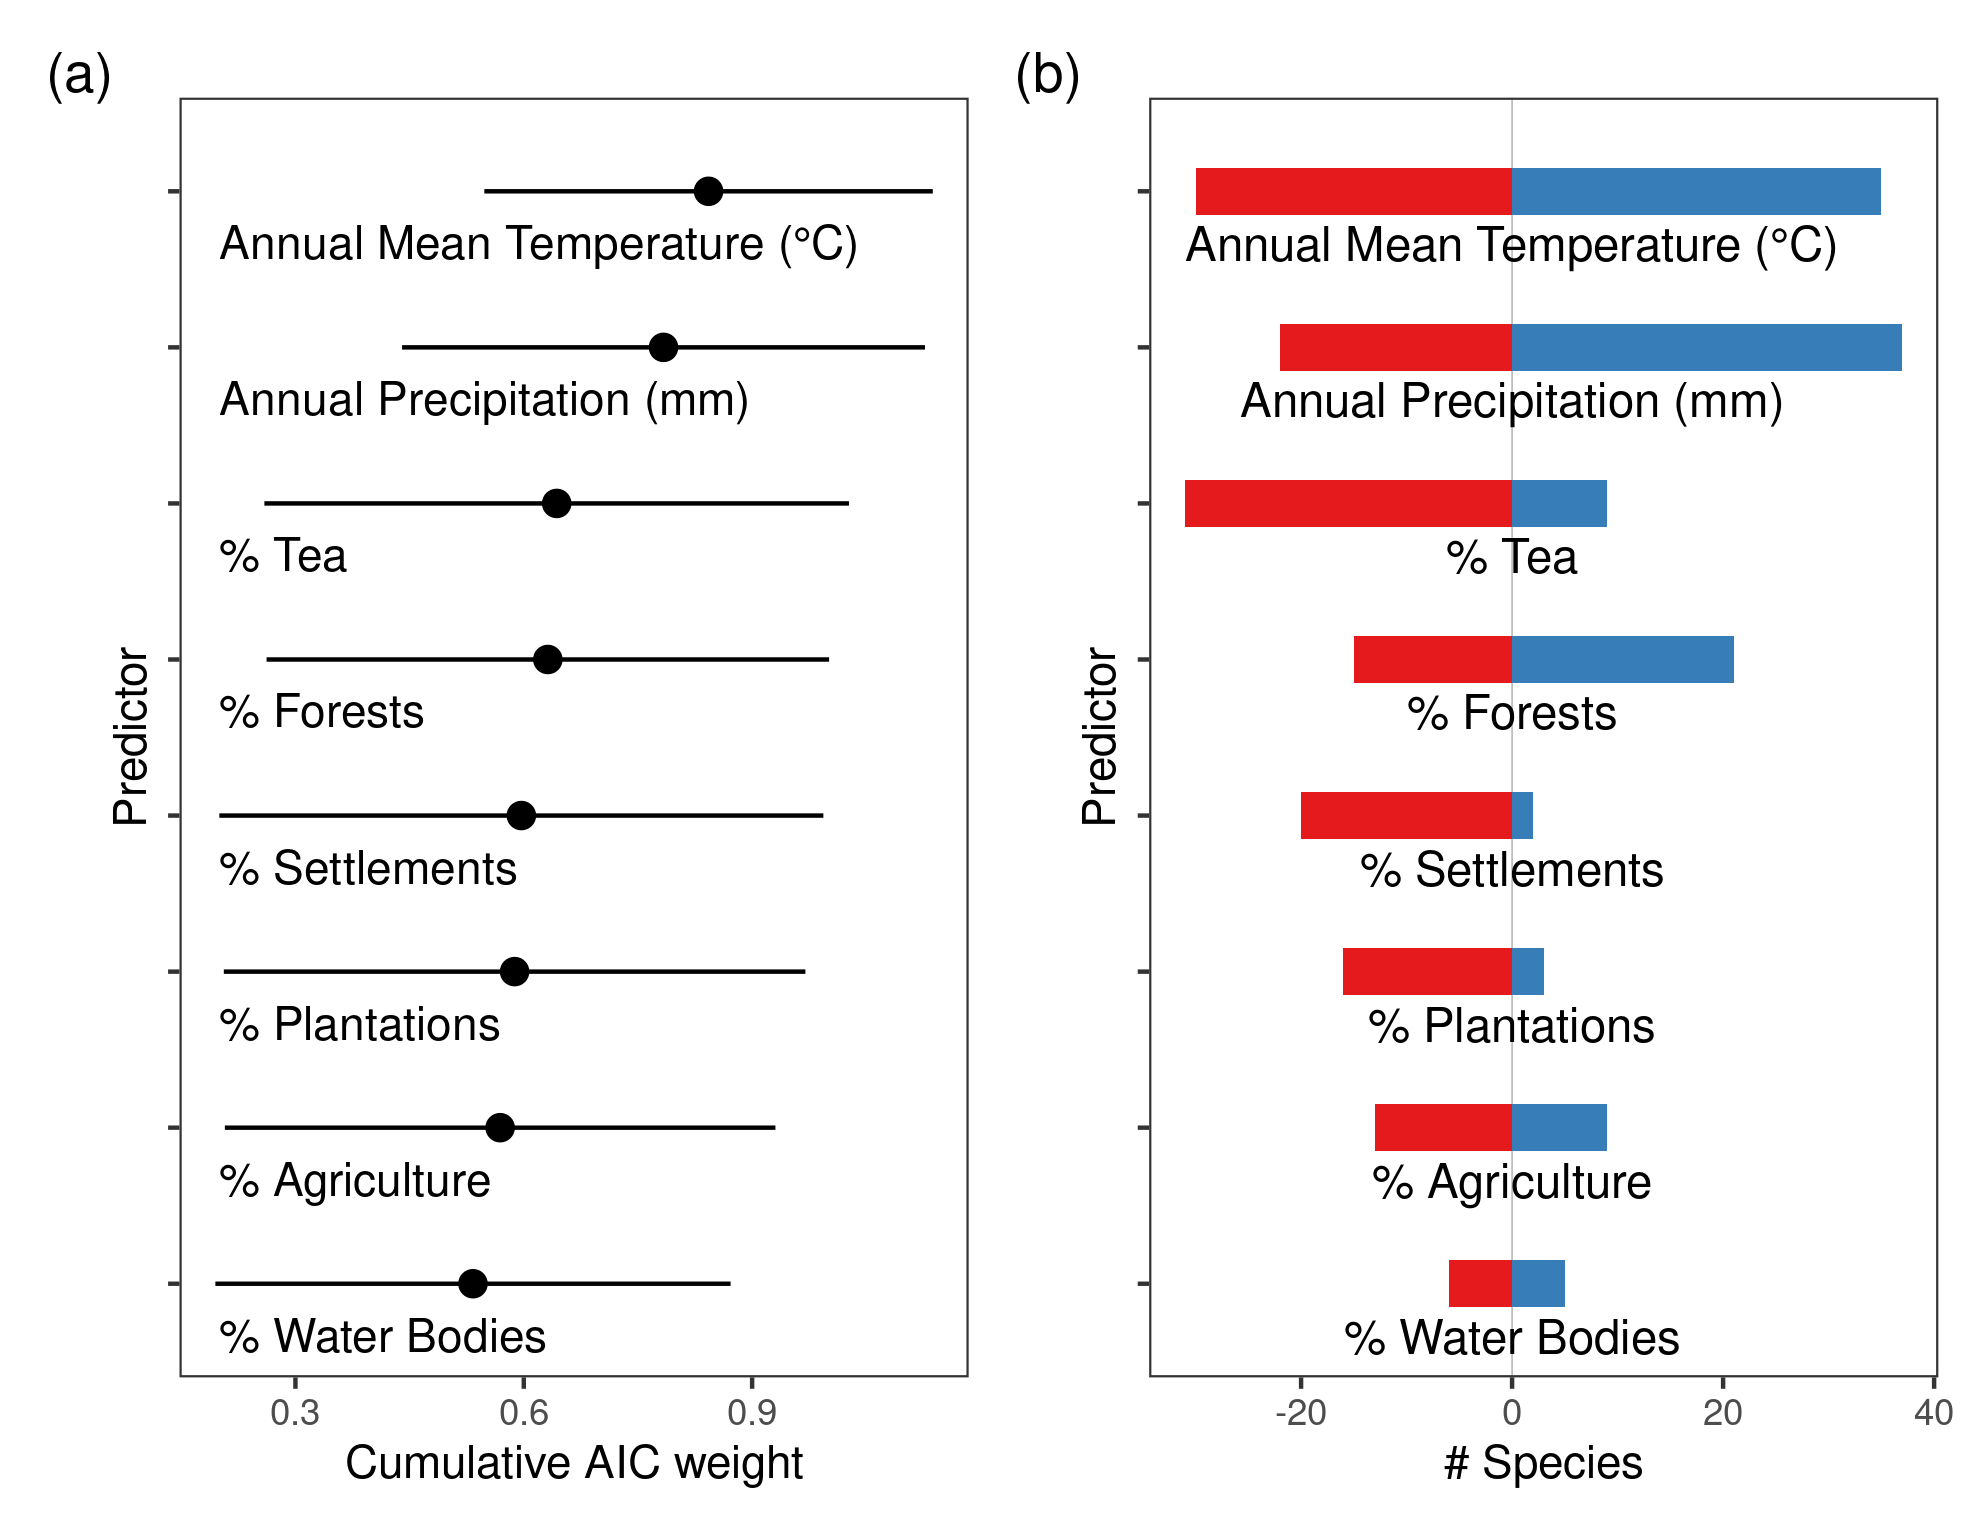
\includegraphics{figs/fig_04_aic_weight_effect.png}
\caption{(a) Cumulative AIC weights suggest that climatic predictors have higher relative importance when compared to landscape predictors. (b) The direction of association between species-specific probability of occupancy and climatic and landscape is shown here. While climatic predictors were both positively and negatively associated with the probability of occupancy for a number of species, human-associated land cover types were largely negatively associated with species-specific probability of occupancy.}
\end{figure}

\end{document}
